%!TEX program = xelatex

% Name           : hsrm-beamer-minimal.sty
% Author         : Benjamin Weiss (benjamin.weiss@kreatiefton.de)
% Version        : 0.2
% Created on     : 08.05.2013
% Last Edited on : 24.03.2014
% Copyright      : Copyright (c) 2013 by Benjamin Weiss. All rights reserved.
% License        : This file may be distributed and/or modified under the
%                  GNU Public License.
% Description    : HSRM beamer theme minimal example.

\documentclass{beamer}

\usepackage[german]{babel}
\usepackage{amsmath, xspace, multirow, color, rotating, adjustbox}
\usetheme[noflama]{hsrm}
%\nosectionpages

\newcommand*{\ttbar}{\ensuremath{\lowercase{t\bar{t}}}\xspace}
\newcommand*{\mtw}{\ensuremath{\text{m}_{\text{T}}^{W}}\xspace}
\newcommand*{\mww}{\ensuremath{\text{m}_{WW}}\xspace}
\newcommand*{\mhh}{\ensuremath{\text{m}_{hh}}\xspace}
\newcommand*{\pt}{\ensuremath{p_{\text{T}}}\xspace}
\newcommand*{\ptbb}{\ensuremath{p_{\text{T}}^{b\bar{b}}}\xspace}
\newcommand*{\ptww}{\ensuremath{p_{\text{T}}^{WW}}\xspace}
\newcommand*{\mbb}{\ensuremath{\text{m}_{b\bar{b}}}\xspace}
\newcommand*{\dsig}{\ensuremath{|d_{0}/\sigma_{d_{0}}|}\xspace}
\newcommand*{\dphi}{\ensuremath{\Delta\phi (\ell,\nu)}\xspace}
\newcommand*{\drbb}{\ensuremath{\Delta\text{R}_{b\bar{b}}}\xspace}
\newcommand*{\drww}{\ensuremath{\Delta\text{R}_{WW}}\xspace}
\newcommand*{\Wtb}{\ensuremath{W\lowercase{tb}}\xspace}
\newcommand*{\fo}{\ensuremath{F_{\text{0}}}\xspace}
\newcommand*{\fl}{\ensuremath{F_{\text{L}}}\xspace}
\newcommand*{\fr}{\ensuremath{F_{\text{R}}}\xspace}
\newcommand*{\bt}{\ensuremath{b}\xspace}
\newcommand*{\syst}{\mbox{$\;$(syst.)}\xspace}
\newcommand*{\mt}{\ensuremath{m_{t}}\xspace}
\newcommand*{\bbWW}{\ensuremath{\lowercase{b\bar{b}}WW^*}\xspace}
\newcommand{\bbbar}{\ensuremath{b\bar{b}}\xspace}

\newcommand\Wider[2][3em]{%
  \makebox[\linewidth][c]{%
    \begin{minipage}{\dimexpr\textwidth+#1\relax}
      \raggedright#2
    \end{minipage}%
  }%
}


\title{Measurement of W-Helicity\protect\\ Fractions in \ttbar decays and\protect\\ Search for Exotic Dihiggs\protect\\ Production in the \protect \lowercase{$b\bar{b}$}$WW^*$\protect\\ Decay Channel Using\protect\\ the ATLAS Detector}
\subtitle{ }

\author{Benjamin Tannenwald}
%\institute{on behalf of the ATLAS Collaboration}
\date{19 June 2017}


\begin{document}

\maketitle

{ % to delimit a block (we only want to remove the header for this frame)

  \makeatletter % to change template
  \setbeamertemplate{headline}[default]
  \def\beamer@entrycode{\vspace*{-1.075\headheight}}
  \begin{frame} {Where Are We Going?}
    \begin{enumerate}
    \item Theory
      \begin{itemize}
      \item Standard Model
      \item Higgs mechanism
      \item Top quark
      \end{itemize}
    \item Experiment
      \begin{itemize}
      \item LHC
       \item ATLAS (and all its subsystems)
      \end{itemize}
    \item Measuring W-helicity using \ttbar decays
      \begin{itemize}
      \item Selecting + reconstructing \ttbar events
      \item Extracting helicity fractions
      \item Limits on anomalous couplings
      \end{itemize}
    \item A search for dihiggs production in the \bbWW final state
      \begin{itemize}
      \item Selecting + reconstructing possible $hh$ events
      \item Estimating multi-jet QCD
      \item Limits on non-resonant and resonant $hh$ production
      \end{itemize}
    \end{enumerate}
  \end{frame}

  \makeatletter % to change template
  \setbeamertemplate{headline}[default]
  \def\beamer@entrycode{\vspace*{-1.075\headheight}}
  \begin{frame} {The Standard Model (SM)}
    \vspace{5pt}
    \begin{columns}
      \column{.45\textwidth}
      \begin{itemize}\small
      \item Relativistic quantum field theory
      \item Fermionic and bosonic components
      \item Describes three fundamental forces
        \begin{itemize}
        \item Electromagnetic, weak nuclear, and strong nuclear forces 
        \end{itemize}
      \end{itemize}
      \column{.55\textwidth}
      \includegraphics[width=\textwidth]{../figures/standardModel/SMperiodic}
    \end{columns}
    \vspace{-4pt}
    \begin{itemize}\small
    \item Quarks interact via electromagnetic, weak, and strong forces
    \begin{itemize}\footnotesize
    \item Cannot exist as free particles due to QCD confinement
    \end{itemize}
    \item Leptons interact via electromagnetic and weak force (neutrinos only through weak force)
    \item Gauge bosons mediate interactions via the three forces
    \item Particles acquire mass via Higgs mechanism
    \end{itemize}
  \end{frame}

  \makeatletter % to change template
  \setbeamertemplate{headline}[default]
  \def\beamer@entrycode{\vspace*{-1.075\headheight}}
  \begin{frame} {Higgs Mechanism}
  \begin{columns}
    \column{.5\textwidth}
    \begin{itemize}
    \item Proposed in early 1960s
    \item Introduce complex scalar doublet field into SM
      \begin{itemize}
      \vspace{5pt}
      \item$  \phi = 
        \begin{pmatrix}
          \phi^+\\\phi^0
        \end{pmatrix}$
      \end{itemize}
      \vspace{3pt}
      \item Spontaneously breaks electroweak symmetry
      \item Higgs field picks up non-zero vacuum expectation value
      \item Weak bosons ($W^{\pm}, Z$) acquire mass 
      \item Fundamental fermions acquire mass through Yukawa coupling
    \end{itemize}
    \column{.5\textwidth}
    \begin{figure}
      \includegraphics[width=\textwidth]{figures/mexicanHat}
    \end{figure}
    \begin{itemize}
    \item First observed by ATLAS and CMS experiments at CERN in 2012
    \item `Last piece' of the Standard Model
    \end{itemize}
  \end{columns}
  \end{frame}


  \makeatletter % to change template
  \setbeamertemplate{headline}[default]
  \def\beamer@entrycode{\vspace*{-1.075\headheight}}
  \begin{frame} {Higgs Production}
    \vspace{-8pt}
    \begin{columns}
      \column{.5\textwidth}
      \begin{center}\underline{Single Higgs Production}\end{center}\vspace{-10pt}
      \begin{itemize}\footnotesize
      \item Four production modes at hadron collider like LHC
        \item $\sigma_{ggF} = 48.58$ pb
        \item $\sigma_{VBF} = 3.78$ pb
        \item $\sigma_{VH} = 2.25$ pb
        \item $\sigma_{\ttbar H} = 0.51$ pb
      \end{itemize}
      \column{.5\textwidth}
      \vspace{25pt}
      \includegraphics[width=\textwidth]{figures/higgs_prod_mech_pdg}
    \end{columns}
    \vspace{-10pt}
    \begin{center}\underline{Double Higgs Production}\end{center}\vspace{-10pt}
    \begin{itemize}\small
    \item Arises in SM due to Higgs self-interaction and box diagram (left, middle)
    \item Exotic resonances can decay to Higgs boson pairs (right)
    \item $\sigma_{hh} = 33.4$ fb
    \end{itemize}
    \vspace{-10pt}
    \begin{columns}
      \column{.67\textwidth}
      \includegraphics[width=1.1\textwidth]{figures/SM-diHiggs-production}\vspace{-5pt}
      \column{.33\textwidth}
      \includegraphics[width=\textwidth]{../figures/standardModel/BSM-dihiggs-prod_W}
    \end{columns}
    \vspace{-10pt}
    \tiny All cross sections quoted for proton-proton collisions at $\sqrt{s}=13$ TeV
  \end{frame}






  \makeatletter % to change template
  \setbeamertemplate{headline}[default]
  \def\beamer@entrycode{\vspace*{-1.075\headheight}}
  \begin{frame} {Higgs Decay}
    \begin{columns}
      \column{.5\textwidth}
      \begin{itemize}
      \item Higgs couples proportional to mass
        \begin{itemize}
        \item $\sim m_V^2$ for vector bosons
        \item $\sim m_f$ for fermions
        \end{itemize}
      \item Mass of the Higgs sets branching fractions of potential decays
        \begin{itemize}
        \item For $m_h=125$ GeV, $h\rightarrow WW^*$ is second largest branching fraction
        \end{itemize}
      \end{itemize}
      \column{.5\textwidth}
      \includegraphics[width=\textwidth]{../figures/standardModel/higgsXS_BR_125}
    \end{columns}
\Wider{
  \begin{itemize}
  \item In Higgs boson pair production, highest branching fraction is $hh\to \bbbar\bbbar$, but second highest branching fraction is $hh \to \bbWW$
  \begin{itemize}
  \item One Higgs decays via $h\to\bbbar$, other decays via $h\to WW^*$
  \end{itemize}

  \item \bbWW final state interesting to study, especially if \ttbar background is well understood (same final state objects)
  \end{itemize}
  }  
  \end{frame}

  \makeatletter % to change template
  \setbeamertemplate{headline}[default]
  \def\beamer@entrycode{\vspace*{-1.075\headheight}}
  \begin{frame} {Top Quark}
    \begin{itemize}\small
    \item Discovered at Fermilab in 1995
    \item \mt = 173.34$\pm$0.76 GeV (heaviest particle in SM), $\tau_t\sim10^{-25}$ seconds
    \item Large LHC top pair production cross section at LHC ($\sigma_{\ttbar} = 252$ pb @ 8 TeV) means there are lots of tops to study
      \begin{itemize}\footnotesize
      \item Precise measurements of top quark and its properties test predictions of SM at edge of our understanding
      \end{itemize}
    \item Top quark pairs also leading background for $t\bar{t}H$ and $WH$ analyses and BSM searches
    \item Top quarks decay near universally via $t\rightarrow Wb$, classify top decays by $W$ decay (to leptons or quarks)
    \end{itemize}
    \vspace{-3pt}
    \begin{columns}
      \column{.6\textwidth}
      \includegraphics[width=\textwidth]{../figures/standardModel/tt_xsec_vs_s_13TeV}
      \column{.4\textwidth}
      \includegraphics[width=\textwidth]{../figures/standardModel/ttbarDecayChannels_noDilep}
    \end{columns}
  \end{frame}

  \makeatletter % to change template
  \setbeamertemplate{headline}[default]
  \def\beamer@entrycode{\vspace*{-1.075\headheight}}
  \begin{frame}{LHC}
    \vspace{15pt}
    \begin{columns}
      \column{.6\textwidth}
      \includegraphics[width=\textwidth]{figures/LHC_map-s}
      \column{.4\textwidth}
      \includegraphics[width=\textwidth]{../figures/atlasDetector/LHCchain}
    \end{columns}
    \begin{itemize}\small
      \item The Large Hadron Collider (LHC) is a superconducting particle accelerator lying on the Franco-Swiss border that collides particles (proton-proton, proton-lead, and lead-lead) at four interaction points
      \item Main ring has circumference of 27 km, uses 1232 dipole magnets cooled to 1.9 K, and can accelerate protons to a maximum design momentum of 14 TeV/c
      \item ATLAS detector is one of four main detectors positioned at the interaction points where the beams collide
    \end{itemize}
  \end{frame}

  \makeatletter % to change template
  \setbeamertemplate{headline}[default]
  \def\beamer@entrycode{\vspace*{-1.075\headheight}}
  \begin{frame}{ATLAS: A T\lowercase{oroidal} L\lowercase{HC} A\lowercase{pparatu}S }
    \vspace{10pt}
    \begin{columns}
      \column{.65\textwidth}
      \includegraphics[width=\textwidth]{../figures/atlasDetector/atlas-large-annotated}
      \column{.35\textwidth}
      \includegraphics[width=\textwidth]{figures/ATLASslice}
    \end{columns}
    %\vspace{-10pt}
    \begin{itemize}\small
    \item ATLAS is composed of multiple subsystems sensitive to a wide variety of phenomena over large range of particle energies
    \item Provides near complete (hermetic) solid angle coverage to completely surround interaction point and detect particles produced in collisions
    \item With $\sim100$ million readout channels and weighing about 7000 tons, ATLAS is the largest particle detector ever built
    \end{itemize}
  \end{frame}

  \makeatletter % to change template
  \setbeamertemplate{headline}[default]
  \def\beamer@entrycode{\vspace*{-1.075\headheight}}
  \begin{frame}{ATLAS: Magnet System}
    \vspace{10pt}
    \begin{columns}
      \column{.65\textwidth}
      \includegraphics[width=1.1\textwidth]{../figures/atlasDetector/exp-magnets}
      \column{.35\textwidth}
      \begin{itemize}\small
        \item Bends the paths of charged particles produced in collisions
        \item Allows for precise determinations of charged particle momenta
        \end{itemize}  
    \end{columns}
    \vspace{-5pt}
    \begin{itemize}\small
    \item ATLAS uses hybrid magnet system composed of one central superconducting solenoid and three exterior toroids (one central and two endcaps)    
    \item Central solenoid cooled to 4.5 K and produces magnetic field of 2.0 T
    \item Each toroid composed of eight radially symmetric superconducting coils cooled to 4.6 K
    \item Barrel (central) toroid produces magnetic field of 0.5 T, endcap toroids produce magnetic field of 1.0 T
    \end{itemize}  
  \end{frame}
  
  \makeatletter % to change template
  \setbeamertemplate{headline}[default]
  \def\beamer@entrycode{\vspace*{-1.075\headheight}}
  \begin{frame}{ATLAS: Inner Detector}
    \begin{columns}
      \column{.6\textwidth}
      \includegraphics[width=1.1\textwidth]{../figures/atlasDetector/atlas-innerDetector}
      \column{.4\textwidth}
      \begin{itemize}\small
      \item Designed to measure passage of charged particles produced in collisions while minimally affecting their trajectories and energies
      \item Composed of central and endcap silicon pixel detectors, silicon strip detectors, and transition radiation (TRT) detectors
      \end{itemize}  
    \end{columns}
    \begin{columns}
      \column{.6\textwidth}  
      \begin{itemize}\small
      \item Silicon pixels and strips arranged in three concentric rows in central region
        \begin{itemize}\footnotesize
        \item Fourth inner layer added in 2013-2014 to improve tracking performance
        \end{itemize}
        \vspace{-4pt}
      \item TRT composed of gas-filled straw drift tubes designed to differentiate between electrons and pions
      \end{itemize}  
      \column{.4\textwidth}  
      \includegraphics[width=\textwidth]{../figures/atlasDetector/PionRejVsEtaWithMC}
    \end{columns}
  \end{frame}

  \makeatletter % to change template
  \setbeamertemplate{headline}[default]
  \def\beamer@entrycode{\vspace*{-1.075\headheight}}
  \begin{frame}{ATLAS: Calorimetry}
    \vspace{5pt}
    \begin{columns}
      \column{.35\textwidth}
      \begin{itemize}\small
      \item ATLAS has electromagnetic and hadronic calorimetry systems
      \item Together provide precise energy measurements of electrons, photons, and hadrons (jets) produced in collisions
      \end{itemize}  
      \column{.65\textwidth}
      \includegraphics[width=1.1\textwidth]{../figures/atlasDetector/atlas-calo-high}
    \end{columns}
    \vspace{-5pt}
    \begin{itemize}\small
      \item Both calorimeters use alternating layers of absorbing material designed to initiate showers from passing particles and layers of active material responsible for measuring the energies of passing particles 
    \item Electromagnetic calorimeter made of alternating layers of a liquid argon sampling medium and lead absorber plates
    \item Hadronic calorimeter has a central alternating scintillating plastic/steel tile component and two liquid argon/copper endcaps
    \end{itemize}  
  \end{frame}
  
  \makeatletter % to change template
  \setbeamertemplate{headline}[default]
  \def\beamer@entrycode{\vspace*{-1.075\headheight}}
  \begin{frame}{ATLAS: Muon Systems}
    \begin{columns}
      \column{.6\textwidth}
      \includegraphics[width=\textwidth]{../figures/atlasDetector/atlas-muonSpectrometer}
      \column{.4\textwidth}
      \begin{itemize}\footnotesize
      \item Last system encountered by particles produced at interaction point
      \item Charged particles reaching the muon spectrometer are nearly always muons
      \item Particles from secondary interactions in detector rejected by requiring tracks from muon spectrometer to match tracks from the inner detector
      \end{itemize}  
    \end{columns}
    %\vspace{-5pt}
    \begin{columns}
      \column{.65\textwidth}
      \begin{itemize}\small
      \item Monitored drift tubes and cathode strip chambers measure energy of passing charged particles
      \item Resistive plate and thin gap chambers provide spatial information and inputs used in muon-based triggering

      \end{itemize}  
      \column{.35\textwidth}
      \includegraphics[width=.95\textwidth]{../figures/atlasDetector/fakesMuidPt}
   \end{columns}
  \end{frame}

  \makeatletter % to change template
  \setbeamertemplate{headline}[default]
  \def\beamer@entrycode{\vspace*{-1.075\headheight}}
  \begin{frame}{ATLAS: Missing Energy Reconstruction}
    \vspace{10pt}
    \begin{columns}
      \column{.5\textwidth}
      \includegraphics[width=\textwidth]{../figures/objectDefinitions/metResolution8TeV_Zmumu}
      \column{.5\textwidth}
      \includegraphics[width=\textwidth]{../figures/objectDefinitions/metResolution13TeV_Zmumu}
    \end{columns}
    \begin{itemize}\small
    \item No way to directly detect high momentum neutrinos (or possible new very weakly interacting particles) produced in some collisions
    \item Instead of measuring the energy/momentum/tracks of these particles, the `missing' transverse energy (MET) in an event is calculated by balancing the total transverse energy measured by the other components (calorimeters, muon systems) 
    \item Resolution of the missing energy calculation measured to be on order of few tens of GeV or less (for most MET algorithms) in events with up to $\sim$1 TeV of energy deposited in the ATLAS detector
    \end{itemize}

  \end{frame}

  \makeatletter % to change template
  \setbeamertemplate{headline}[default]
  \def\beamer@entrycode{\vspace*{-1.075\headheight}}
  \begin{frame}{ATLAS: Triggering and Data Accquisition}
    \begin{itemize}\small
    \item Rate of $\sim$ 40 million collisions per second produces many more events than can reasonably be recorded
    \item To select and save interesting events, used three-level trigger system during data-taking between 2010-2012 
      \begin{itemize}\footnotesize
      \item Improvements in the trigger algorithms and hardware enabled use of a two-level trigger during data-taking in 2015-2016
      \end{itemize}
    \item First trigger level (L1) is a hardware-based trigger that uses a small subset of the total calorimeter and muon spectrometer information to decide in under 2.5 $\mu$s whether or not to keep an event
    \item L1 decision reduces event rate to $\sim75$ kHz
      % In 2010-2012 data-taking, a secondary L2 trigger re-processes events passing the L1 stage using more complete detector information from the muon spectrometer and inner detector systems.
    \item For events passing L1 trigger (and similar L2 stage in 2010-2012), software based high level trigger (HLT) uses the full amount of data collected by the detector (including track and vertex reconstruction) to select events
    \item HLT computer farm processes events in $\sim$4 seconds and produces an output rate of $\sim$200 Hz
    \item At end of triggering chain, each event is recorded to disc and has a per event size of $\sim$1.3 MB
    \item ATLAS experiment records $\sim$3000 TB of collision data per year
    \end{itemize}
  \end{frame}
  
  \begin{frame}[noframenumbering, plain]
    \vspace{40pt}
    \begin{center}
      \huge
      W-Helicity Measurement @ 8 TeV
    \end{center}
  \end{frame}

  \makeatletter % to change template
  \setbeamertemplate{headline}[default]
  \def\beamer@entrycode{\vspace*{-1.075\headheight}}
  \begin{frame}{W-Helicity Measurement}
    \Wider{
      \vspace{6pt}
      \begin{itemize}
        \footnotesize
      \item Extract fractions of left-handed, right-handed, and longitudinally polarized $W$ bosons in semileptonic $t\bar{t}$ decays
        \begin{itemize}
          \scriptsize
        \item Relative fractions are well predicted by the Standard Model
        \item Deviations could provide solid hint of BSM physics
        \end{itemize}
        \begin{center}\footnotesize$\frac{1}{\sigma}\frac{d\sigma}{d cos\theta^*}=\frac{3}{4}(1-cos^2\theta^*)F_0+\frac{3}{8}(1-cos\theta^*)^2F_L+\frac{3}{8}(1+cos\theta^*)^2F_R$\end{center}
      \end{itemize}
      \vspace{-12pt}
      
      \begin{columns}
        \column{.05\textwidth}
        \column{.5\textwidth}
        \vspace{-5pt}
        \begin{center}\includegraphics[width=.9\textwidth]{figures/costhetaFrame}\end{center}
        
        \column{.5\textwidth}
        \includegraphics[width=.9\textwidth]{figures/SMdistro}
      \end{columns}
      \vspace{-5pt}
      \begin{itemize}
        \footnotesize
      \item Aim to:
        \begin{enumerate}
          \scriptsize
        \item Produce world's best measurements of F$_{0}$, F$_{L}$, and  F$_{R}$
        \item For first time, use direct information from hadronic $W$ decay
        \end{enumerate}
      \end{itemize}
    }
  \end{frame}
  
  \makeatletter % to change template
  \setbeamertemplate{headline}[default]
  \def\beamer@entrycode{\vspace*{-1.075\headheight}}
  \begin{frame}{Previous Measurements}
 \Wider{
      \begin{table}
        \fontsize{7}{8}\selectfont
      \begin{tabular}{c|c|c}
        \hline
        & 7 TeV & 8 TeV\\\hline
        %\multirow{3}{*}{ATLAS} & \multicolumn{2}{c}{\multirow{3}{c}{This analysis!}}\\
        \multirow{4}{*}{\textbf{ATLAS}} & \href{http://link.springer.com/article/10.1007\%2FJHEP06\%282012\%29088}{\color{blue}\underline{JHEP 1206 (2012) 088}}, 1.4 fb$^{-1}$ & \multirow{4}{*}{This analysis!}\\
                               & F$_0$=0.67 $\pm$ 0.03 (stat.) $\pm$ 0.06 (syst.)& \\
                               & F$_L$=0.32 $\pm$ 0.02 (stat.) $\pm$ 0.03 (syst.)& \\
                               & F$_R$=0.01 $\pm$ 0.01 (stat.) $\pm$ 0.04 (syst.)& \\
        %\multirow{3}{*}{ATLAS} & F$_0$=$0.XX\pm0.xx\pm0.XX$ & F$_0$=$0.XX\pm0.xx\pm0.XX$ \\
        %& F$_L$=$0.XX\pm0.xx\pm0.XX$ & F$_L$=$0.XX\pm0.xx\pm0.XX$ \\
        %& F$_R$=$0.XX\pm0.xx\pm0.XX$ & F$_R$=$0.XX\pm0.xx\pm0.XX$ \\
        \hline \hline
        \multirow{4}{*}{\textbf{CMS}} & \href{https://cds.cern.ch/record/1581688/files/jhep.10.167.pdf}{\color{blue}\underline{JHEP 10 (2013) 167}}, 5 fb$^{-1}$ & \href{https://arxiv.org/abs/1605.09047}{\color{blue}\underline{Phys. Lett. B 762 (2016) 512}}, 19.8 fb$^{-1}$\\
                             & F$_0$=0.682 $\pm$ 0.030 (stat.) $\pm$ 0.033 (syst.) & F$_0$=0.681 $\pm$ 0.012 (stat.) $\pm$ 0.023 (syst.) \\
                             & F$_L$=0.310 $\pm$ 0.022 (stat.) $\pm$ 0.022 (syst.) & F$_L$=0.323 $\pm$ 0.008 (stat.) $\pm$ 0.014 (syst.) \\
                             & F$_R$=0.008 $\pm$ 0.012 (stat.) $\pm$ 0.014 (syst.) & F$_R$=-0.004 $\pm$ 0.005 (stat.) $\pm$ 0.014 (syst.) \\
        \hline
      \end{tabular}
    \end{table}
    }
    \vspace{-10pt}
    \begin{itemize}
      \small
    \item F$_0\sim2/3$, F$_L\sim1/3$, F$_R\sim0$ (theory prediction)
    \item 7 TeV ATLAS and CMS used both electron and muon angles in semileptonic $t\bar{t}$ decays
    \item 8 TeV CMS analysis performed using electron and muon angles
      \begin{itemize}
      \item Was previously the most precise measurement
      \end{itemize}
    \item Helicity fractions also measured at Tevatron
      \begin{itemize}
        \footnotesize
      \item Hadronic angle measured indirectly using $|\cos\theta^*|$
      \end{itemize}
    \end{itemize}
  \end{frame}

  \makeatletter % to change template
  \setbeamertemplate{headline}[default]
  \def\beamer@entrycode{\vspace*{-1.075\headheight}}
  \begin{frame}{Dataset + Event Selection}
    \begin{itemize}
      \footnotesize
    \item Use 20.2 fb$^{-1}$ of data from 8 TeV proton-proton collisions recorded by the ATLAS detector in 2012
    \item Monte Carlo simulations used for $t\bar{t}$ signal, W+jets, Z+jets, diboson, and single top
    \item Data-driven methods used to estimate QCD contribution and normalize different W+jets flavor fractions
    \end{itemize}
    \begin{columns}
      \column{.5\textwidth}

      \begingroup
      \small
      \setbeamercolor{block title}{bg=hsrmSec3CompDark}
      \setbeamercolor{block body}{bg=hsrmSec3Comp}
      \begin{block}{Object Selection}
        \scriptsize
        \textbf{Lepton}: p$_{T}^{\ell}$ > 25 GeV, $|\eta^{\ell}|$ < 2.5,\\ Isolated\\
        \textbf{Jets}: Anti-$k_{T}$ $\Delta$R=0.4 jets, p$_{T}^{\text{jet}}$ > 25 GeV, $|\eta^{\text{jet}}|$ < 2.5, $|\text{JVF}|$ > 0.5, 70\% $b$-tagging efficiency\\
        \textbf{MET (1 excl. $b$-tag only):} MET$\geq$20 GeV, MET+m$_{T}^{W}\geq 60$ GeV\\
      \end{block}
      \endgroup
      \column{.5\textwidth}
      \begingroup
      \small
      \setbeamercolor{block title}{bg=hsrmSec2CompDark}
      \setbeamercolor{block body}{bg=hsrmSec2Comp}
      \begin{block}{Event Selection}
        \scriptsize
        \textcolor{white}{
          Lepton trigger\\
          At least 1 primary vertex with $\geq 5$ tracks\\
          N$_{\ell}=1$\\
          N$_{jets}\geq 4$\\
          Categorize by N$_{b\text{-tags}} =1$ or $\geq 2$\\
          Leading log likelihood > -48
        }
      \end{block}
      \endgroup
    \end{columns}
    \begin{itemize}
      \small
    \item Cut on leading log likelihood is quality cut on kinematic fitting algorithm used to reconstruct $t\bar{t}$ system
      \begin{itemize}
      \item More information in coming slides
      \end{itemize}
    \end{itemize}        

  \end{frame}

  \makeatletter % to change template
  \setbeamertemplate{headline}[default]
  \def\beamer@entrycode{\vspace*{-1.075\headheight}}
  \begin{frame}{Kinematic Distributions: Electron Channel, $=1\text{ } \lowercase{ b\text{-tag}}$}
    \vspace{5pt}
    \begin{columns}
      \column{.333\textwidth}
      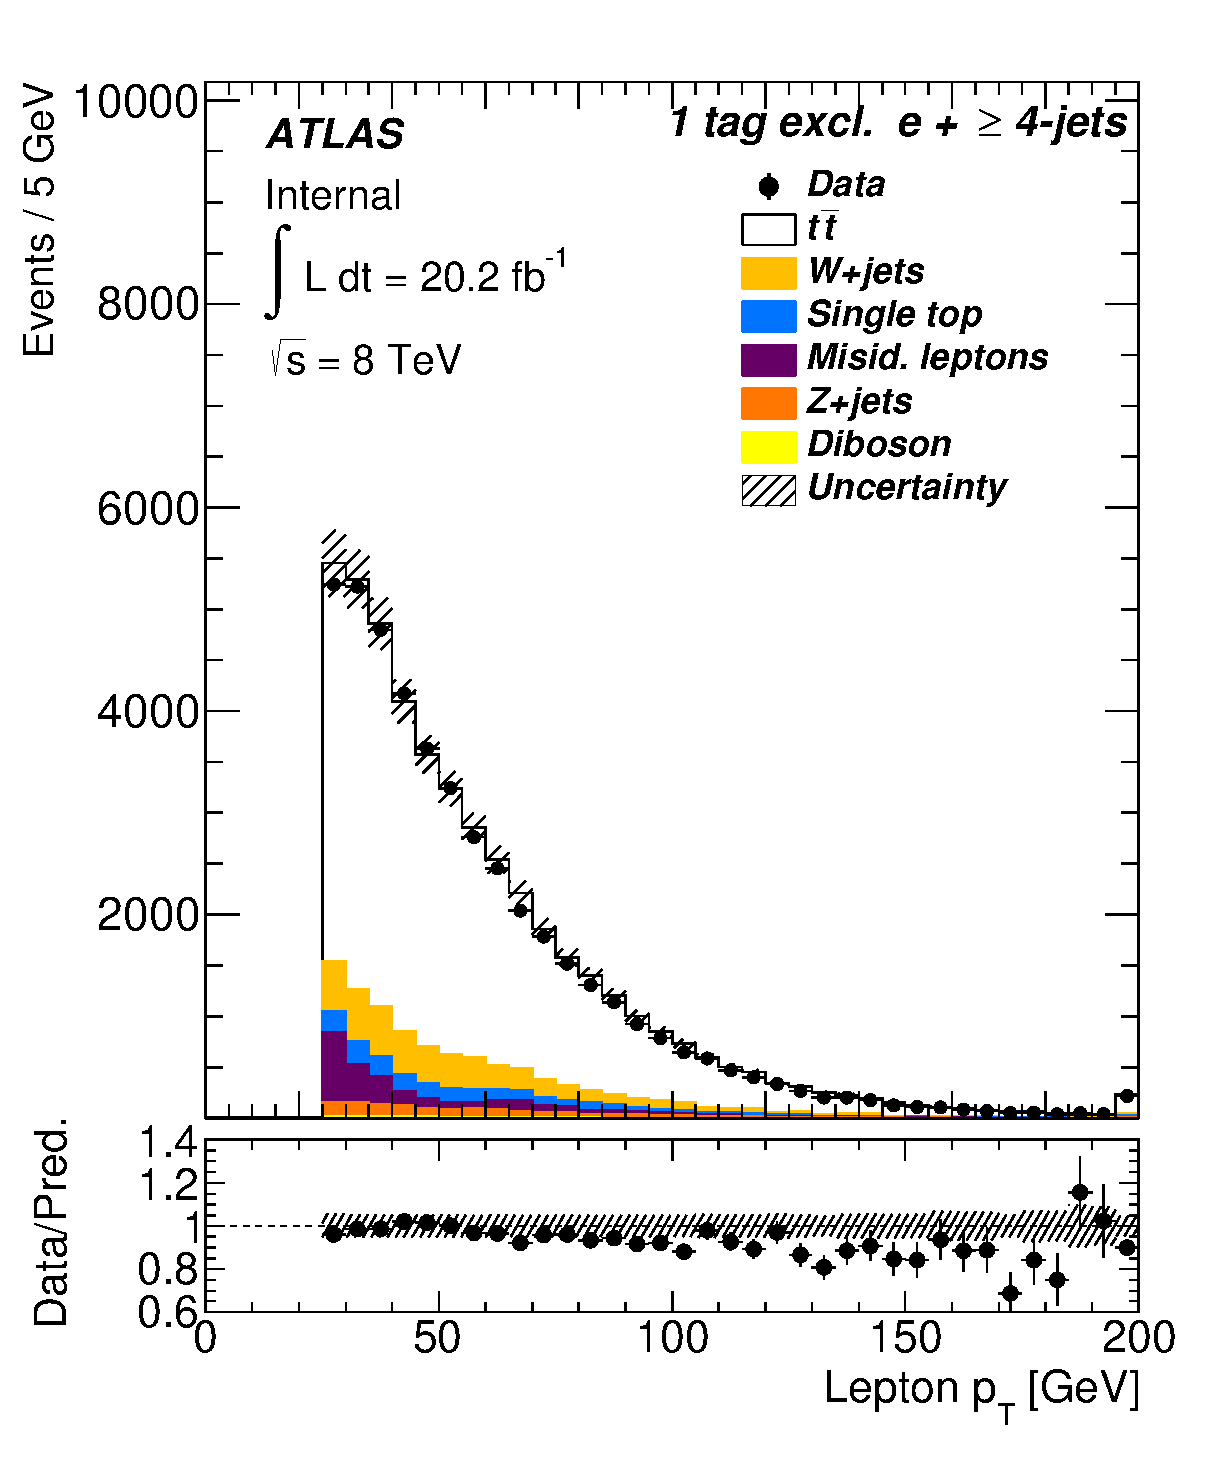
\includegraphics[width=.95\textwidth]{../chapters/whel/figures/control_Plots2/bTag_1excl/LeptonPt_el}\\
      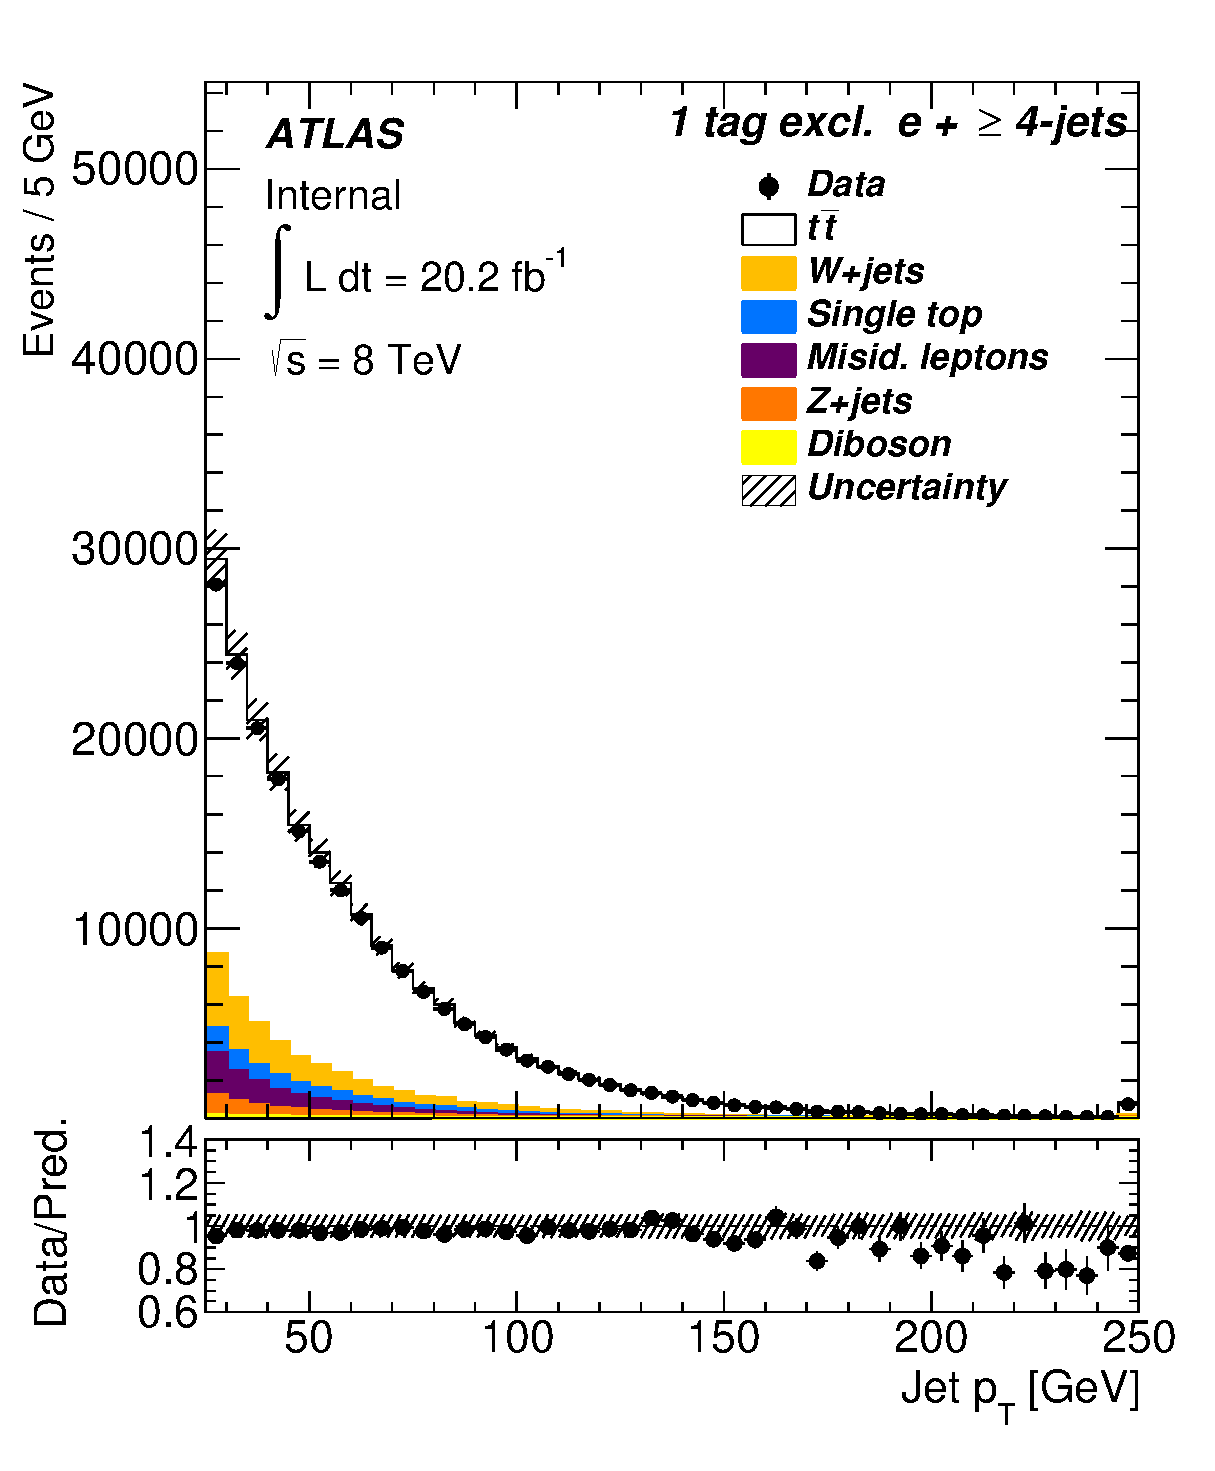
\includegraphics[width=.95\textwidth]{../chapters/whel/figures/control_Plots2/bTag_1excl/JetPt_el}
      \column{.333\textwidth}
      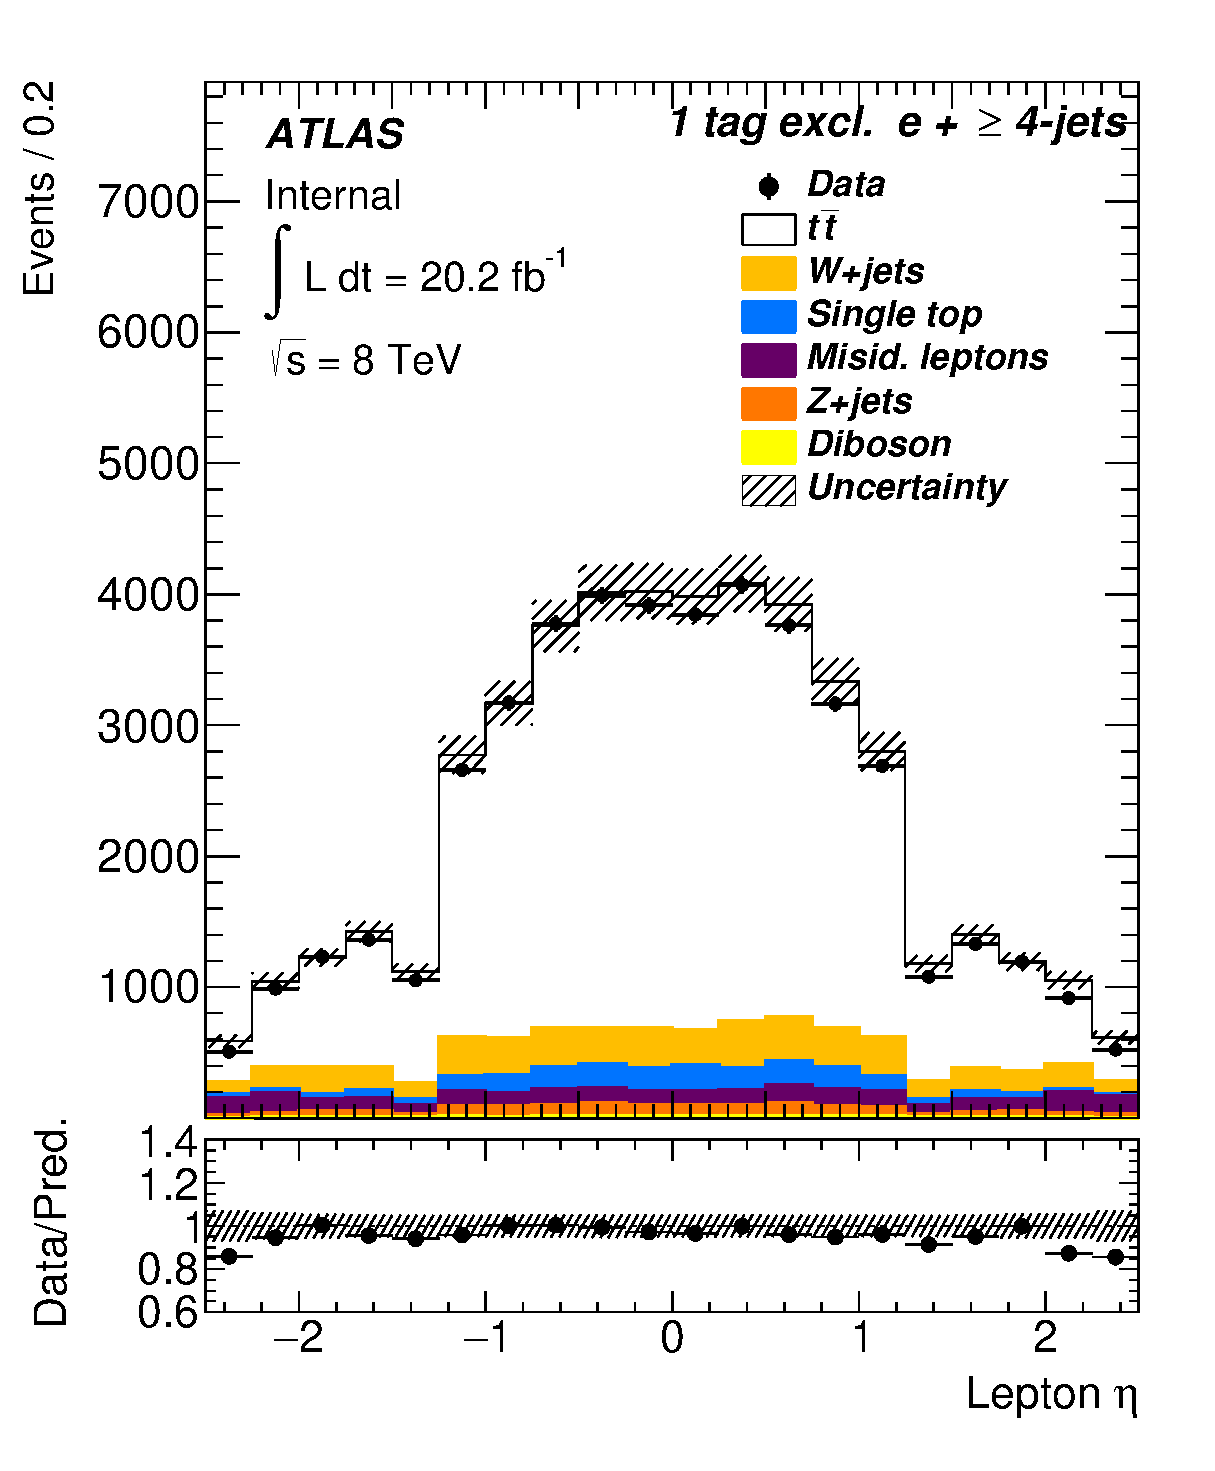
\includegraphics[width=.95\textwidth]{../chapters/whel/figures/control_Plots2/bTag_1excl/LeptonEta_el}\\
      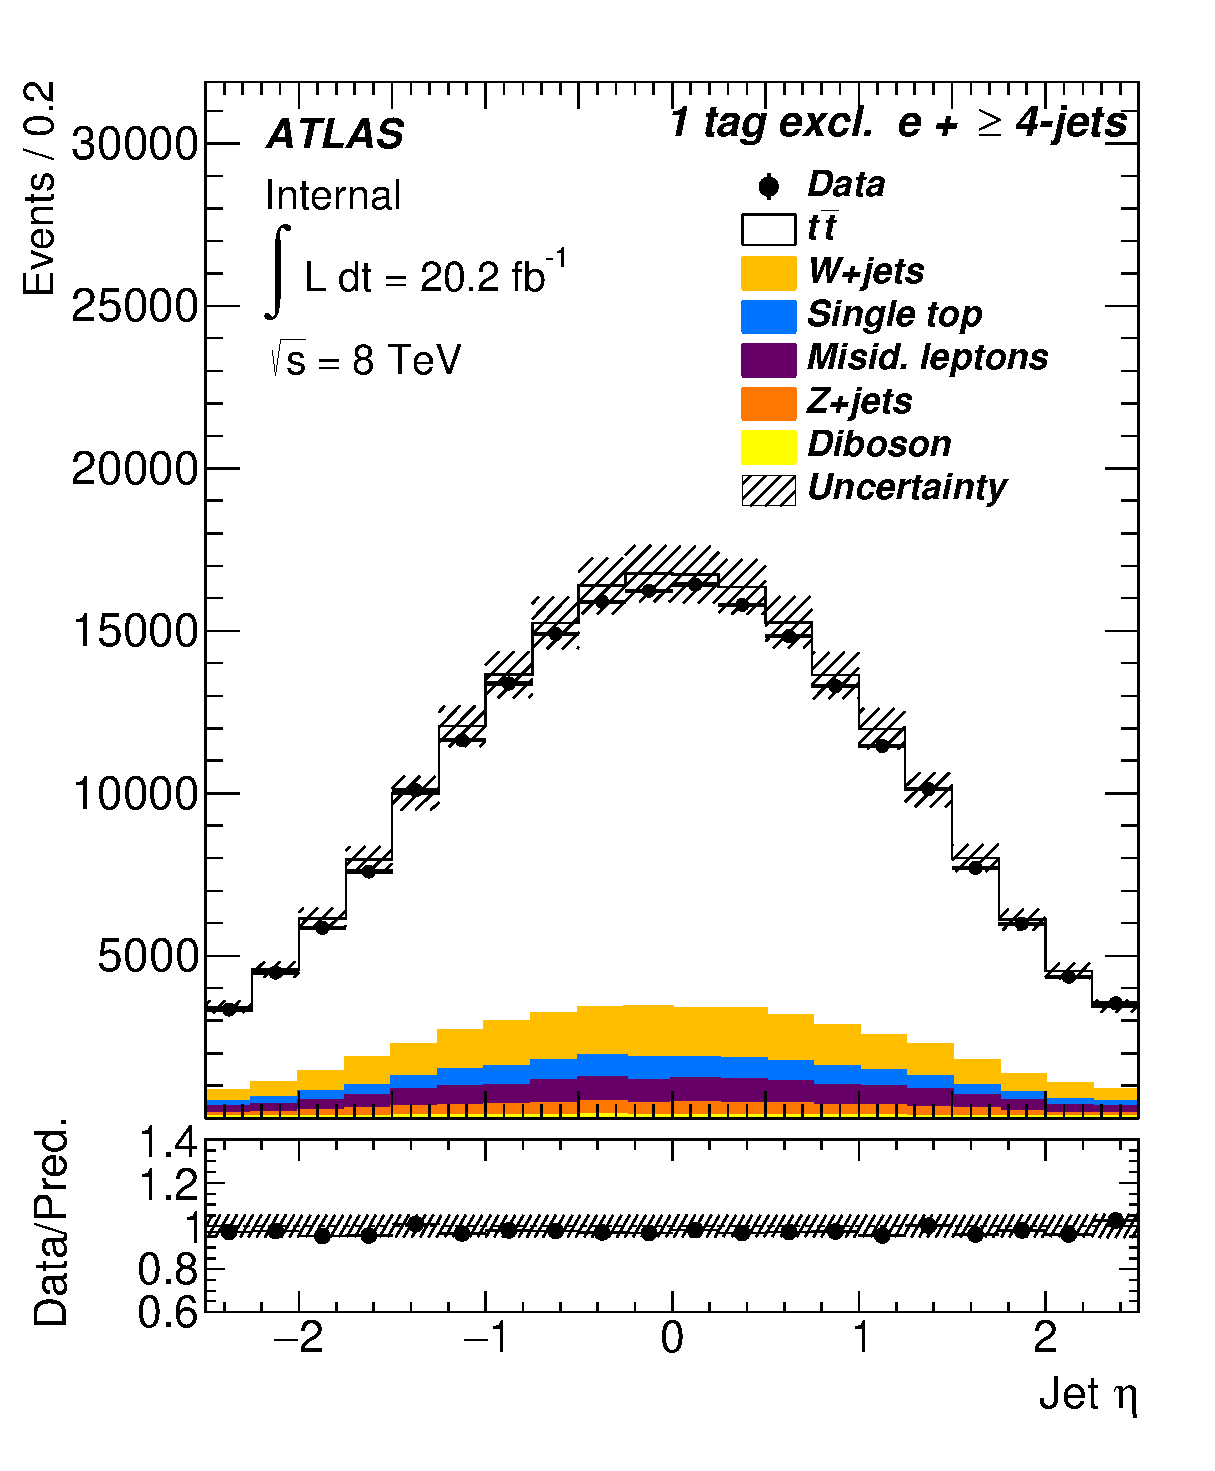
\includegraphics[width=.95\textwidth]{../chapters/whel/figures/control_Plots2/bTag_1excl/JetEta_el}
      \column{.333\textwidth}
      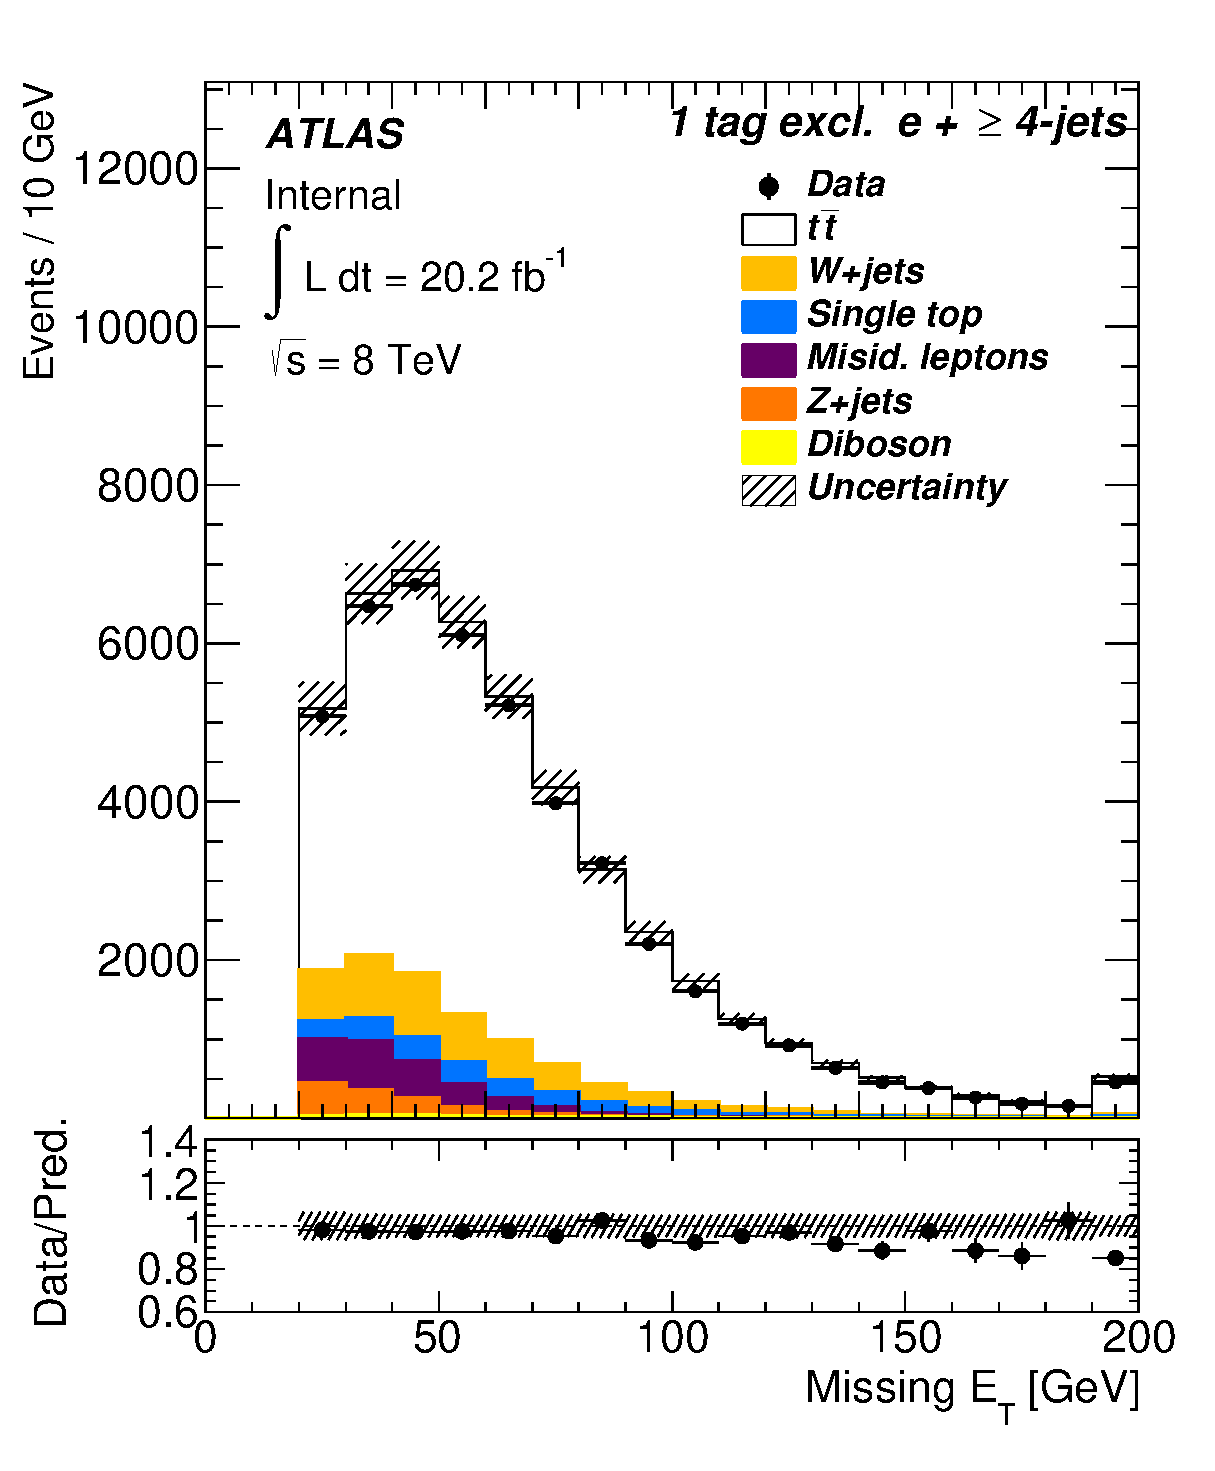
\includegraphics[width=.95\textwidth]{../chapters/whel/figures/control_Plots2/bTag_1excl/MissingEt_el}\\
      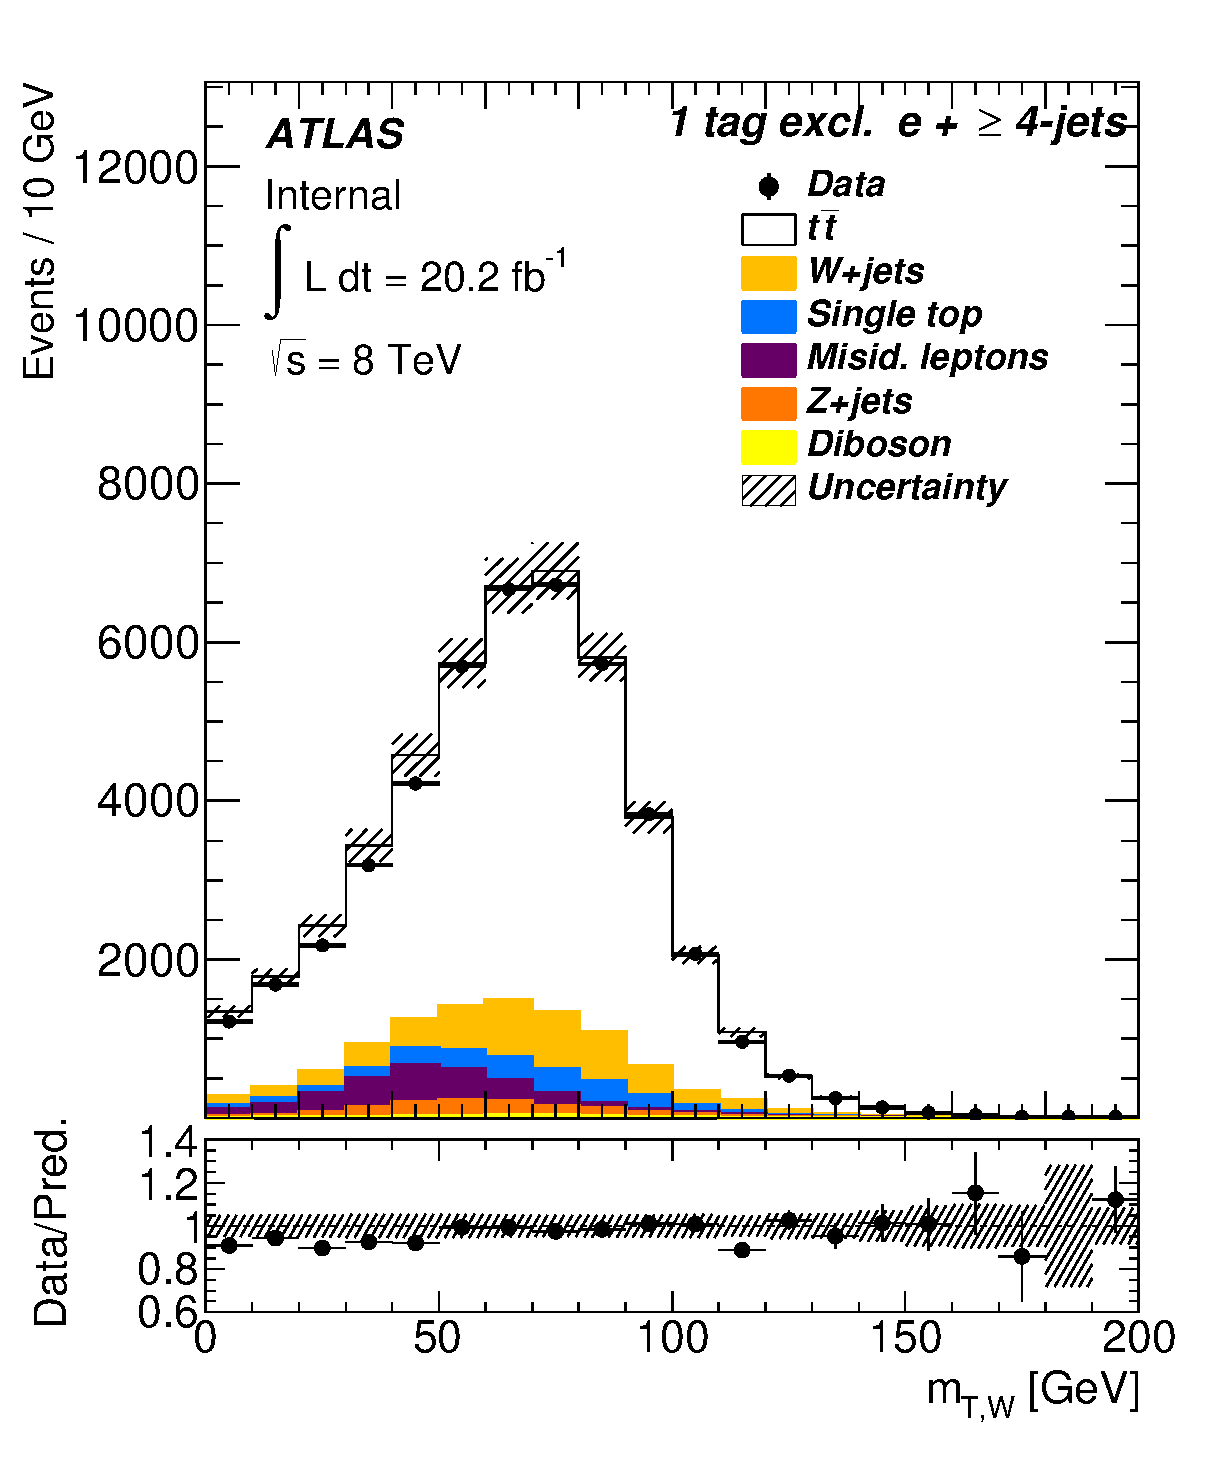
\includegraphics[width=.95\textwidth]{../chapters/whel/figures/control_Plots2/bTag_1excl/TransverseMass_el}
    \end{columns}
  \end{frame}

  \makeatletter % to change template
  \setbeamertemplate{headline}[default]
  \def\beamer@entrycode{\vspace*{-1.075\headheight}}
  \begin{frame}{Kinematic Distributions: Muon Channel, $=1\text{ } \lowercase{ b\text{-tag}}$}
    \vspace{5pt}
    \begin{columns}
      \column{.333\textwidth}
      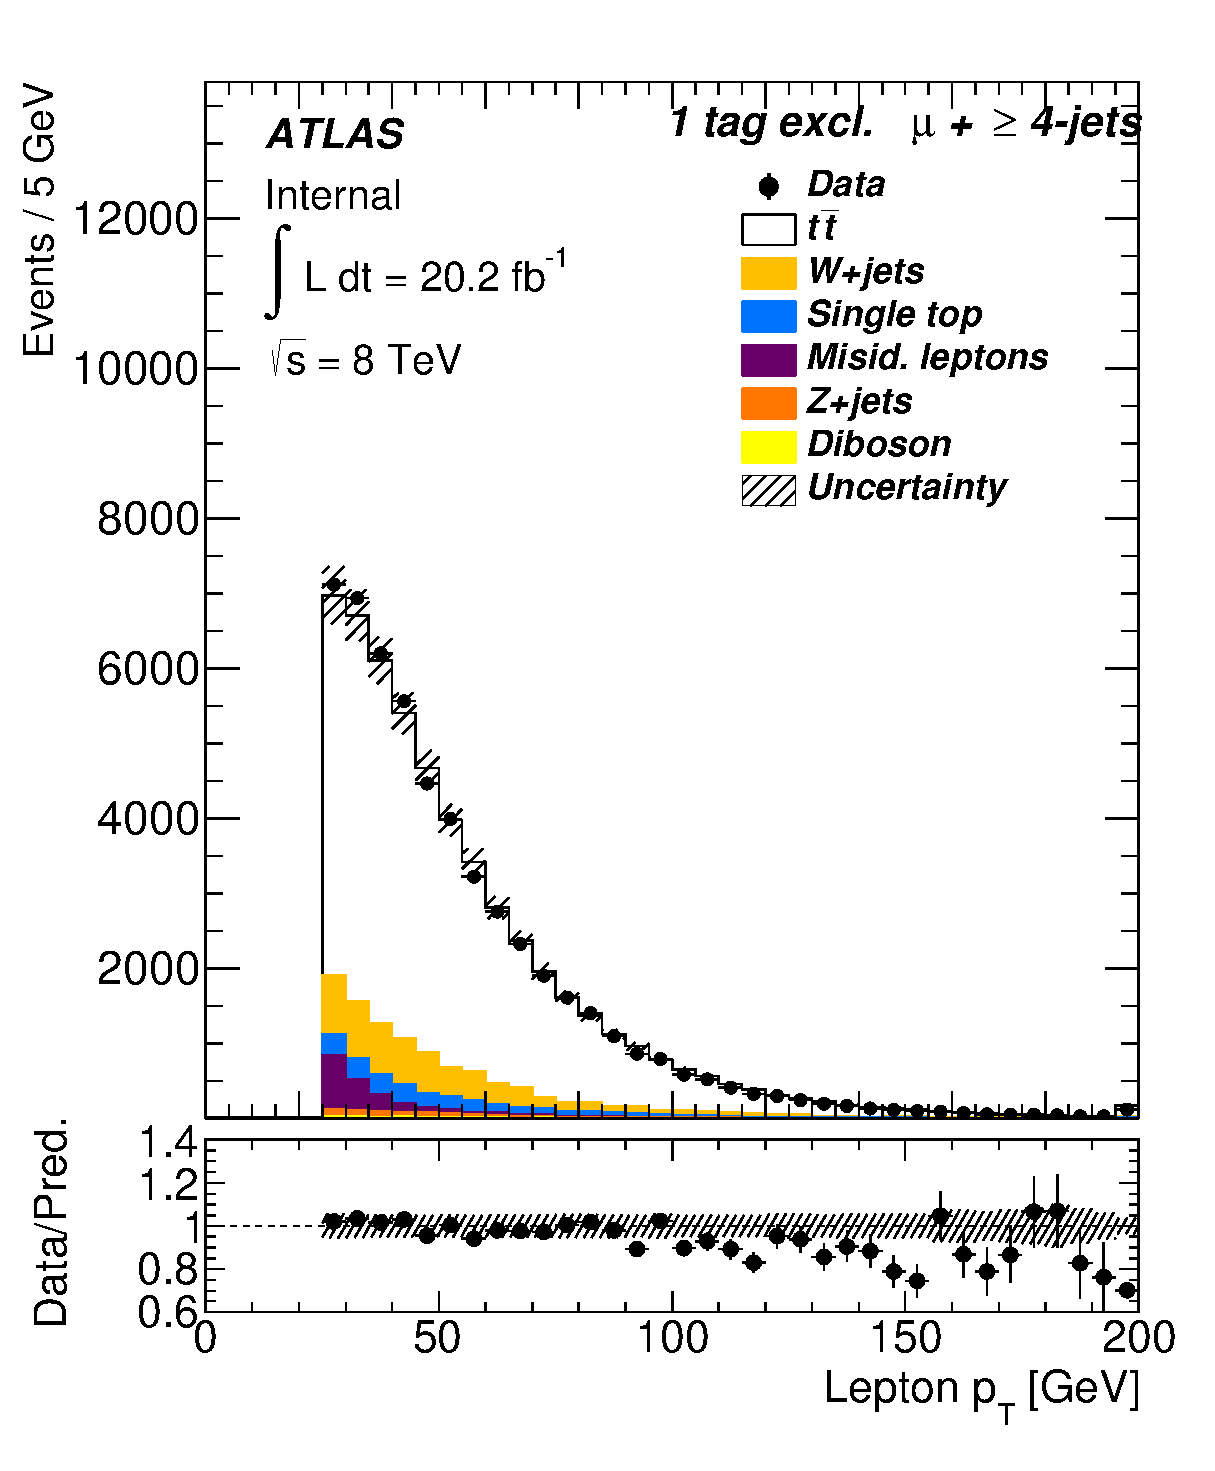
\includegraphics[width=.95\textwidth]{../chapters/whel/figures/control_Plots2/bTag_1excl/LeptonPt_mu}\\
      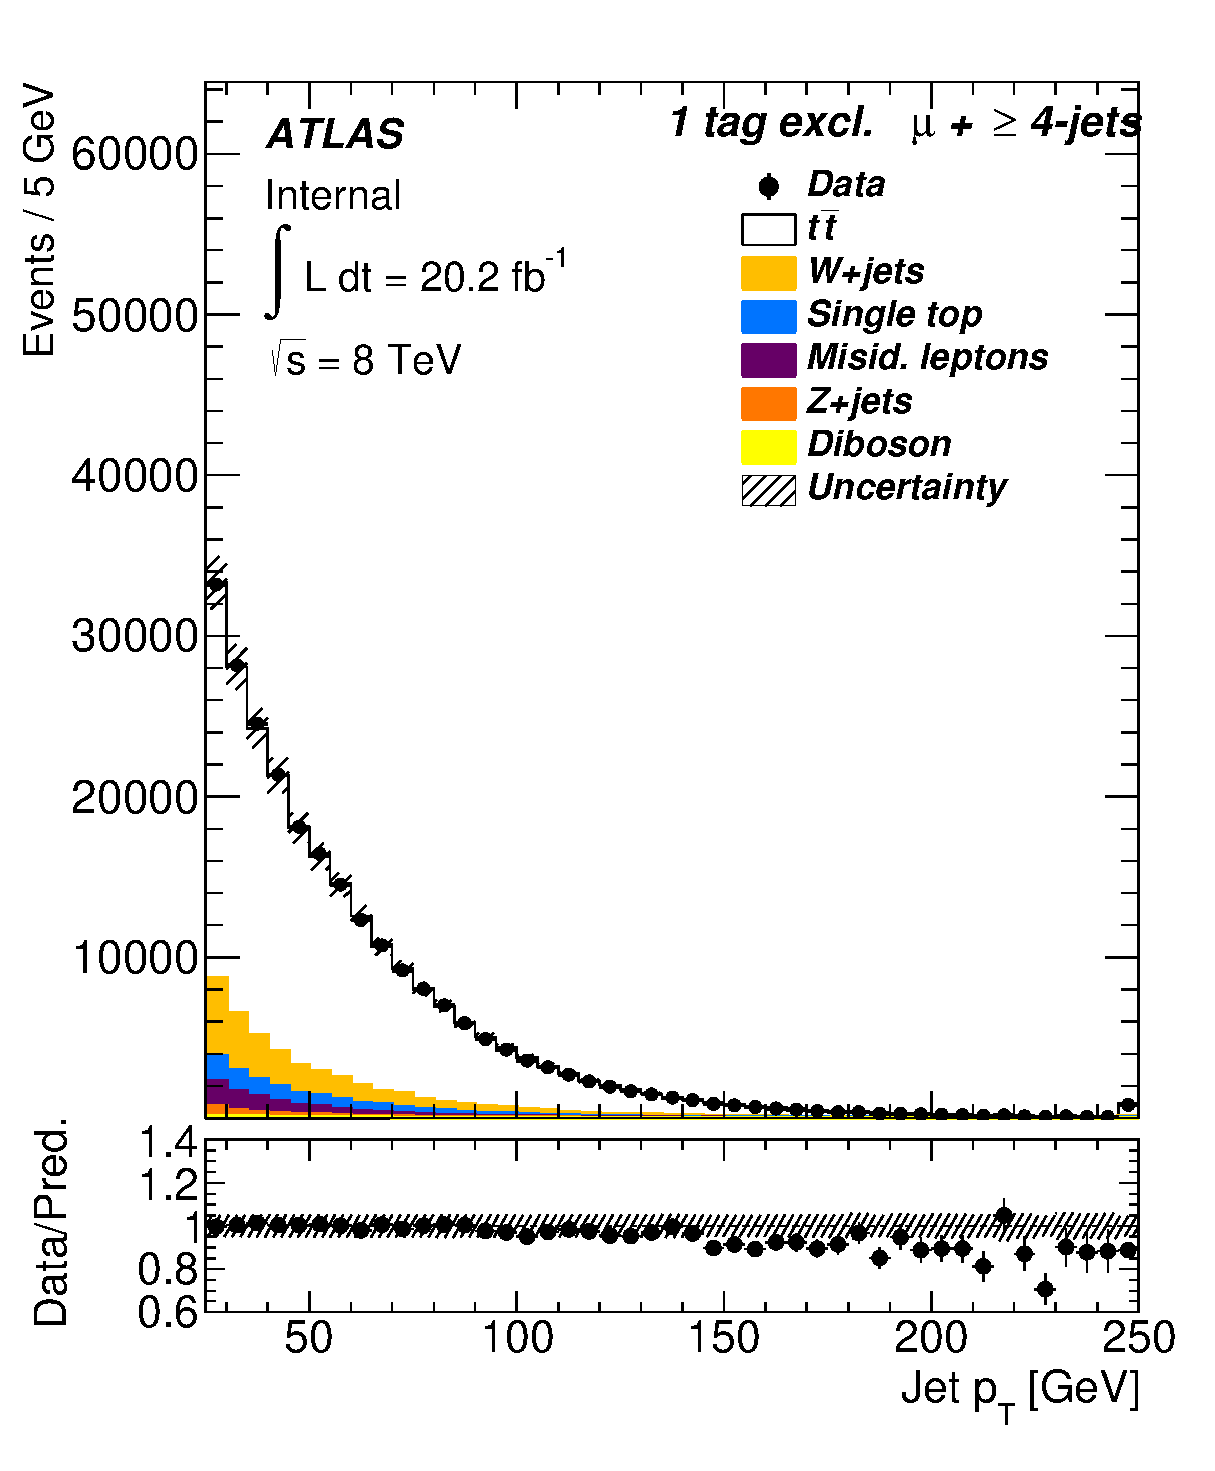
\includegraphics[width=.95\textwidth]{../chapters/whel/figures/control_Plots2/bTag_1excl/JetPt_mu}
      \column{.333\textwidth}
      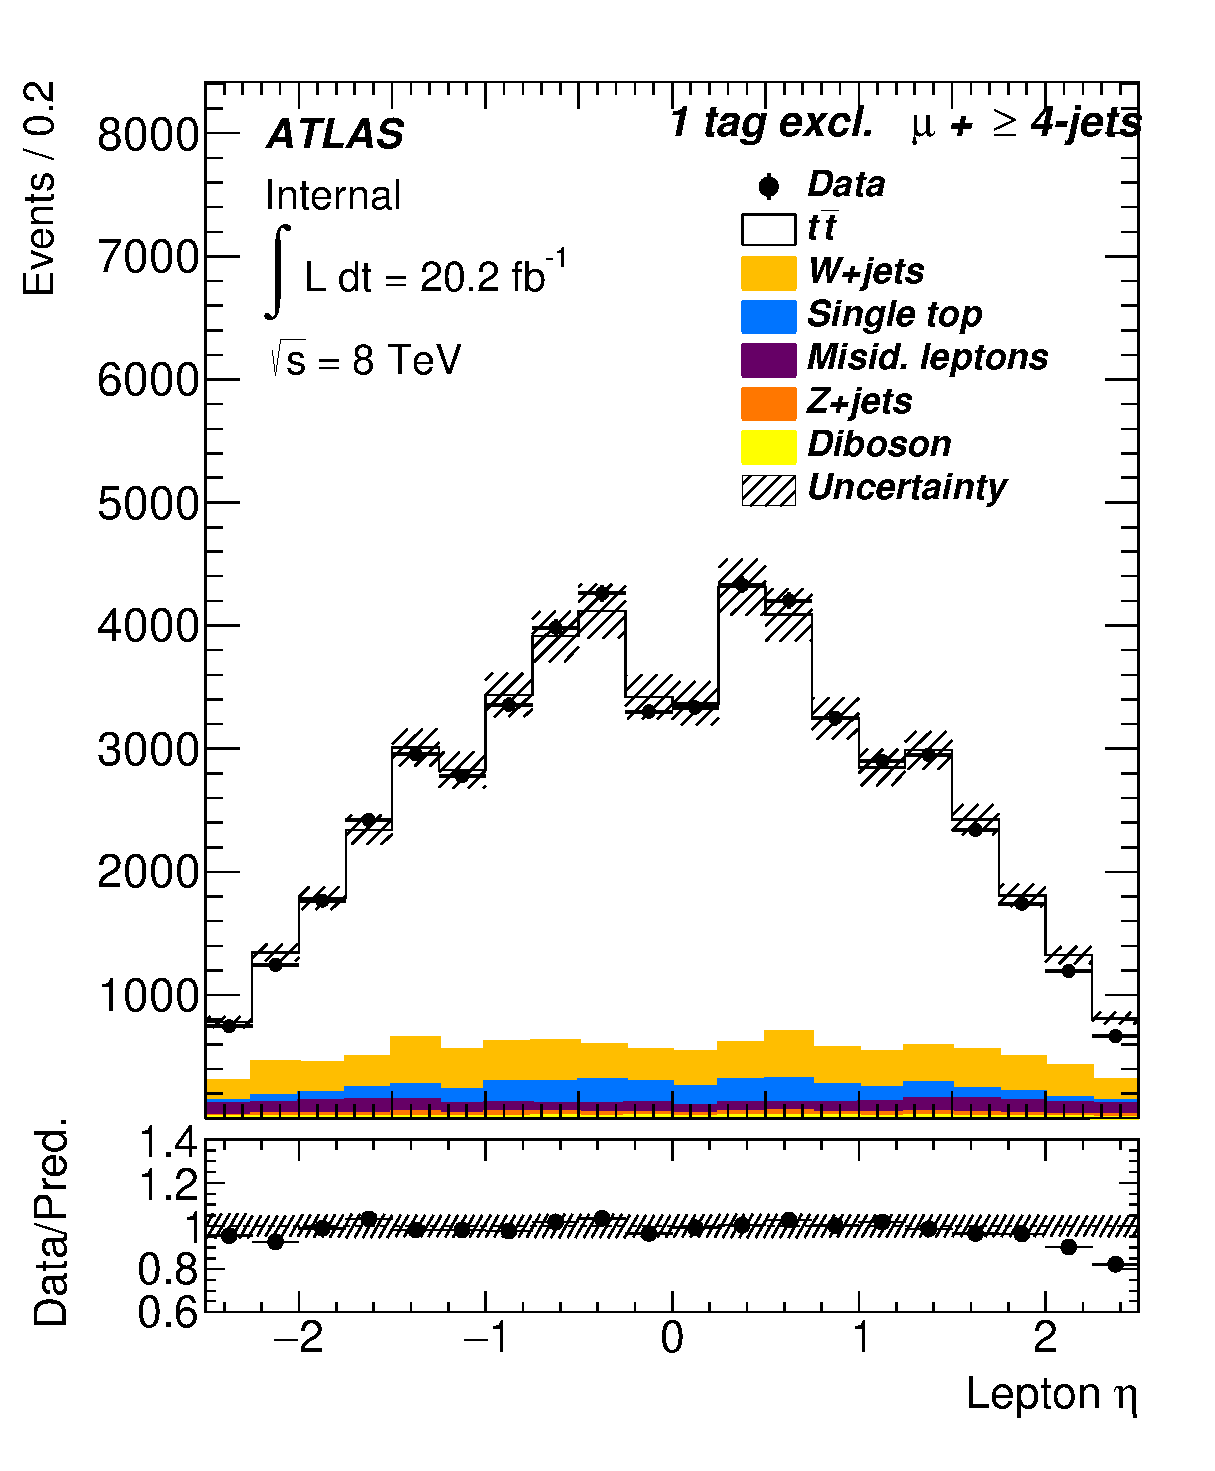
\includegraphics[width=.95\textwidth]{../chapters/whel/figures/control_Plots2/bTag_1excl/LeptonEta_mu}\\
      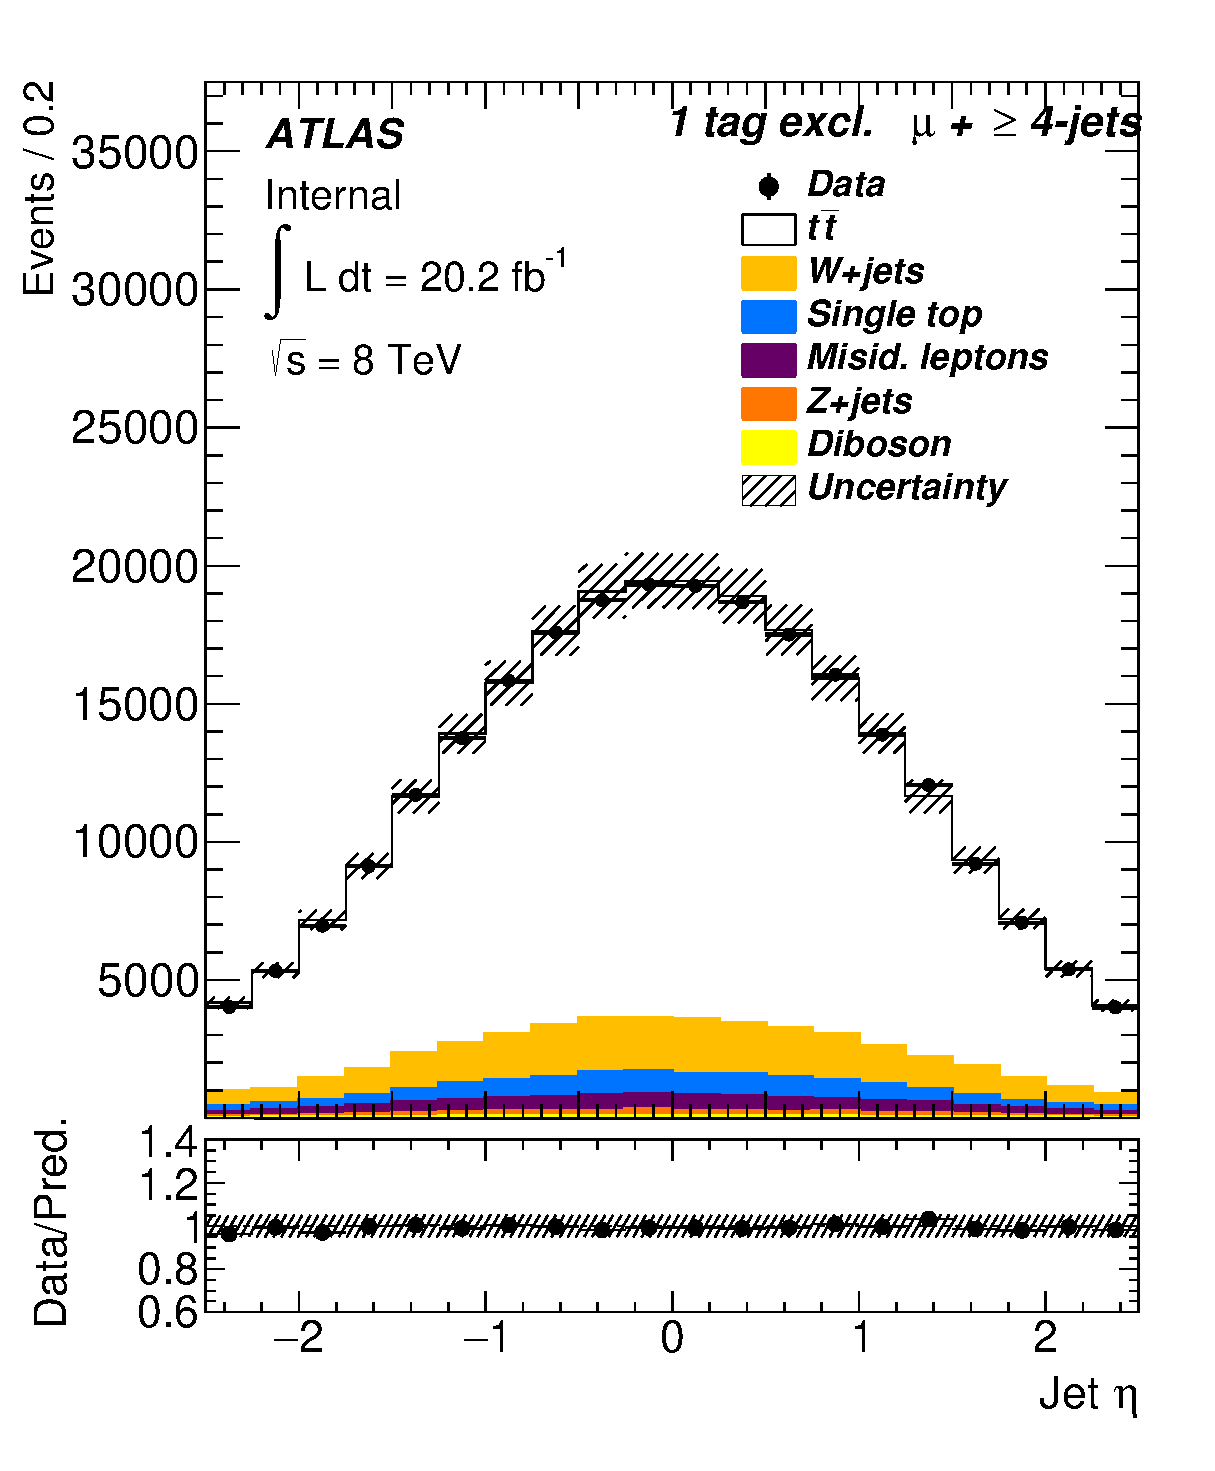
\includegraphics[width=.95\textwidth]{../chapters/whel/figures/control_Plots2/bTag_1excl/JetEta_mu}
      \column{.333\textwidth}
      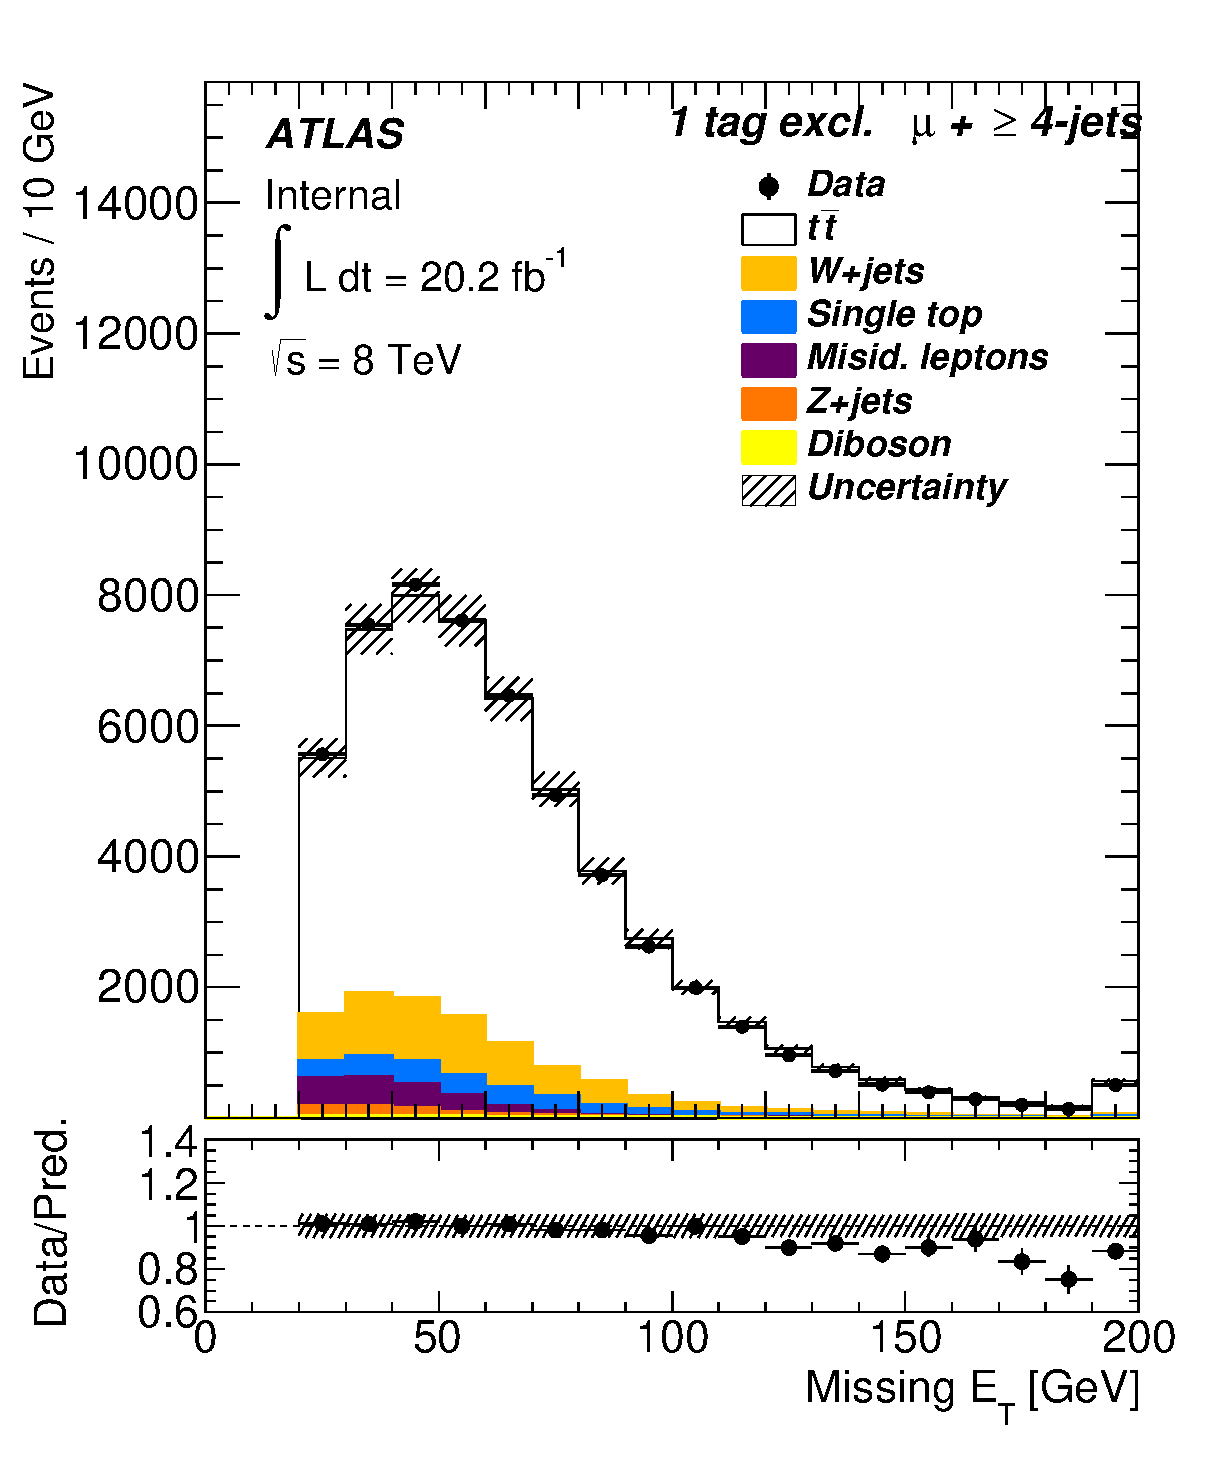
\includegraphics[width=.95\textwidth]{../chapters/whel/figures/control_Plots2/bTag_1excl/MissingEt_mu}\\
      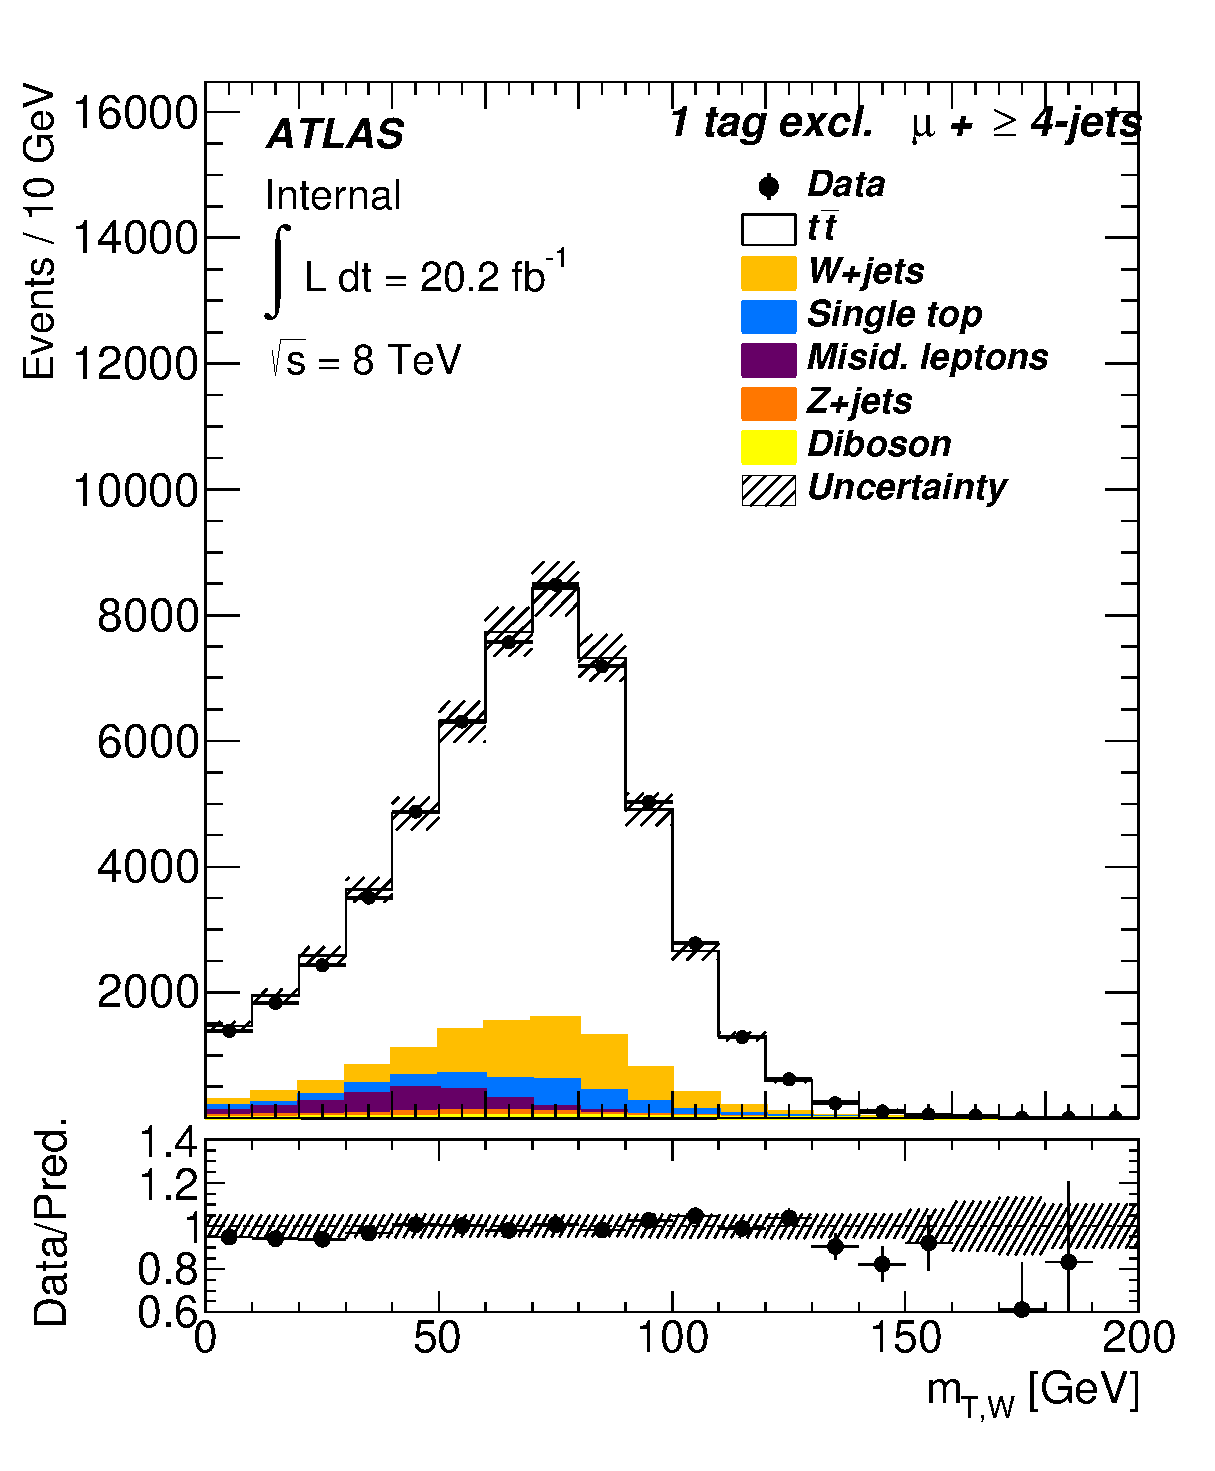
\includegraphics[width=.95\textwidth]{../chapters/whel/figures/control_Plots2/bTag_1excl/TransverseMass_mu}
    \end{columns}
  \end{frame}

  \makeatletter % to change template
  \setbeamertemplate{headline}[default]
  \def\beamer@entrycode{\vspace*{-1.075\headheight}}
  \begin{frame}{Kinematic Distributions: Electron Channel, $\geq2\text{ } \lowercase{ b\text{-tags}}$}
    \vspace{5pt}
    \begin{columns}
      \column{.333\textwidth}
      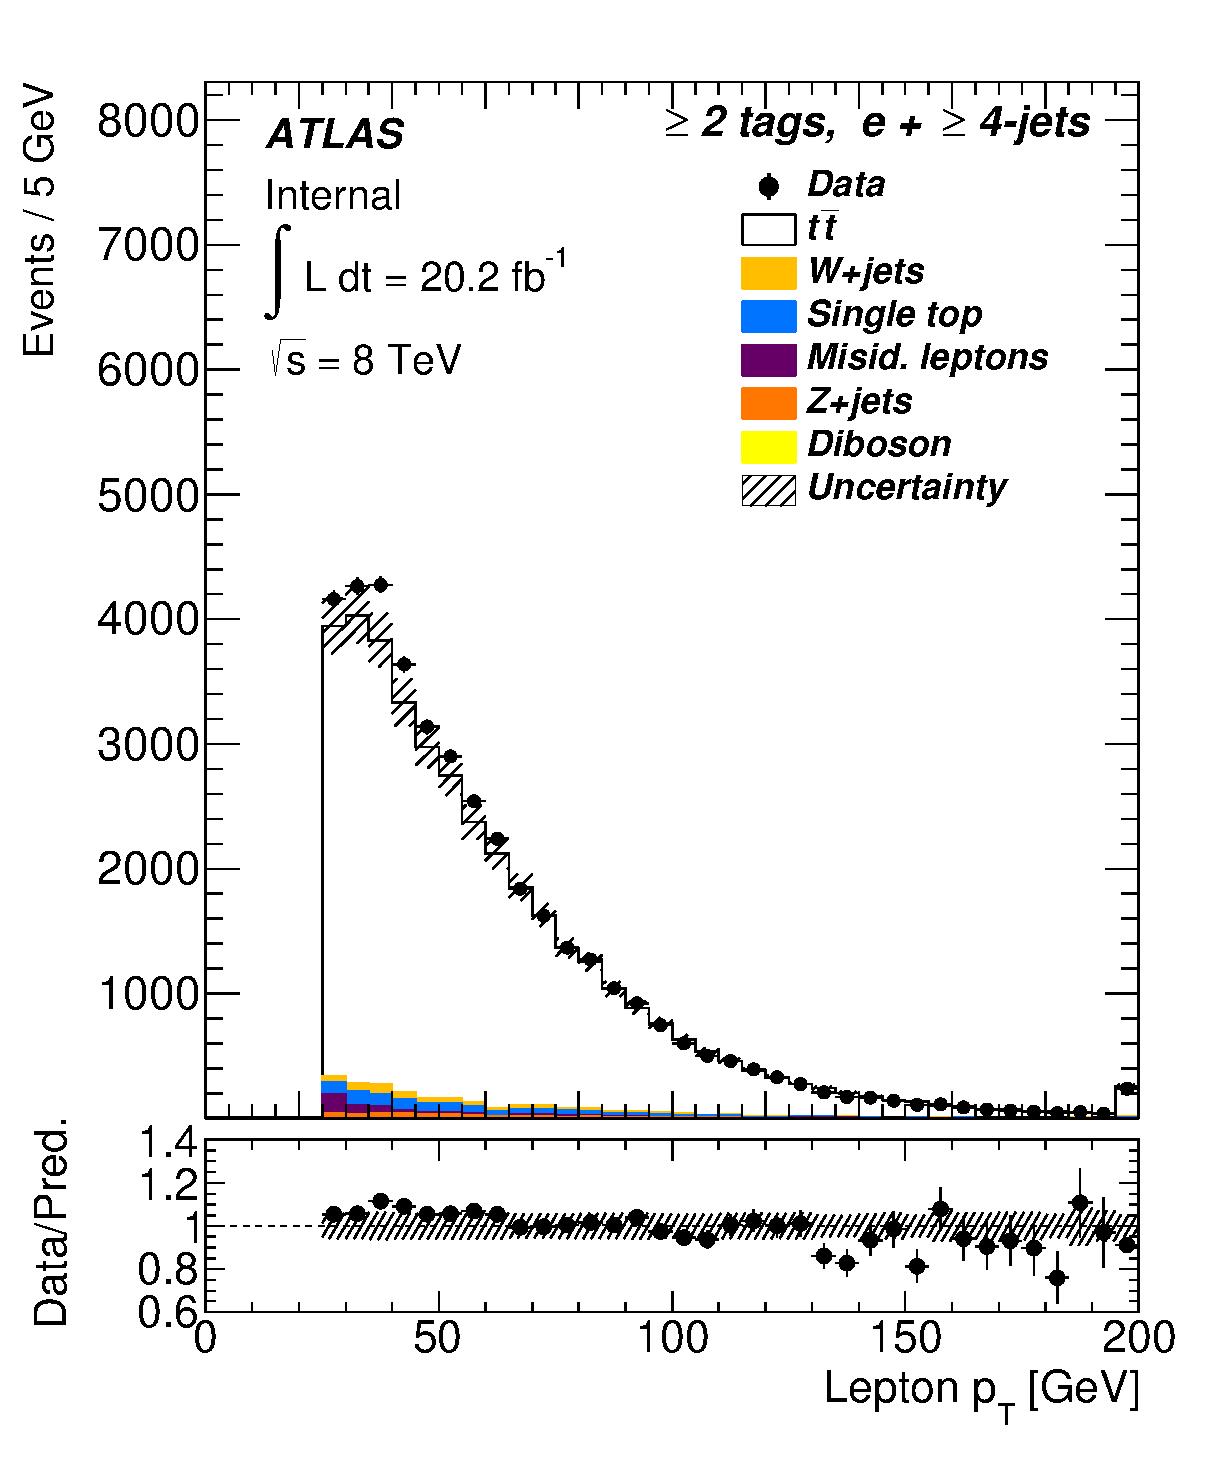
\includegraphics[width=.95\textwidth]{../chapters/whel/figures/control_Plots2/bTag_2incl/LeptonPt_el}\\
      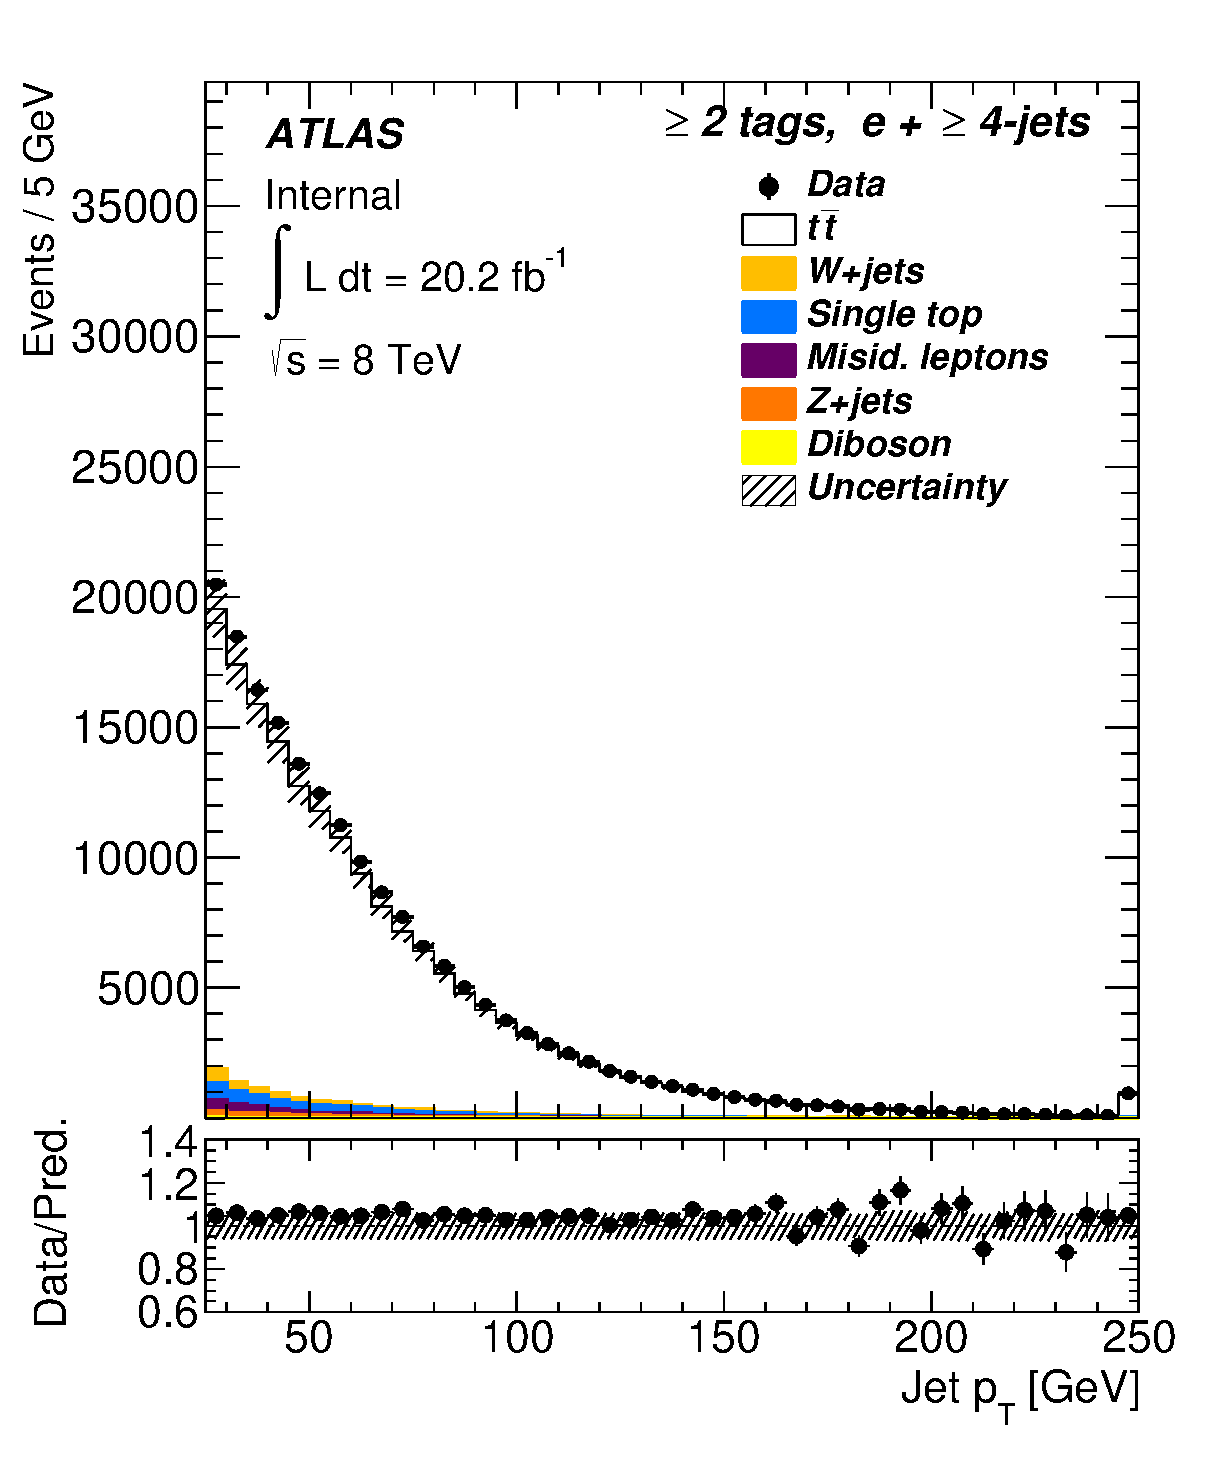
\includegraphics[width=.95\textwidth]{../chapters/whel/figures/control_Plots2/bTag_2incl/JetPt_el}
      \column{.333\textwidth}
      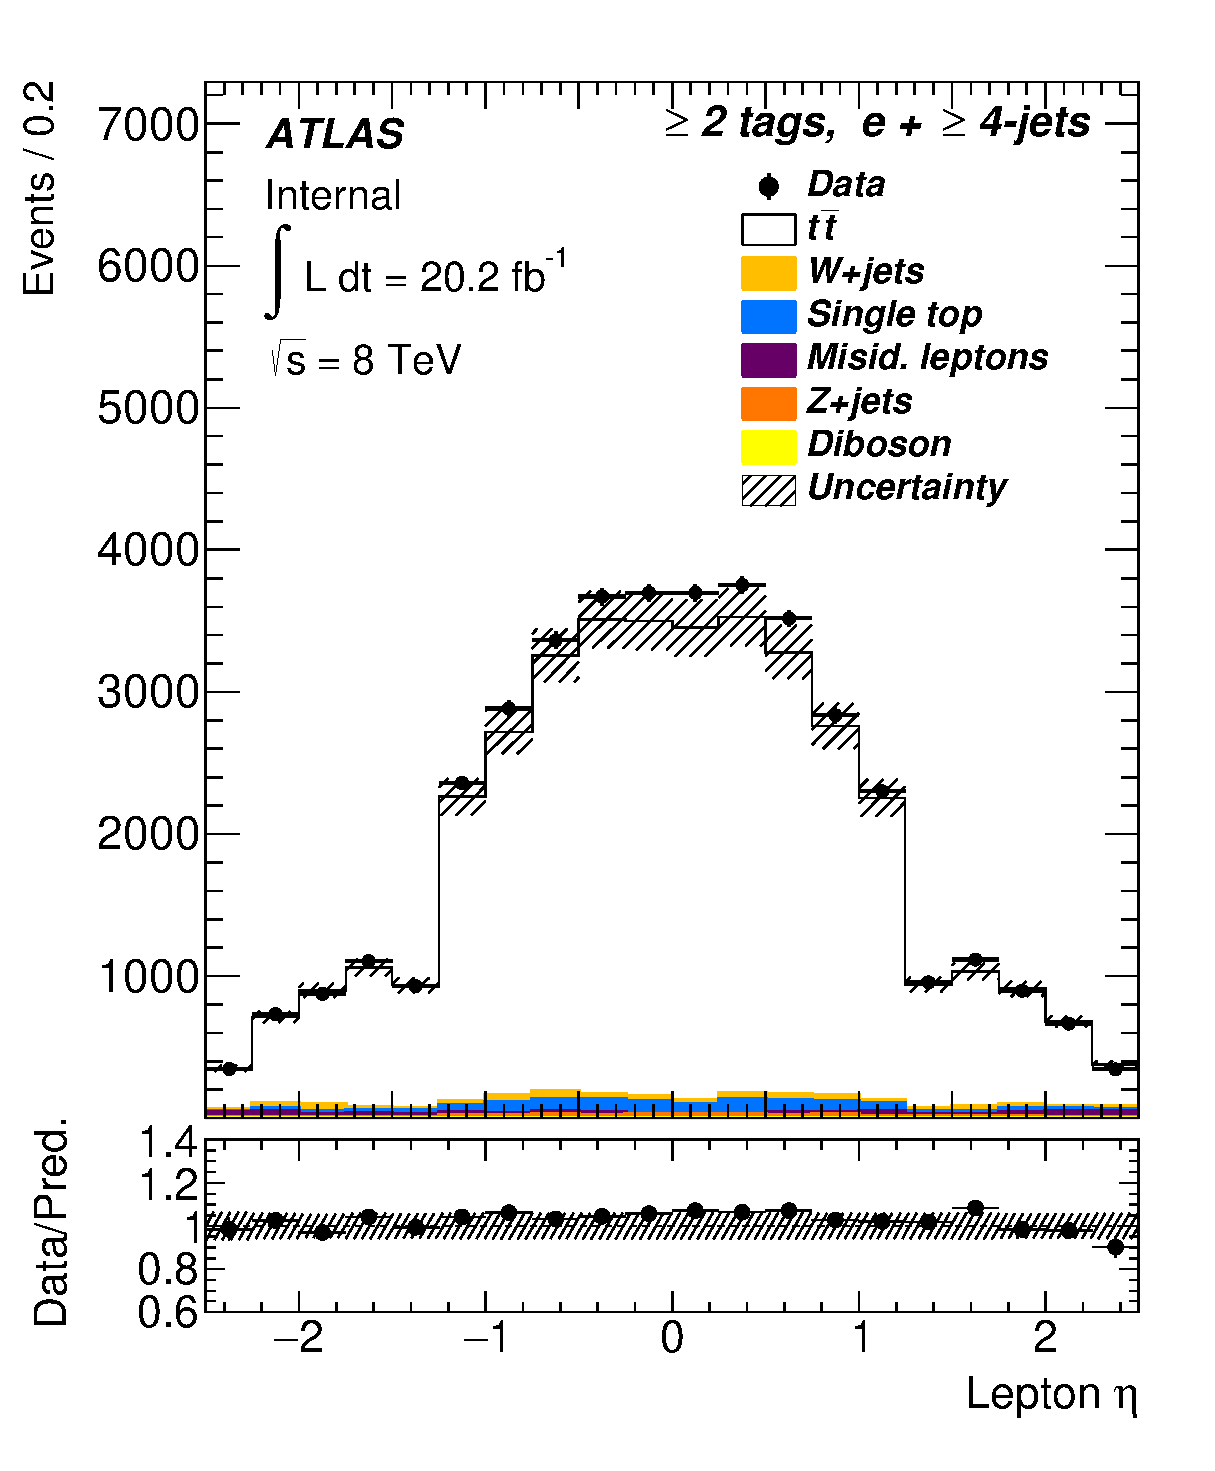
\includegraphics[width=.95\textwidth]{../chapters/whel/figures/control_Plots2/bTag_2incl/LeptonEta_el}\\
      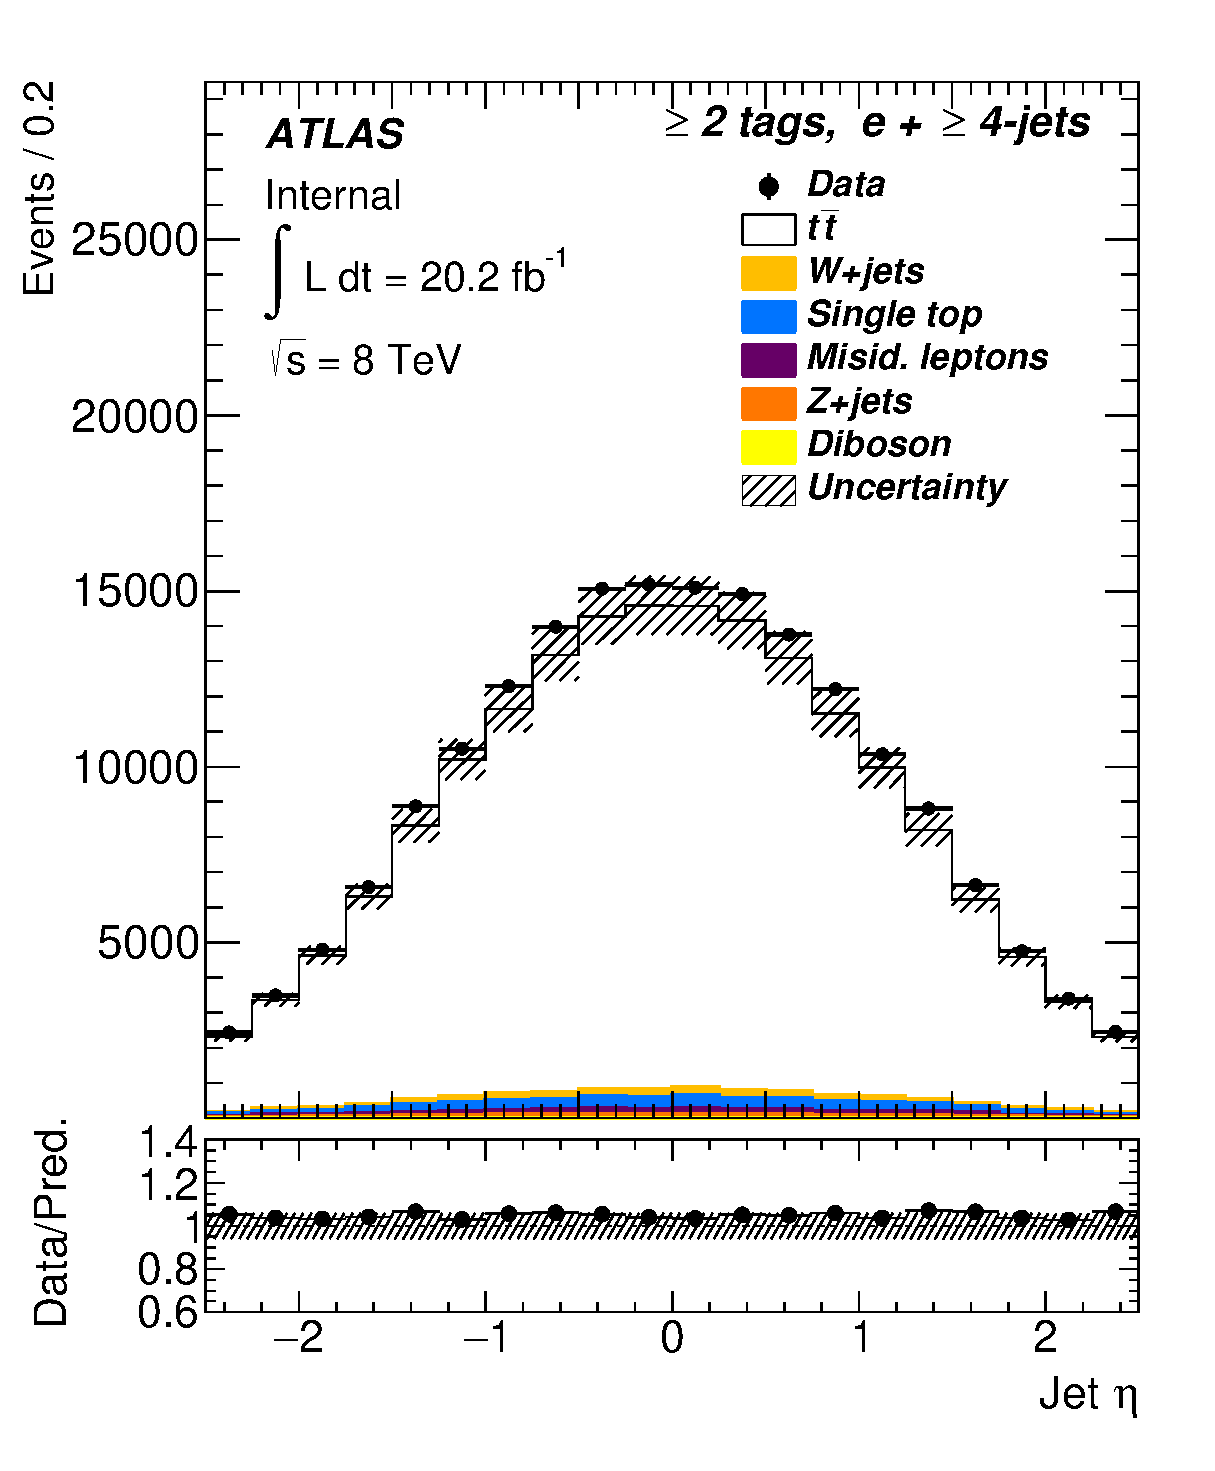
\includegraphics[width=.95\textwidth]{../chapters/whel/figures/control_Plots2/bTag_2incl/JetEta_el}
      \column{.333\textwidth}
      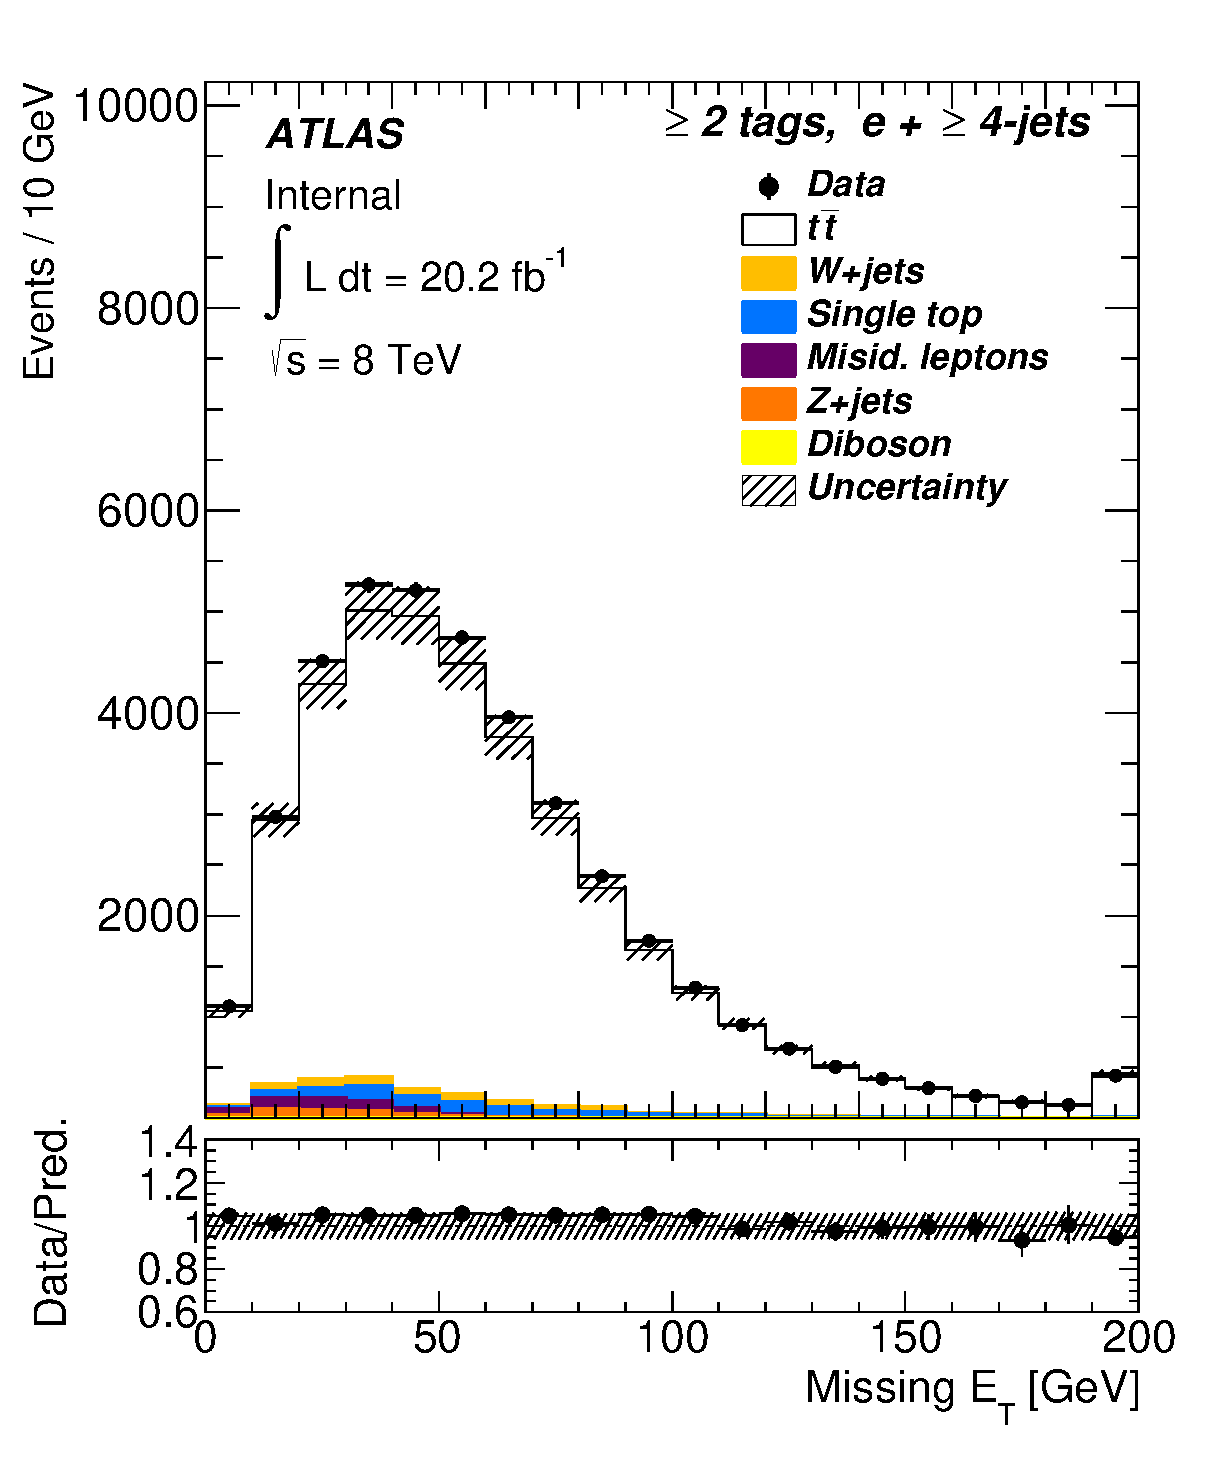
\includegraphics[width=.95\textwidth]{../chapters/whel/figures/control_Plots2/bTag_2incl/MissingEt_el}\\
      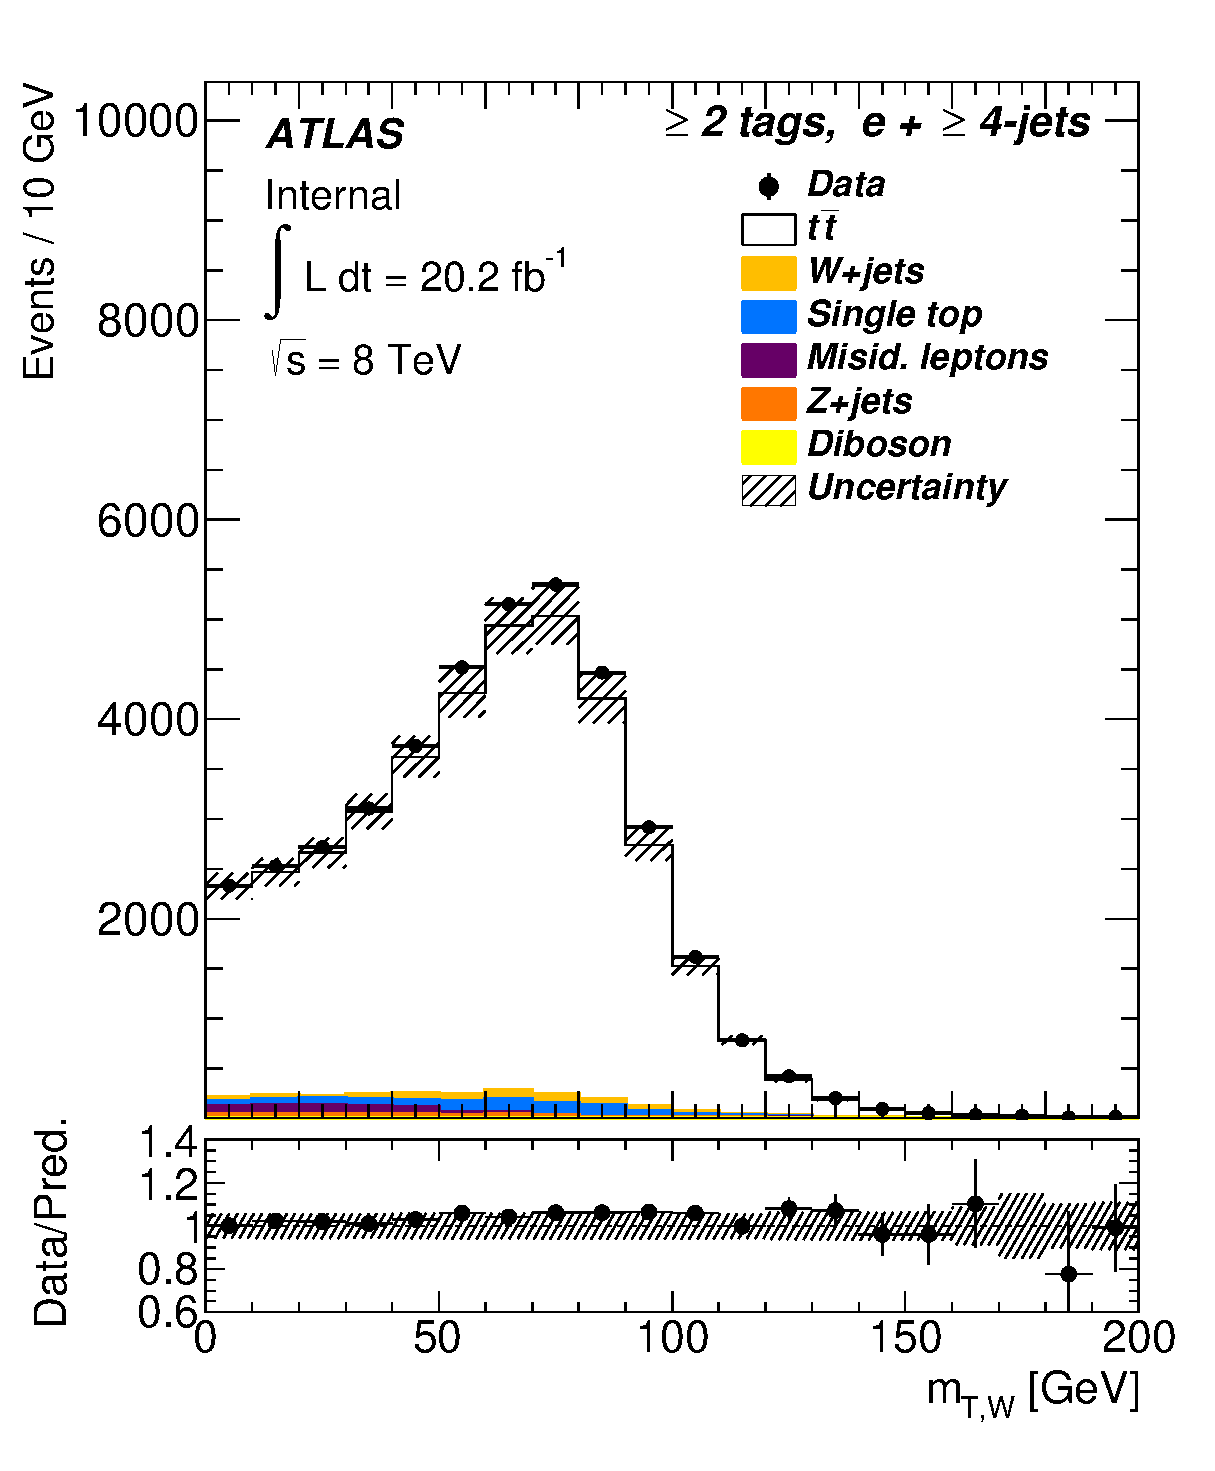
\includegraphics[width=.95\textwidth]{../chapters/whel/figures/control_Plots2/bTag_2incl/TransverseMass_el}
    \end{columns}
  \end{frame}

  \makeatletter % to change template
  \setbeamertemplate{headline}[default]
  \def\beamer@entrycode{\vspace*{-1.075\headheight}}
  \begin{frame}{Kinematic Distributions: Muon Channel, $\geq2\text{ } \lowercase{ b\text{-tags}}$}
    \vspace{5pt}
    \begin{columns}
      \column{.333\textwidth}
      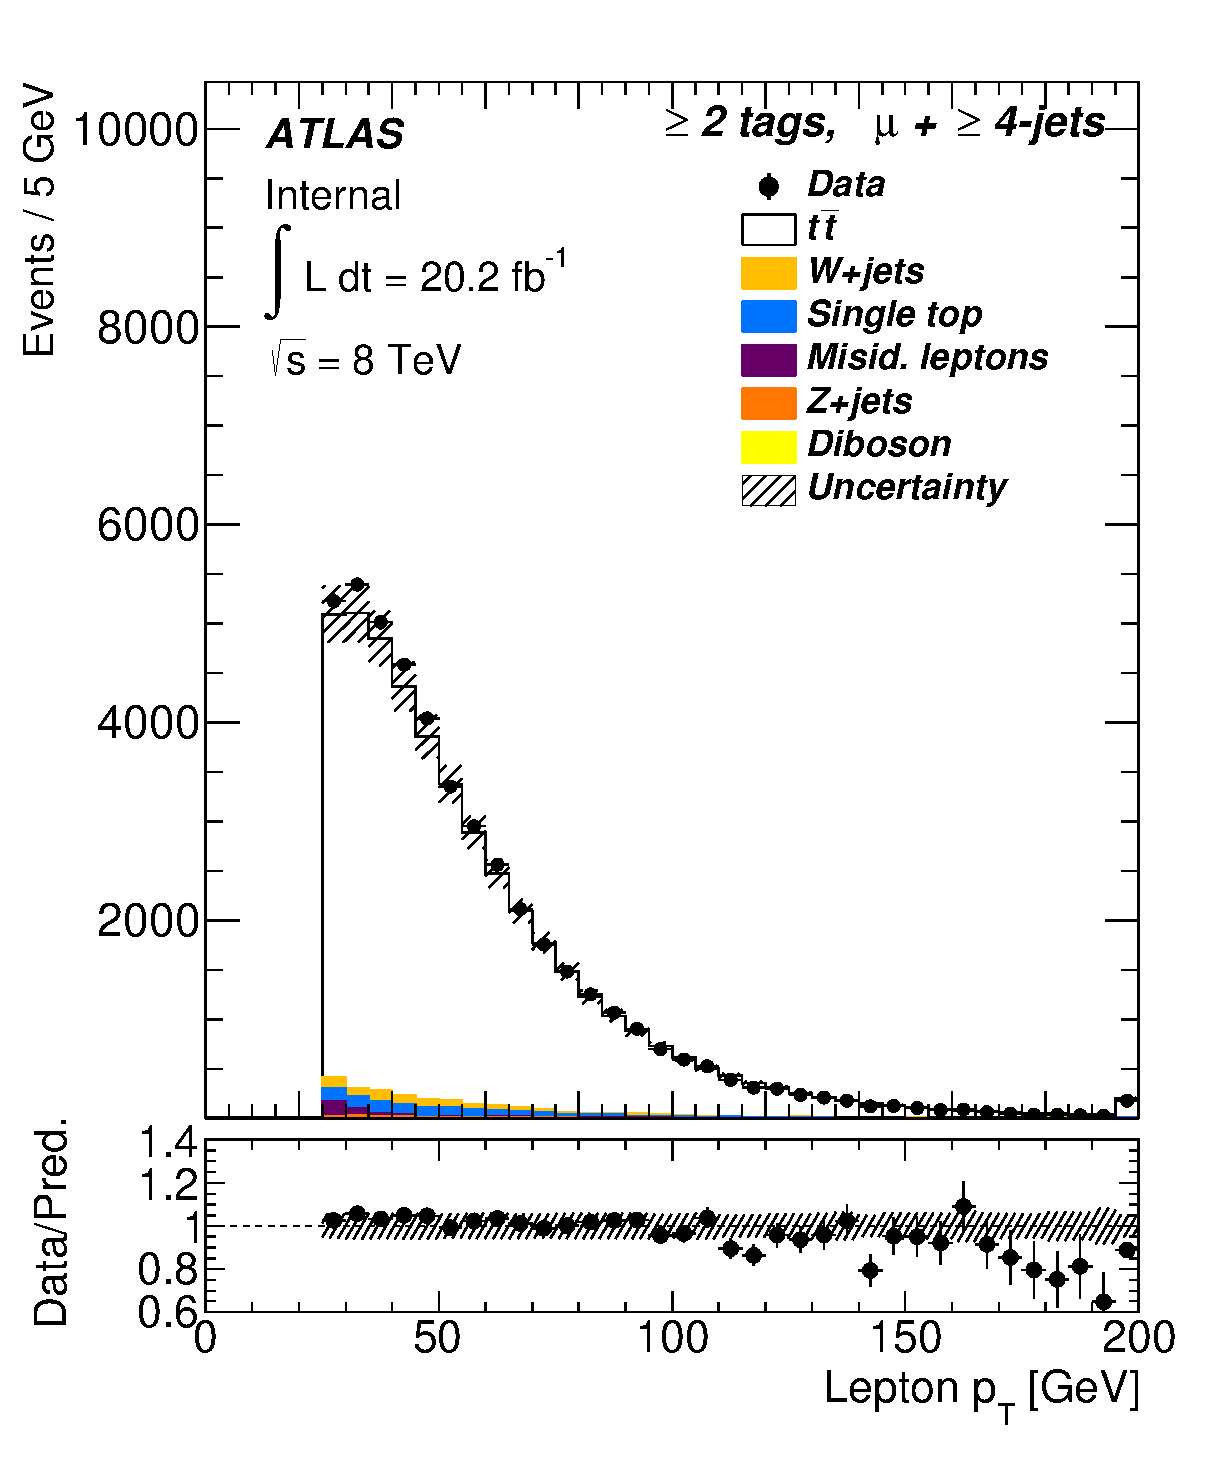
\includegraphics[width=.95\textwidth]{../chapters/whel/figures/control_Plots2/bTag_2incl/LeptonPt_mu}\\
      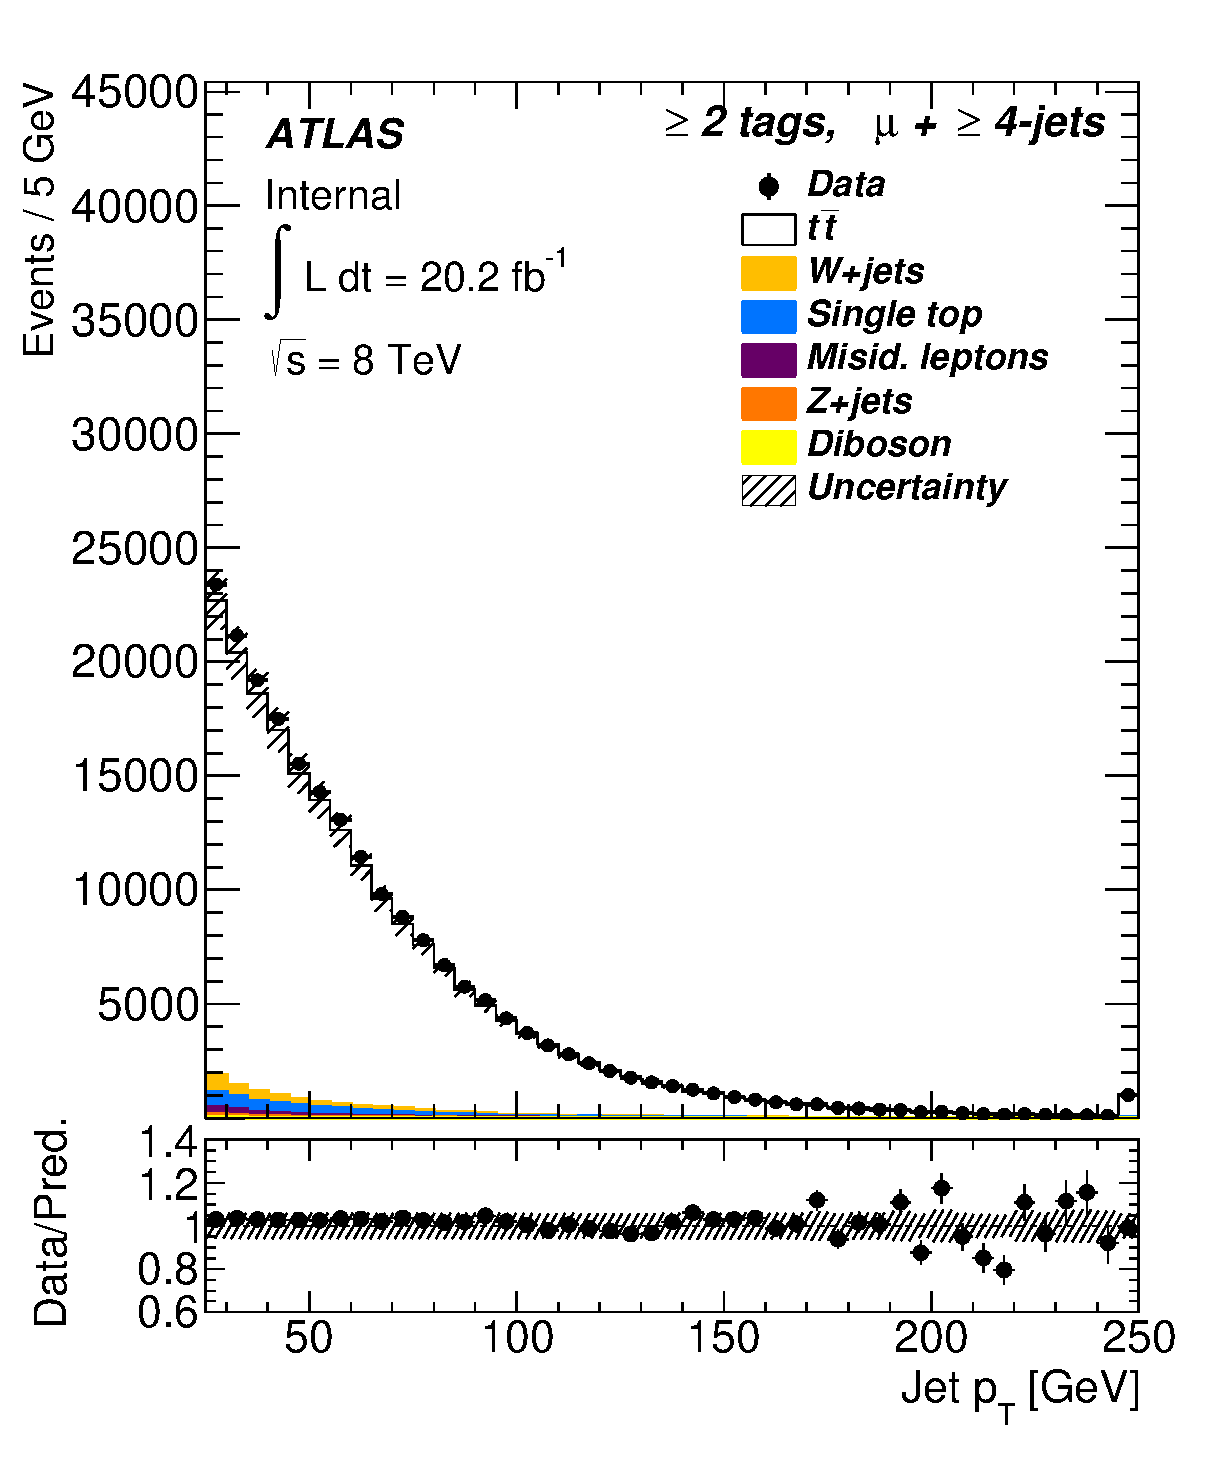
\includegraphics[width=.95\textwidth]{../chapters/whel/figures/control_Plots2/bTag_2incl/JetPt_mu}
      \column{.333\textwidth}
      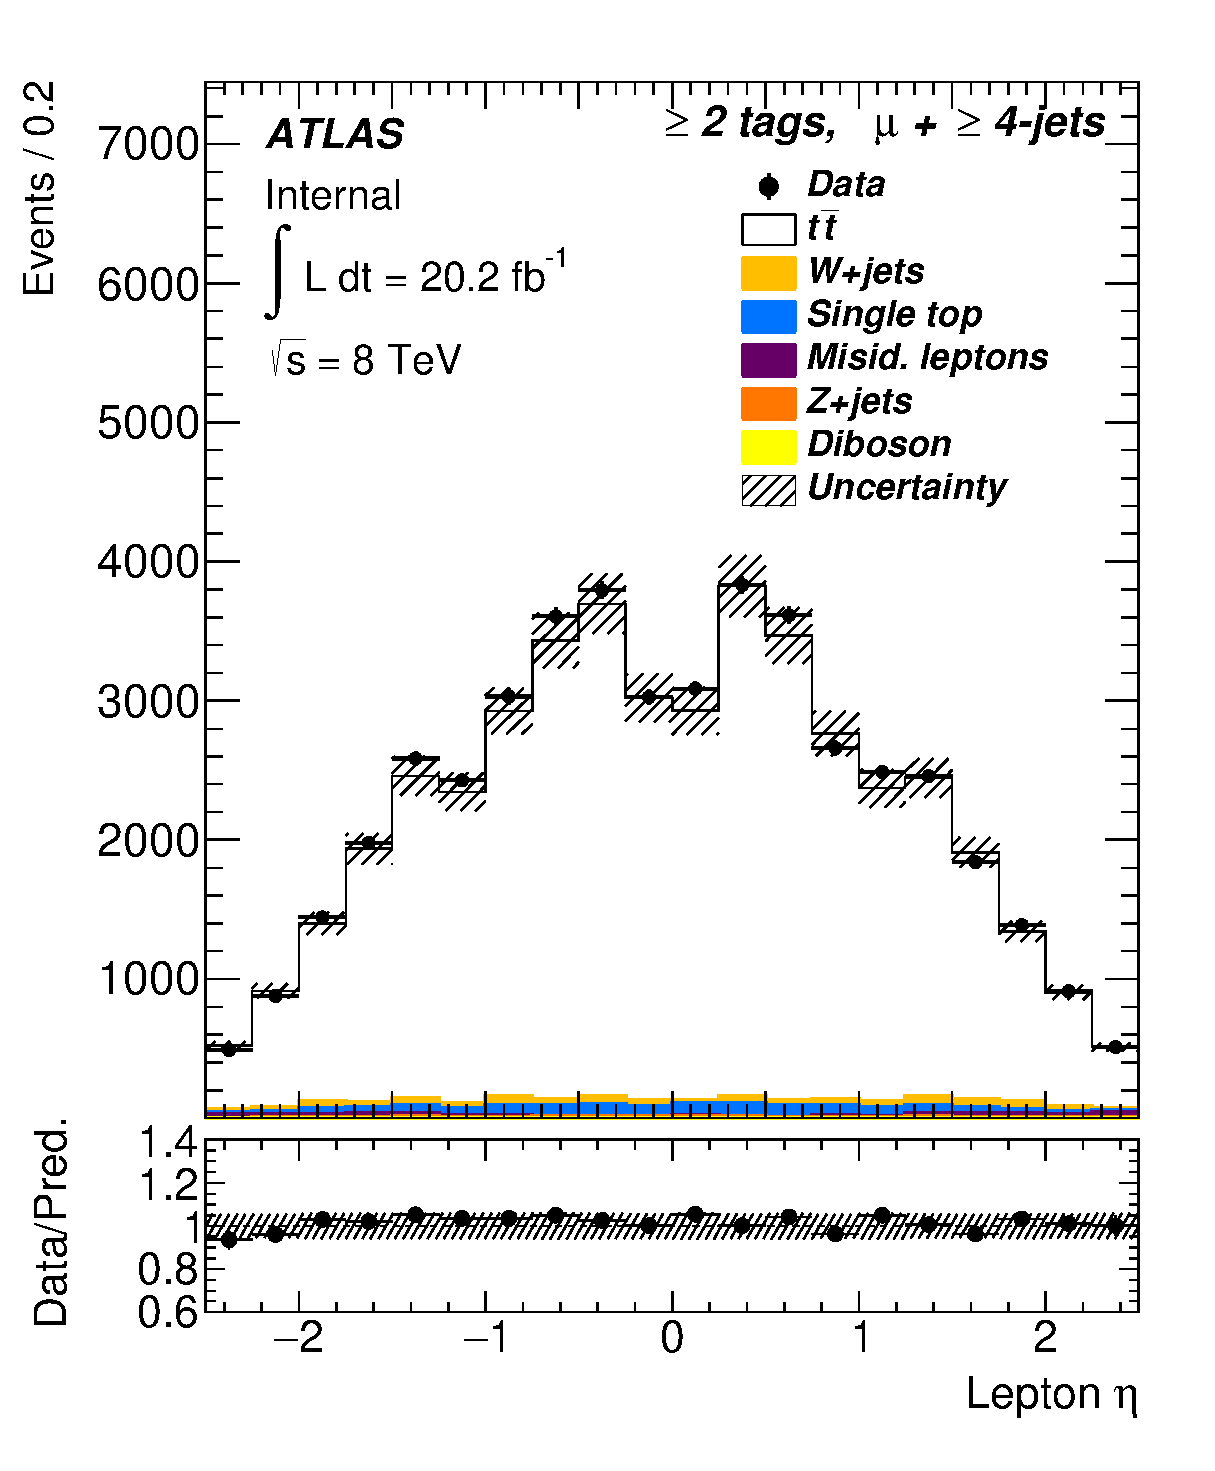
\includegraphics[width=.95\textwidth]{../chapters/whel/figures/control_Plots2/bTag_2incl/LeptonEta_mu}\\
      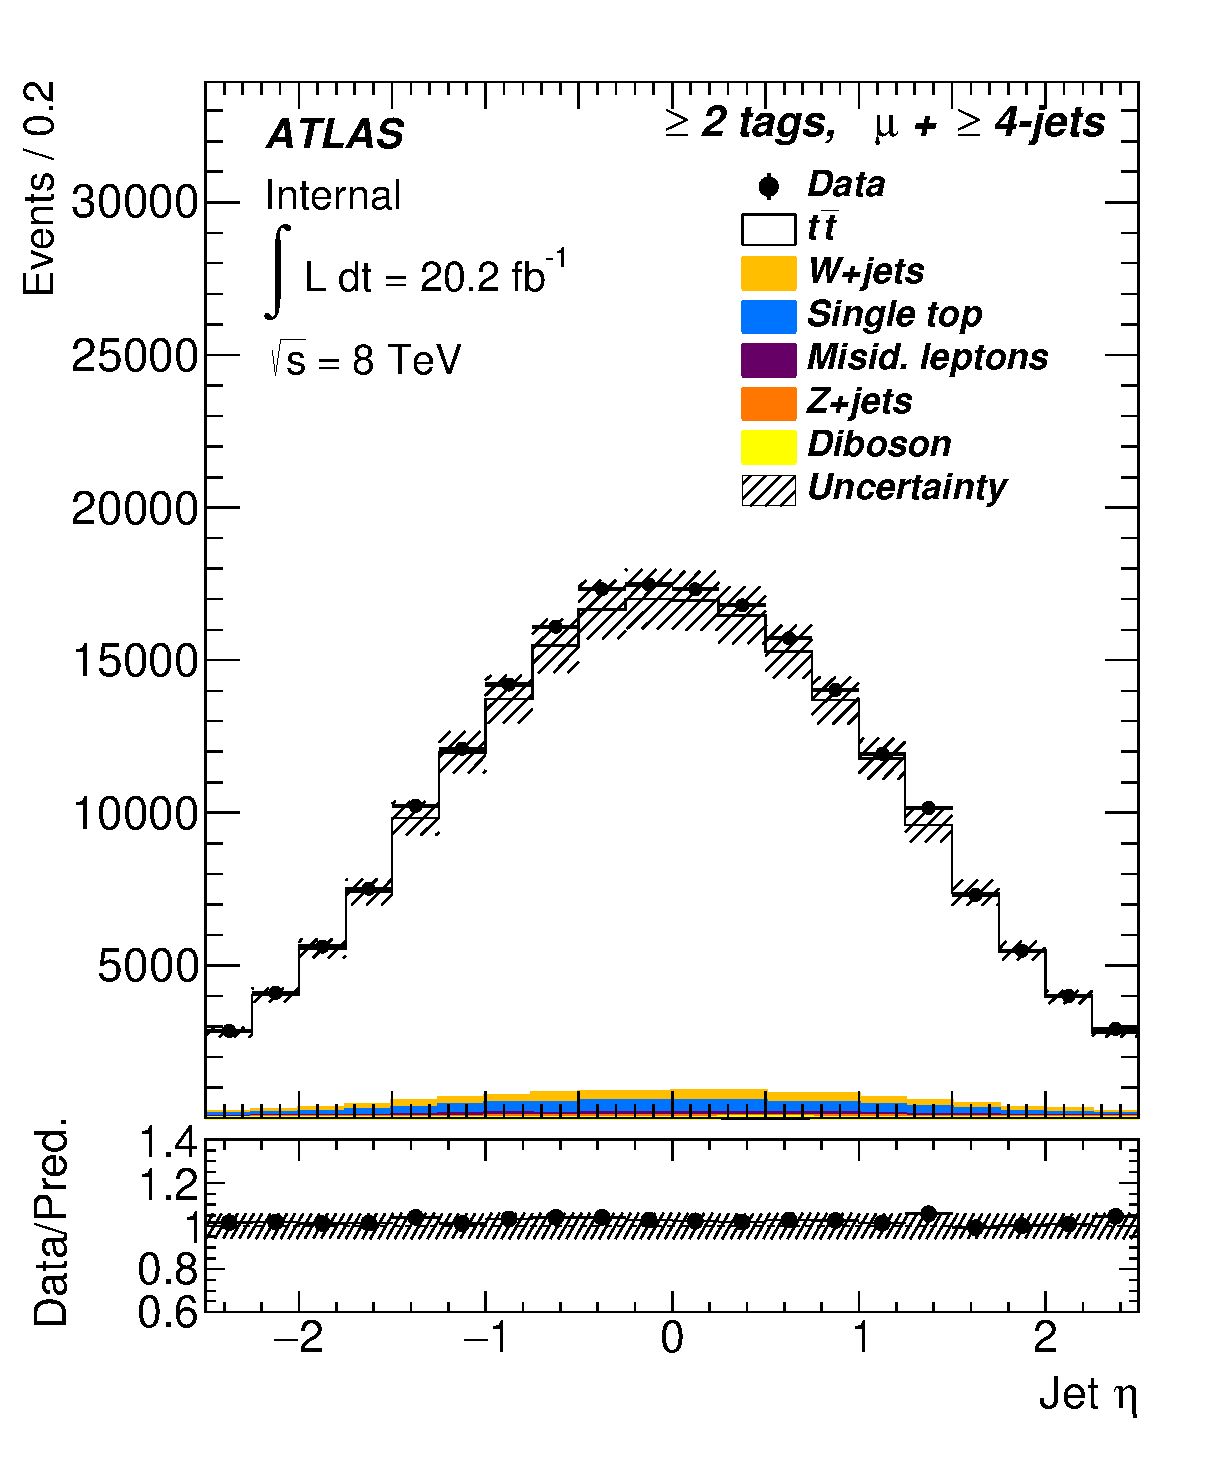
\includegraphics[width=.95\textwidth]{../chapters/whel/figures/control_Plots2/bTag_2incl/JetEta_mu}
      \column{.333\textwidth}
      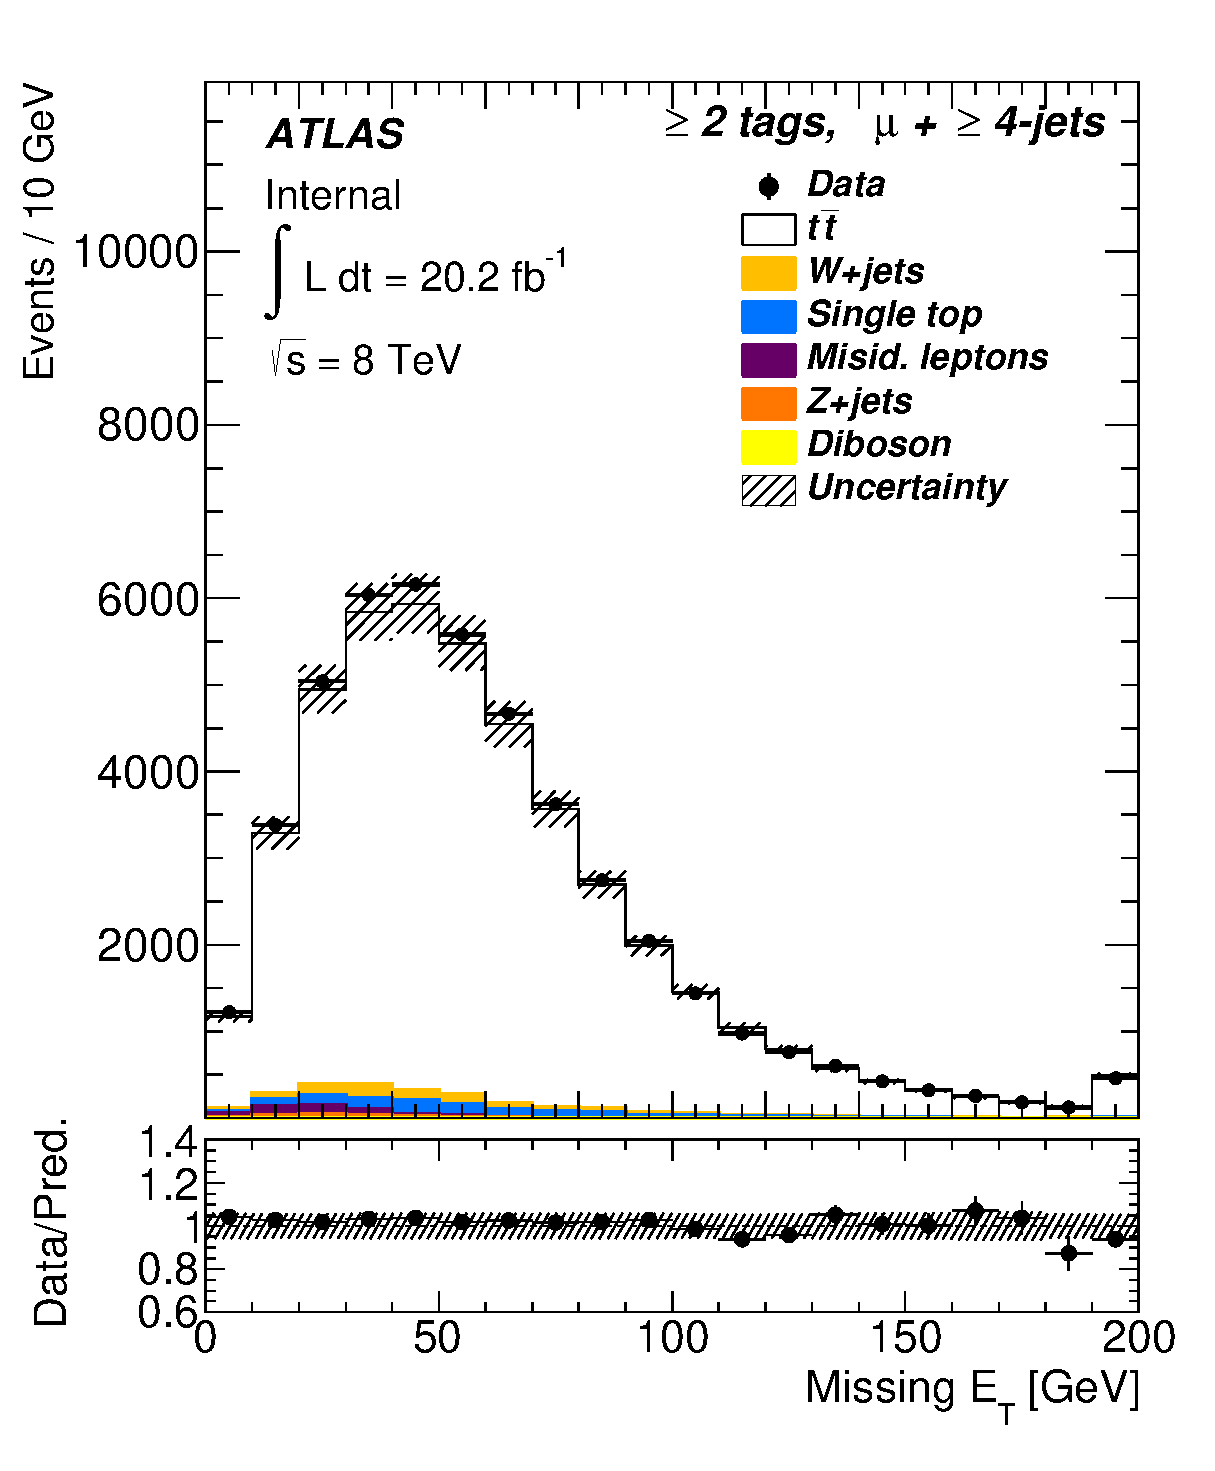
\includegraphics[width=.95\textwidth]{../chapters/whel/figures/control_Plots2/bTag_2incl/MissingEt_mu}\\
      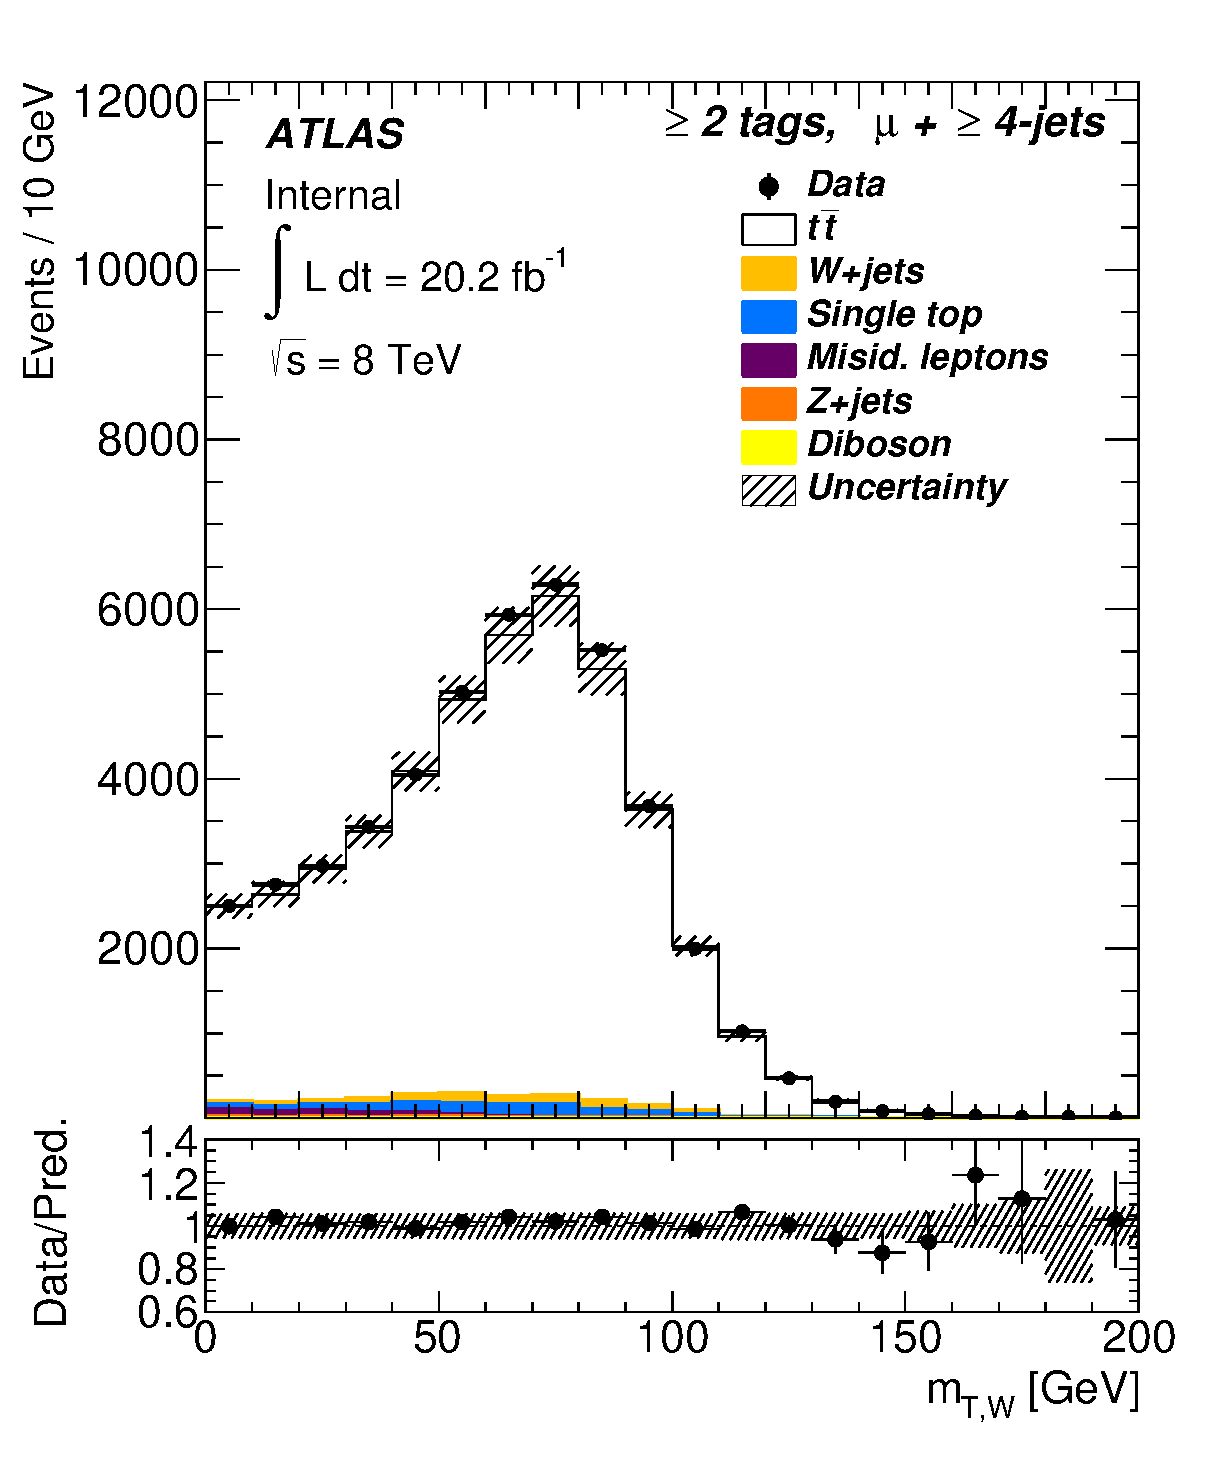
\includegraphics[width=.95\textwidth]{../chapters/whel/figures/control_Plots2/bTag_2incl/TransverseMass_mu}
    \end{columns}
  \end{frame}

  \makeatletter % to change template
  \setbeamertemplate{headline}[default]
  \def\beamer@entrycode{\vspace*{-1.075\headheight}}
  \begin{frame}{Kinematic Fitting I}
     \Wider{
      \begin{columns}
        \column{.5\textwidth}
        \begin{itemize}
          \footnotesize
        \item Permute two highest $b$-tagged jets + next three jets leading in p$_{T}$
        %\item Use kinematic fitting to reconstruct $t\bar{t}$ system
        \item Calculate permuation probability using kinematic likelihood and $b$-tagging/p$_{T}$ jet information to differentiate hadronic $W$ daughters
        \item Require LH > -48 for purity and take most probable permutation
        \end{itemize}
        \column{.5\textwidth}
        \includegraphics[width=.85\textwidth]{figures/whel/kinematicFitting/feynmanLines}
        %\vspace{-6pt}
        %\begin{itemize}
        %  \footnotesize
        %
        %\end{itemize}
      \end{columns}
     }
     \vspace{-14pt}
     \begin{columns}
       \column{.5\textwidth}
       \begin{center}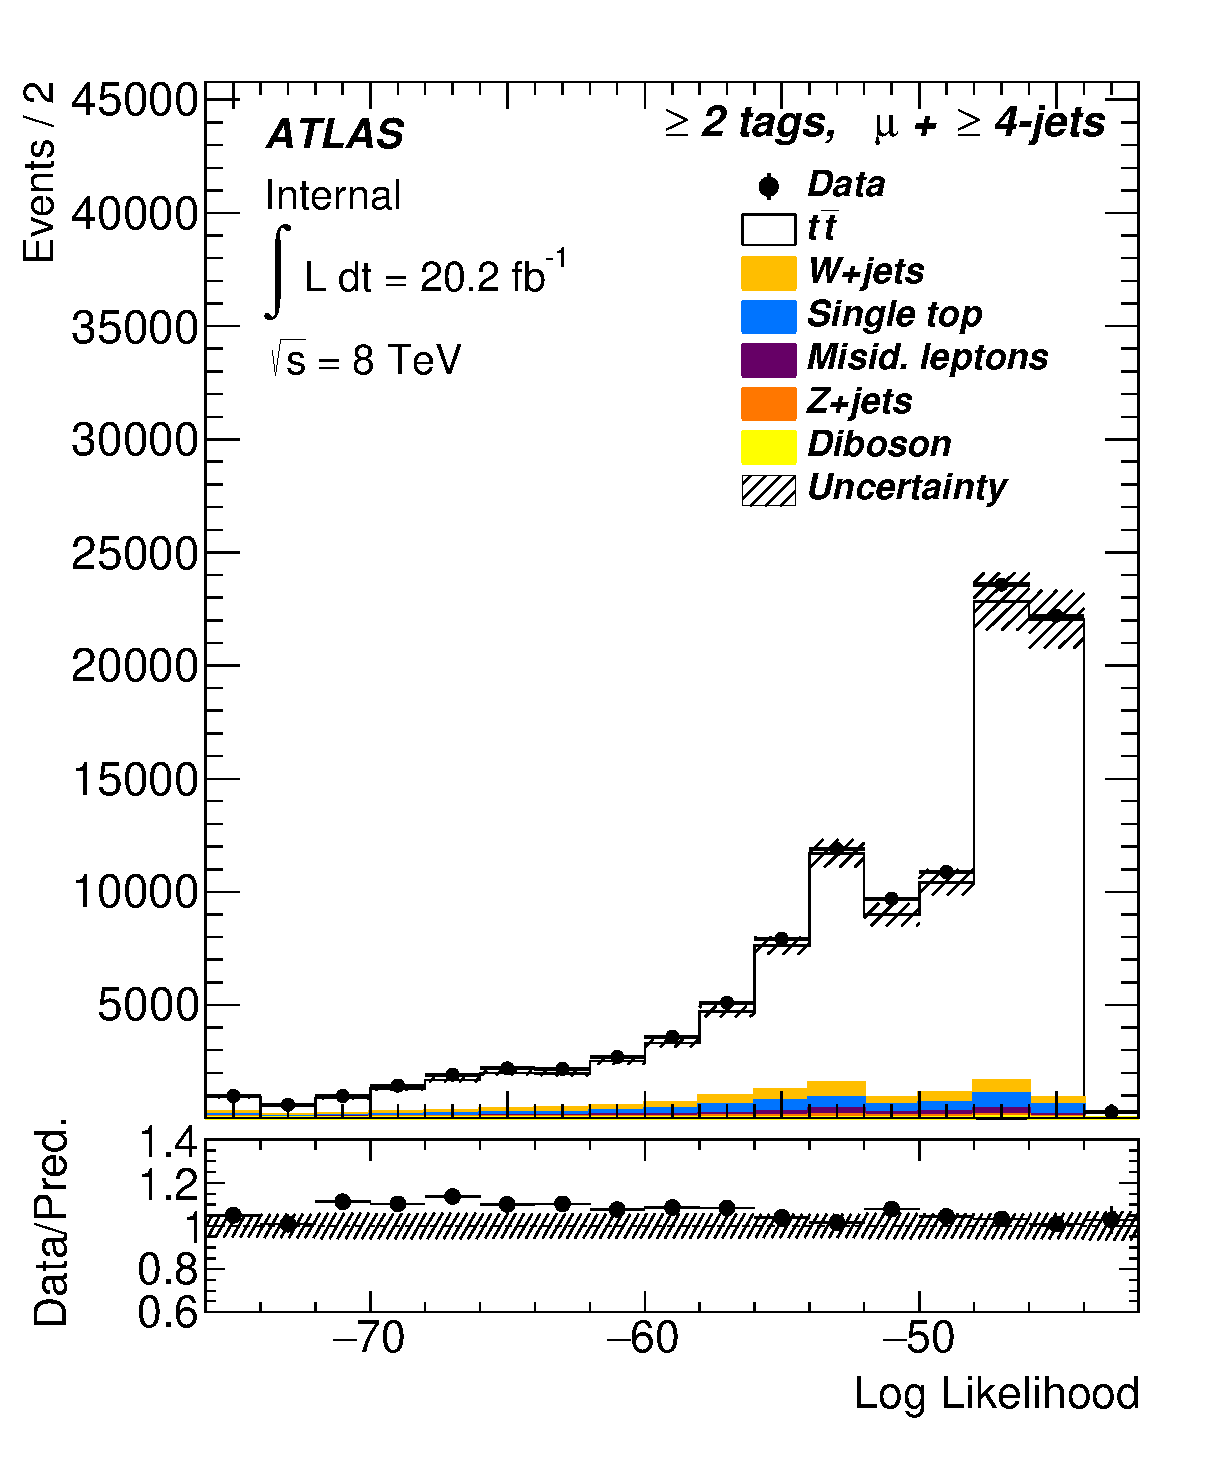
\includegraphics[width=.75\textwidth]{../chapters/whel/figures/control_Plots2/bTag_2incl_NoLHCut/LogLikelihood_mu}\end{center}
       \column{.5\textwidth}
       \begin{center}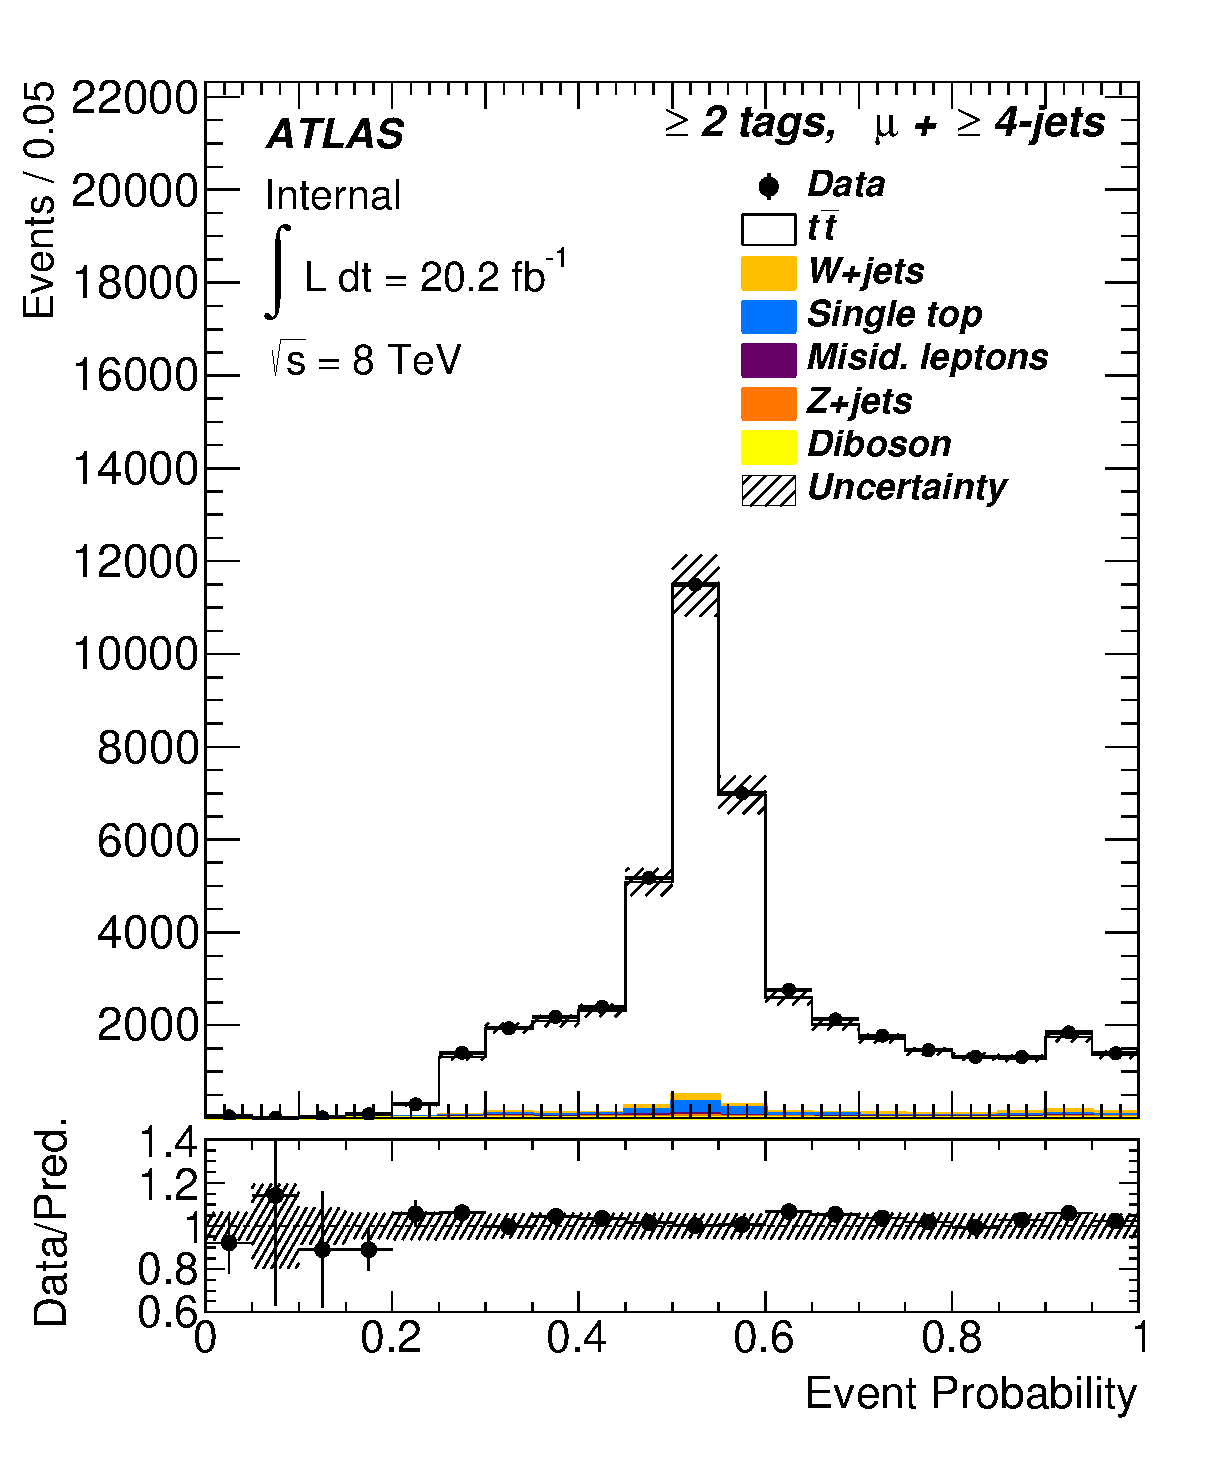
\includegraphics[width=.75\textwidth]{../chapters/whel/figures/control_Plots2/bTag_2incl/EventProbability_mu}\end{center}
     \end{columns}
  \end{frame}

  \makeatletter % to change template
  \setbeamertemplate{headline}[default]
  \def\beamer@entrycode{\vspace*{-1.075\headheight}}
  \begin{frame}{Kinematic Fitting II (U/D Separation)}
    \begin{center}
      \footnotesize
      $\mathcal{L}=\text{BW}(m_{q_1q_2q_3}| m_t\Gamma_{t})\cdot \text{BW}(m_{q_1q_2}| m_{W}\Gamma_{W})\cdot \text{BW}(m_{q_4\ell\nu}| m_t\Gamma_{t})\cdot \text{BW}(m_{\ell\nu} | m_W\Gamma_{W}) \nonumber$ \\
      $\prod\limits_{i=1}^4 W_{jet}(E_{i}^{meas}|E_{i})\cdot W_{\ell}(E_{\ell}^{meas}|E_{\ell})\cdot W_{miss}(E_{x}^{miss}|p_{x}^{\nu})\cdot W_{miss}(E_{y}^{miss}|p_{y}^{\nu})$
    \end{center}
    % \end{eqnarray}
    %\vspace{5pt}
    \begin{columns}
      \column{.5\textwidth}
      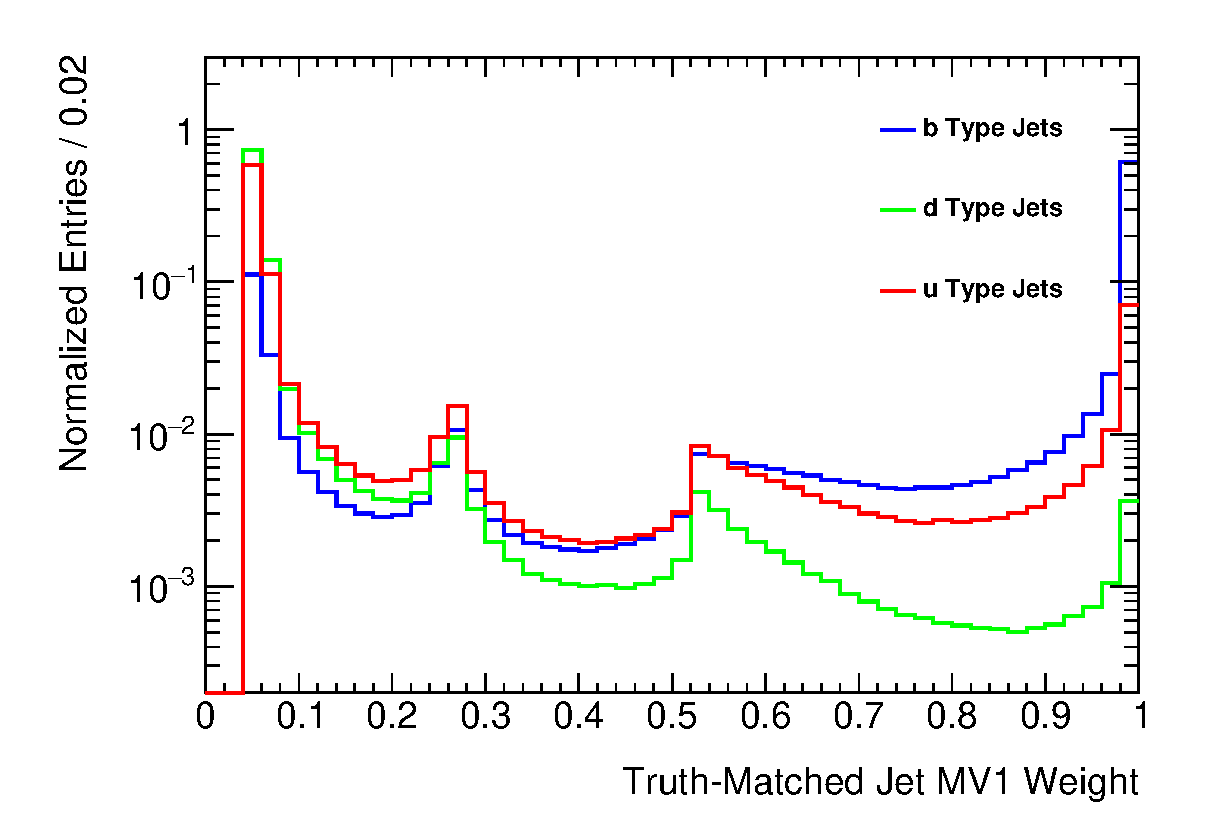
\includegraphics[width=\textwidth]{../chapters/whel/figures/mv1_template_5jetOPT}\\\vspace{-5pt}
      \column{.5\textwidth}
      \includegraphics[width=\textwidth]{../chapters/whel/figures/pt_template_5jetOPT}\\\vspace{-5pt}
    \end{columns}
    \begin{itemize}
      \footnotesize
    \item Kinematic likelihood extended to normalized event probability using jet p$_{T}$ and $b$-tag information
      \begin{eqnarray}
        p_{i}= \frac{\mathcal{L}_i\prod_j\Delta p_{i,j}}{\sum_i\mathcal{L}_i\prod_j\Delta p_{i,j}}
      \end{eqnarray}
      \vspace{2pt}
    \item $\Delta p_{i,j}$ calculated using unit normalized distributions of jet \pt MV1 weight
    \item Choose jet permutation with highest event probability
    %\item Cut on leading log likelihood to maximize sensitivity
    \end{itemize}
    
  \end{frame}

  \makeatletter % to change template
  \setbeamertemplate{headline}[default]
  \def\beamer@entrycode{\vspace*{-1.075\headheight}}
  \begin{frame}{Kinematic Fitting III (Optimizing Hadronic Sensitivity)}
    \vspace{3pt}
    \begin{columns}
      \column{.5\textwidth}
      \includegraphics[width=\textwidth]{../chapters/whel/figures/lh_stack}
      \column{.5\textwidth}
      \includegraphics[width=\textwidth]{../chapters/whel/figures/evProb_stack}
    \end{columns}
    \begin{columns}
      \column{.5\textwidth}
      \vspace{-5pt}
      \begin{itemize}\fontsize{7}{8}\selectfont
      \item \underline{Right}: All 4 jets uniquely truth-matchable, fed into fit, and correctly assigned in the leading permutation
      \item \underline{Wrong}: All 4 jets uniquely truth-matchable, fed into fit, but not correctly assigned in the leading permutation
      \item \underline{Non-reco}: Due to acceptance loss or non-unique matching, not all four jets from the hard \ttbar decay can  be matched to reconstructed objects
      \item \underline{Bkg}: Dileptonic or tauonic \ttbar decays where no true hadronic angle exists
      \end{itemize}
      \column{.5\textwidth}
    \begin{itemize}\small
      \item u/d flavor matching not 100\% efficient
      \item Selecting subset of events with correct reconstruction improves sensitivity of extracted helicity fractions
      \item Cut on LH $>$ -48 found to improve hadronic sensitivity and have negligible effect on leptonic sensitivity
    \end{itemize}
    \end{columns}
  \end{frame}

  \makeatletter % to change template
  \setbeamertemplate{headline}[default]
  \def\beamer@entrycode{\vspace*{-1.075\headheight}}
  \begin{frame}{$\lowercase{\text{cos}}~\theta^*$ Distributions, $=1\text{ } \lowercase{ b\text{-tag}}$}
    \begin{columns}
      \column{.5\textwidth}
      \includegraphics[width=\textwidth]{../chapters/whel/figures/control_Plots2/elmu_1excl_LH48/CosTheta_reco_lep_elmu}\\
      \vspace{-10pt}\begin{center}\textbf{Leptonic Angle}\end{center}
      \column{.5\textwidth}
      \includegraphics[width=\textwidth]{../chapters/whel/figures/control_Plots2/elmu_1excl_LH48/CosTheta_reco_had_elmu}\\
      \vspace{-10pt}\begin{center}\textbf{Hadronic Angle}\end{center}
    \end{columns}
  \end{frame}

  \makeatletter % to change template
  \setbeamertemplate{headline}[default]
  \def\beamer@entrycode{\vspace*{-1.075\headheight}}
  \begin{frame}{$\lowercase{\text{cos}}~\theta^*$ Distributions, $\geq2\text{ } \lowercase{ b\text{-tags}}$}
    \begin{columns}
      \column{.5\textwidth}
      \includegraphics[width=\textwidth]{../chapters/whel/figures/control_Plots2/elmu_2incl_LH48/CosTheta_reco_lep_elmu}\\
      \vspace{-10pt}\begin{center}\textbf{Leptonic Angle}\end{center}
      \column{.5\textwidth}
      \includegraphics[width=\textwidth]{../chapters/whel/figures/control_Plots2/elmu_2incl_LH48/CosTheta_reco_had_elmu}\\
      \vspace{-10pt}\begin{center}\textbf{Hadronic Angle}\end{center}
    \end{columns}
  \end{frame}

  \makeatletter % to change template
  \setbeamertemplate{headline}[default]
  \def\beamer@entrycode{\vspace*{-1.075\headheight}}
  \begin{frame}{Template Fitting: Pure Templates}
    \Wider{
      \begin{itemize}
        \small
      \item Reweight final reco distribution to produce templates for \fo, \fl, \fr
        \begin{itemize}
          \footnotesize
        \item Create templates for electron/muon channel, leptonic/hadronic angle, 1 exclusive + 2 inclusive $b$-tags
        \end{itemize}  \footnotesize
        %\vspace{5pt}
        \begin{equation*}
          W_i(\cos\theta^*) = \frac{w_i(\cos\theta^*)}{w_0(\cos\theta^*)+w_L(\cos\theta^*)+w_R(\cos\theta^*)}
        \end{equation*}
        where $i$ = 0, L, R and the components $w_i(\cos\theta^*)$ have functional form 
        \begin{equation*}
          w_0(\cos\theta^*) = \frac{3}{4}(1-cos^2\theta^*)\fo^{\text{MC}},\text{     } 
          w_L(\cos\theta^*) = \frac{3}{8}(1-cos\theta^*)^2\fl^{\text{MC}}
        \end{equation*}
        \vspace{-15pt}
        \begin{equation*}
          w_R(\cos\theta^*) = \frac{3}{8}(1+cos\theta^*)^2\fr^{\text{MC}}
        \end{equation*}
        
        % \item Final result obtained using electron and muon channel, leptonic angle, 2 inclusive $b$-tag region
      \end{itemize}
      %\vspace{5pt}
      \centering\small\underline{Electron channel}
      \vspace{-20pt}
      \begin{columns}
        %\column{.05\textwidth}
        \column{.317\textwidth}
        \begin{center}\includegraphics[width=1.16\textwidth]{../chapters/whel/figures/templatePlots/Leptonic/Signal_Templates_2incl_el_lep}\end{center}\vspace{-15pt}\centering\tiny
        \textbf{Leptonic, $\geq2$ $b$-tags}
        \column{.317\textwidth}
        \begin{center}\includegraphics[width=1.16\textwidth]{../chapters/whel/figures/templatePlots/Hadronic/Signal_Templates_2incl_el_had}\end{center}\vspace{-15pt}\centering\tiny
        \textbf{Hadronic, $\geq2$ $b$-tags}
        \column{.317\textwidth}
        \begin{center}\includegraphics[width=1.16\textwidth]{../chapters/whel/figures/templatePlots/Hadronic/Signal_Templates_1excl_el_had}\end{center}\vspace{-15pt}\centering\tiny
        \textbf{Hadronic, $=1$ $b$-tag}
        \column{.05\textwidth}
      \end{columns}
    }
  \end{frame}


  \makeatletter % to change template
  \setbeamertemplate{headline}[default]
  \def\beamer@entrycode{\vspace*{-1.075\headheight}}
  \begin{frame}[noframenumbering]{Template Fitting: Pure Templates}
    \Wider{
      \begin{itemize}
        \small
      \item Reweight final reco distribution to produce templates for \fo, \fl, \fr
        \begin{itemize}
          \footnotesize
        \item Create templates for electron/muon channel, leptonic/hadronic angle, 1 exclusive + 2 inclusive $b$-tags
        \end{itemize}  \footnotesize
        %\vspace{5pt}
        \begin{equation*}
          W_i(\cos\theta^*) = \frac{w_i(\cos\theta^*)}{w_0(\cos\theta^*)+w_L(\cos\theta^*)+w_R(\cos\theta^*)}
        \end{equation*}
        where $i$ = 0, L, R and the components $w_i(\cos\theta^*)$ have functional form 
        \begin{equation*}
          w_0(\cos\theta^*) = \frac{3}{4}(1-cos^2\theta^*)\fo^{\text{MC}},\text{     } 
          w_L(\cos\theta^*) = \frac{3}{8}(1-cos\theta^*)^2\fl^{\text{MC}}
        \end{equation*}
        \vspace{-15pt}
        \begin{equation*}
          w_R(\cos\theta^*) = \frac{3}{8}(1+cos\theta^*)^2\fr^{\text{MC}}
        \end{equation*}
        
        % \item Final result obtained using electron and muon channel, leptonic angle, 2 inclusive $b$-tag region
      \end{itemize}
      %\vspace{5pt}
      \centering\small\underline{Muon channel}
      \vspace{-20pt}
      \begin{columns}
        %\column{.05\textwidth}
        \column{.317\textwidth}
        \begin{center}\includegraphics[width=1.16\textwidth]{../chapters/whel/figures/templatePlots/Leptonic/Signal_Templates_2incl_mu_lep}\end{center}\vspace{-15pt}\centering\tiny
        \textbf{Leptonic, $\geq2$ $b$-tags}
        \column{.317\textwidth}
        \begin{center}\includegraphics[width=1.16\textwidth]{../chapters/whel/figures/templatePlots/Hadronic/Signal_Templates_2incl_mu_had}\end{center}\vspace{-15pt}\centering\tiny
        \textbf{Hadronic, $\geq2$ $b$-tags}
        \column{.317\textwidth}
        \begin{center}\includegraphics[width=1.16\textwidth]{../chapters/whel/figures/templatePlots/Hadronic/Signal_Templates_1excl_mu_had}\end{center}\vspace{-15pt}\centering\tiny
        \textbf{Hadronic, $=1$ $b$-tag}
        \column{.05\textwidth}
      \end{columns}
    }
  \end{frame}


  \makeatletter % to change template
  \setbeamertemplate{headline}[default]
  \def\beamer@entrycode{\vspace*{-1.075\headheight}}
  \begin{frame}[plain]{Template Fitting: Likelihood Fit}
    \Wider{
      \begin{itemize}\footnotesize
      \item Perform bin-by-bin likelihood fit to final $\cos\theta^*$ distribution
      \end{itemize}
      \vspace{-18pt}
      \footnotesize
      \begin{center}${\mathcal{L}}=\prod\limits_{i=1}^{N_{bins}} \textrm{Poisson}(n_{\textrm{data},i}, n_{\textrm{exp},i}) \prod\limits_{j=1}^{N_{bkg}}\frac{1}{\sqrt{2\pi}\sigma_{\textrm{bkg.j}}}e^{\frac{-(n_{\textrm{bkg.j}}-\hat n_{\textrm{bkg.j}})^2}{2\sigma ^{2}_{\textrm{bkg.j}}}}$\end{center}
      \vspace{-17pt}
      \begin{center}$n_{\textrm{exp}}= n_{\textrm{0, templ.}} + n_{\textrm{L, templ.}} +n_{\textrm{R, templ.}}+n_{\textrm{W+light}}+n_{\textrm{W+$c$}}+n_{\textrm{W+$bb/cc$}}+n_{\textrm{QCD}}+n_{\textrm{Rem.Bkg.}}$\end{center}
      \vspace{-13pt}
      \begin{itemize}\footnotesize
      \item Background normalizations constrained by Gaussian priors w/ width of expected uncertainty
      \item Normalization of each $W$ helicity template and overall $t\bar{t}$ yield allowed to float
      \item Final fractions extracted using sum of template yields for each helicity state
      \end{itemize}
      \vspace{-14pt}
      \begin{center}$N_{i}=  \epsilon_{\text{i}}\cdot n_{\textrm{i, templ.}} \text{ and } F_{\text{i}}= \frac{N_{i}}{N_{0}+N_{L}+N_{R}}  \textrm{ \quad for i= 0, L, R.}$\end{center}
      %\begin{center}\small and\end{center}
      %\begin{center}\large$F_{\text{i}}= \frac{N_{i}}{N_{0}+N_{L}+N_{R}}  \textrm{ \quad for i= 0, L, R.}$\end{center}
      \vspace{-11pt}
      \begin{columns}
        %\column{.01\textwidth}
      \column{.3\textwidth}
      \includegraphics[width=1.15\textwidth]{../chapters/whel/figures/cali_curves_June-1-2017/Calicurve_F0_el_mu}
      \column{.3\textwidth}
      \includegraphics[width=1.15\textwidth]{../chapters/whel/figures/cali_curves_June-1-2017/Calicurve_FL_el_mu}
      \column{.3\textwidth}
      \includegraphics[width=1.15\textwidth]{../chapters/whel/figures/cali_curves_June-1-2017/Calicurve_FR_el_mu}
      \end{columns}
    }
  \end{frame}

  \makeatletter % to change template
  \setbeamertemplate{headline}[default]
  \def\beamer@entrycode{\vspace*{-1.075\headheight}}
  \begin{frame}{Evaluating Systematic Uncertainties}
    \begin{columns}
      \column{.6\textwidth}
      \begin{table}
        \begin{center}\fontsize{7}{8}\selectfont
        \begin{tabular}{lcc}
          \hline\hline
          Systematic uncertainty & Type  & Components\\
          \hline
          Luminosity                  &  N & 1\\\hline\hline
          {\bf Physics Objects}                 &   & \\
          Electron                  &  S,N & 5 \\
          Muon                      &  S,N & 6 \\\hline
          Jet energy scale            & S,N & 26\\
          Jet vertex fraction         & S,N    & 1\\
          Jet energy resolution       & S,N & 1\\
          Jet reconstruction      & S,N & 1\\ \hline
          $b$ tagging efficiency      & S,N & 6\\
          $c$ tagging efficiency      & S,N & 4\\
          Light jet tagging efficiency    & S,N & 12\\ \hline\hline
          {\bf Background Model}                 &   & \\
          $W$+light/$c$/$bb/cc$ calibration      &  N & 3\\
          %$W$ p$_{T}$ reweighting     &  S,N & 1\\
          $Z$+jets normalization      &  N & 1\\
          %$Z$ p$_{T}$ reweighting     &  S,N & 1\\\hline
          Multijet normalization      &  N & 1\\
          %Multijet shape              &  S & 2\\
          \hline
          Single top cross section    &  N & 1\\
          %Single top model            &  S,N & 1\\
          Diboson+jets normalization  &  N & 1\\ \hline\hline
          {\bf Signal Model}                 &   & \\
          $t\bar{t}$ scale           & S,N & 2 \\
          $t\bar{t}$ generator       & S,N & 1 \\
          $t\bar{t}$ hadronization   & S,N & 1 \\
          $t\bar{t}$ PDF   & S,N & 1 \\
          $t\bar{t}$ modeling: parton shower & S,N & 1\\
          $t\bar{t}$ underlying events & S,N & 1\\
          \hline\hline
        \end{tabular}
        \end{center}       
      \end{table}
      \vspace{-10pt}
      \tiny *S type means uncertainty on the shape is considered, and N type signifies uncertainty is considered on the normalization.
      \column{.5\textwidth}
      \begin{itemize}
        \footnotesize
      \item Generate 5000 sets of pseudo-data for each systematic variation
      \item Perform likelihood fit using nominal templates and systematically varied pseudo-data
      \item Difference of Gaussian mean between nominal pseudo-data and varied pseudo-data taken as uncertainty in F$_i$ 
      \item Only keep systematics where difference between varied templates and nominal templates greater than MC stat. uncertainty of nominal
      \item Symmetrize individual components and sum all sources in quadrature to obtain final systematic error
      \end{itemize}
    \end{columns}


  \end{frame}

  \makeatletter % to change template
  \setbeamertemplate{headline}[default]
  \def\beamer@entrycode{\vspace*{-1.075\headheight}}
  \begin{frame}{Total Uncertainty: \fo}
    \begin{columns}
      \column{.6\textwidth}
      \vspace{-14pt}
      \begin{table}[h!]\fontsize{5}{6}\selectfont
        \centering
        
        \begin{tabular}{lcccc}
          \hline\hline
          \multicolumn{5}{c}{\fo}\\
          \hline
          Systematic uncertainty & N$_{syst}$ & Lep 2incl & Had 1excl+2incl & Lep+Had 1excl+2incl \\\hline
          \multicolumn{5}{c}{Reconstructed Objects} \\\hline
          \multirow{2}{*}{Muon} & \multirow{2}{*}{6(3)} & +0.0024 & +0.0026 & +0.0026\\
                                 &                       & -0.0029 & -0.0037 & -0.0026\\\hline
          \multirow{2}{*}{Electron} & \multirow{2}{*}{5(3)} & +0.0028 & +0.0025 & +0.0026\\
                                 &                       & -0.003 & -0.0021 & -0.003\\\hline
          \multirow{2}{*}{JES} & \multirow{2}{*}{26(6)} & +0.0063 & +0.0069 & +0.0077\\
                                 &                       & -0.0033 & -0.007 & -0.009\\\hline
          \multirow{2}{*}{JER} & \multirow{2}{*}{11(11)} & +0.0062 & +0.0274 & +0.0068\\
                                 &                       & -0.0059 & -0.031 & -0.0068\\\hline
          \multirow{2}{*}{JVF} & \multirow{2}{*}{1(1)} & +0.0036 & +0.0129 & +0.0025\\
                                 &                       & -0.0017 & -0.0092 & -0.0015\\\hline
          \multirow{2}{*}{\bt tagging} & \multirow{2}{*}{3(3)} & +0.0017 & +0.0289 & +0.0213\\
                                 &                       & -0.0021 & -0.0307 & -0.0211\\\hline
          
          \hline\hline
          \multirow{2}{*}{Sum of Reco Objects} & \multirow{2}{*}{-} & +0.0104 & +0.0426 & +0.0241\\
                                 &                       & -0.0084 & -0.0454 & -0.0243\\\hline
          
          \hline
          \multicolumn{5}{c}{Modeling} \\\hline
          \multirow{2}{*}{Radiation} & radLo & 0.0033 & 0.0178 & -0.0079\\
                                 & radHi & -0.0025 & -0.0108 & 0.0025\\ \hline
          \multirow{2}{*}{Parton Shower} & \multirow{2}{*}{1(1)} & +0.0019 & +0.015 & +0.0072\\
                                 &                       & -0.0019 & -0.015 & -0.0072\\\hline
          \multirow{2}{*}{ME Generator} & \multirow{2}{*}{1(1)} & +0.0025 & +0.0159 & +0.0019\\
                                 &                       & -0.0025 & -0.0159 & -0.0019\\\hline
          \multirow{2}{*}{PDF} & \multirow{2}{*}{3(3)} & +0.003 & +0.001 & +0.002\\
                                 &                       & -0.003 & -0.001 & -0.002\\\hline
          \multirow{2}{*}{Top Mass} & \multirow{2}{*}{3(3)} & +0.002 & +0.003 & +0.001\\
                                 &                       & -0.002 & -0.003 & -0.001\\\hline
          
          \hline\hline
          \multirow{2}{*}{Sum of Modeling} & \multirow{2}{*}{-} & +0.0058 & +0.0284 & +0.0111\\
                                 &                       & -0.0058 & -0.0284 & -0.0111\\\hline
          
          \hline
          \multicolumn{5}{c}{Method Uncertainty} \\\hline
          \multirow{2}{*}{Template Statistics} & \multirow{2}{*}{3(3)} & +0.009 & +0.008 & +0.005\\
                                 &                       & -0.009 & -0.008 & -0.005\\\hline
          
          \hline\hline
          \multirow{2}{*}{Total Syst.} & \multirow{2}{*}{-} & +0.0149 & +0.0518 & +0.027\\
                                 &                       & -0.0136 & -0.0541 & -0.0271\\\hline
          Stat. + Bkg. & - & 0.012 & 0.010 & 0.007 \\\hline
          
          \hline\hline
        \end{tabular}
        
      \end{table}
      \column{.4\textwidth}
      \begin{itemize}\footnotesize
        \item Numbers in parentheses in N$_{syst}$ column refer to the number of variations with systematic uncertainty larger than MC statistical uncertainty
        \item Single-sided sources of uncertainty are symmetrized
        \item For radiation uncertainty, the larger of the two variations is kept and symmetrized
        \item  When difference between total up and down systematic uncertainty is $<$ 0.015, magnitude of the larger uncertainty is taken as the total uncertainty
      \end{itemize}
    \end{columns}
    
  \end{frame}


  \makeatletter % to change template
  \setbeamertemplate{headline}[default]
  \def\beamer@entrycode{\vspace*{-1.075\headheight}}
  \begin{frame}{Total Uncertainty: \fl}
    \begin{columns}
      \column{.6\textwidth}
      \vspace{-14pt}
      \begin{table}[h!]\fontsize{5}{6}\selectfont
        \centering
        
        \begin{tabular}{lcccc}
          \hline\hline
          \multicolumn{5}{c}{\fl}\\
          \hline
          Systematic uncertainty & N$_{syst}$ & Lep 2incl & Had 1excl+2incl & Lep+Had 1excl+2incl \\\hline
          \multicolumn{5}{c}{Reconstructed Objects} \\\hline
          \multirow{2}{*}{Muon} & \multirow{2}{*}{6(3)} & +0.0013 & +0.0046 & +0.0011\\
                                 &                       & -0.0015 & -0.0035 & -0.0008\\\hline
          \multirow{2}{*}{Electron} & \multirow{2}{*}{5(3)} & +0.0018 & +0.0028 & +0.0011\\
                                 &                       & -0.002 & -0.0038 & -0.0014\\\hline
          \multirow{2}{*}{JES} & \multirow{2}{*}{26(6)} & +0.0028 & +0.0119 & +0.0022\\
                                 &                       & -0.0025 & -0.0078 & -0.0032\\\hline
          \multirow{2}{*}{JER} & \multirow{2}{*}{11(11)} & +0.0048 & +0.0329 & +0.0043\\
                                 &                       & -0.0018 & -0.0407 & -0.0019\\\hline
          \multirow{2}{*}{JVF} & \multirow{2}{*}{1(1)} & +0.0019 & +0.0012 & +0.0021\\
                                 &                       & -0.0013 & -0.0046 & -0.0017\\\hline
          \multirow{2}{*}{\bt tagging} & \multirow{2}{*}{3(3)} & +0.0012 & +0.0132 & +0.0082\\
                                 &                       & -0.0013 & -0.0143 & -0.0078\\\hline
          
          \hline\hline
          \multirow{2}{*}{Sum of Reco Objects} & \multirow{2}{*}{-} & +0.0064 & +0.0378 & +0.0099\\
                                 &                       & -0.0044 & -0.0444 & -0.009\\\hline
          
          \hline
          \multicolumn{5}{c}{Modeling} \\\hline
          \multirow{2}{*}{Radiation} & radLo & -0.0032 & 0.0393 & -0.006\\
                                 & radHi & 0.0058 & -0.0115 & 0.0076\\ \hline
          \multirow{2}{*}{Parton Shower} & \multirow{2}{*}{1(1)} & +0.0019 & +0.001 & +0.0086\\
                                 &                       & -0.0019 & -0.001 & -0.0086\\\hline
          \multirow{2}{*}{ME Generator} & \multirow{2}{*}{1(1)} & +0.0032 & +0.0242 & +0.0016\\
                                 &                       & -0.0032 & -0.0242 & -0.0016\\\hline
          \multirow{2}{*}{PDF} & \multirow{2}{*}{3(3)} & +0.003 & +0.001 & +0.002\\
                                 &                       & -0.003 & -0.001 & -0.002\\\hline
          \multirow{2}{*}{Top Mass} & \multirow{2}{*}{3(3)} & +0.002 & +0.003 & +0.001\\
                                 &                       & -0.002 & -0.003 & -0.001\\\hline
          
          \hline\hline
          \multirow{2}{*}{Sum of Modeling} & \multirow{2}{*}{-} & +0.0078 & +0.0463 & +0.0118\\
                                 &                       & -0.0078 & -0.0463 & -0.0118\\\hline
          
          \hline
          \multicolumn{5}{c}{Method Uncertainty} \\\hline
          \multirow{2}{*}{Template Statistics} & \multirow{2}{*}{3(3)} & +0.006 & +0.016 & +0.004\\
                                 &                       & -0.006 & -0.016 & -0.004\\\hline
          
          \hline\hline
          \multirow{2}{*}{Total Syst.} & \multirow{2}{*}{-} & +0.0135 & +0.0603 & +0.0162\\
                                 &                       & -0.0127 & -0.0646 & -0.0157\\\hline
          Stat. + Bkg. & - & 0.008 & 0.021 & 0.005 \\\hline
          
          \hline\hline
        \end{tabular}
        
      \end{table}
      \column{.4\textwidth}
      \begin{itemize}\footnotesize
        \item Numbers in parentheses in N$_{syst}$ column refer to the number of variations with systematic uncertainty larger than MC statistical uncertainty
        \item Single-sided sources of uncertainty are symmetrized
        \item For radiation uncertainty, the larger of the two variations is kept and symmetrized
        \item  When difference between total up and down systematic uncertainty is $<$ 0.015, magnitude of the larger uncertainty is taken as the total uncertainty
      \end{itemize}
    \end{columns}
    
  \end{frame}


  \makeatletter % to change template
  \setbeamertemplate{headline}[default]
  \def\beamer@entrycode{\vspace*{-1.075\headheight}}
  \begin{frame}{Total Uncertainty: \fr}
    \begin{columns}
      \column{.6\textwidth}
      \vspace{-14pt}
      \begin{table}[h!]\fontsize{5}{6}\selectfont
        \centering
        
        \begin{tabular}{lcccc}
          \hline\hline
          \multicolumn{5}{c}{\fr}\\
          \hline
          Systematic uncertainty & N$_{syst}$ & Lep 2incl & Had 1excl+2incl & Lep+Had 1excl+2incl \\\hline
          \multicolumn{5}{c}{Reconstructed Objects} \\\hline
          \multirow{2}{*}{Muon} & \multirow{2}{*}{6(3)} & +0.001 & +0.0072 & +0.0015\\
                                 &                       & -0.0015 & -0.0072 & -0.0017\\\hline
          \multirow{2}{*}{Electron} & \multirow{2}{*}{5(3)} & +0.0011 & +0.0051 & +0.0015\\
                                 &                       & -0.0011 & -0.0058 & -0.0017\\\hline
          \multirow{2}{*}{JES} & \multirow{2}{*}{26(6)} & +0.0037 & +0.0139 & +0.0073\\
                                 &                       & -0.0014 & -0.0054 & -0.0061\\\hline
          \multirow{2}{*}{JER} & \multirow{2}{*}{11(11)} & +0.0072 & +0.0573 & +0.0076\\
                                 &                       & -0.0067 & -0.0707 & -0.0065\\\hline
          \multirow{2}{*}{JVF} & \multirow{2}{*}{1(1)} & +0.0017 & +0.0114 & +0.0003\\
                                 &                       & -0.0006 & -0.0045 & -0.0002\\\hline
          \multirow{2}{*}{\bt tagging} & \multirow{2}{*}{3(3)} & +0.0011 & +0.0336 & +0.0132\\
                                 &                       & -0.0012 & -0.0349 & -0.0132\\\hline
          
          \hline\hline
          \multirow{2}{*}{Sum of Reco Objects} & \multirow{2}{*}{-} & +0.0085 & +0.0694 & +0.017\\
                                 &                       & -0.0072 & -0.0797 & -0.0161\\\hline
          
          \hline
          \multicolumn{5}{c}{Modeling} \\\hline
          \multirow{2}{*}{Radiation} & radLo & -0.0001 & -0.0573 & 0.014\\
                                 & radHi & -0.0034 & 0.022 & -0.0101\\ \hline
          \multirow{2}{*}{Parton Shower} & \multirow{2}{*}{1(1)} & +0.0037 & +0.0144 & +0.0013\\
                                 &                       & -0.0037 & -0.0144 & -0.0013\\\hline
          \multirow{2}{*}{ME Generator} & \multirow{2}{*}{1(1)} & +0.0057 & +0.0401 & +0.0033\\
                                 &                       & -0.0057 & -0.0401 & -0.0033\\\hline
          \multirow{2}{*}{PDF} & \multirow{2}{*}{3(3)} & +0.003 & +0.001 & +0.002\\
                                 &                       & -0.003 & -0.001 & -0.002\\\hline
          \multirow{2}{*}{Top Mass} & \multirow{2}{*}{3(3)} & +0.002 & +0.003 & +0.001\\
                                 &                       & -0.002 & -0.003 & -0.001\\\hline
          
          \hline\hline
          \multirow{2}{*}{Sum of Modeling} & \multirow{2}{*}{-} & +0.0084 & +0.0715 & +0.0146\\
                                 &                       & -0.0084 & -0.0715 & -0.0146\\\hline
          
          \hline
          \multicolumn{5}{c}{Method Uncertainty} \\\hline
          \multirow{2}{*}{Template Statistics} & \multirow{2}{*}{3(3)} & +0.004 & +0.016 & +0.003\\
                                 &                       & -0.004 & -0.016 & -0.003\\\hline
          
          \hline\hline
          \multirow{2}{*}{Total Syst.} & \multirow{2}{*}{-} & +0.0149 & +0.0999 & +0.023\\
                                 &                       & -0.0142 & -0.1074 & -0.0223\\\hline
          Stat. + Bkg. & - & 0.006 & 0.022 & 0.004 \\\hline
          
          \hline\hline
        \end{tabular}
      \end{table}
      \column{.4\textwidth}
      \begin{itemize}\footnotesize
        \item Numbers in parentheses in N$_{syst}$ column refer to the number of variations with systematic uncertainty larger than MC statistical uncertainty
        \item Single-sided sources of uncertainty are symmetrized
        \item For radiation uncertainty, the larger of the two variations is kept and symmetrized
        \item  When difference between total up and down systematic uncertainty is $<$ 0.015, magnitude of the larger uncertainty is taken as the total uncertainty
      \end{itemize}
    \end{columns}
    
  \end{frame}


  \makeatletter % to change template
  \setbeamertemplate{headline}[default]
  \def\beamer@entrycode{\vspace*{-1.075\headheight}}
  \begin{frame}{Helicity Fraction Results}
    \Wider{
      \begin{columns}
        \column{.46\textwidth}
        \begin{turn}{270}\includegraphics[height=70mm]{../chapters/whel/figures/results/Datafit_StatUnc_el_mu_lep2incl}\end{turn}
        \begin{turn}{270}\includegraphics[height=70mm]{../chapters/whel/figures/results/bTag_1excl2incl/Datafit_StatUnc_el_mu_bTag_had}\end{turn} 
        \column{.01\textwidth}
        \column{.48\textwidth}
        \begin{center}\fontsize{8}{9}\selectfont
          \begin{tabular}{l}
            \hline
            % \hline
            \multicolumn{1}{c}{Leptonic, $\geq$2 $b$-tags, $e+\mu$ Combination}\\%[5pt]
            \hline%\\%[1pt]
            \fo = 0.709 $\pm$ 0.012 (stat.+bkg) ${}^{+0.015}_{-0.014}$ \syst     \\[5pt]
            \fl = 0.299 $\pm$ 0.008 (stat.+bkg) ${}^{+0.013}_{-0.012}$ \syst    \\[5pt]
            \fr = -0.008 $\pm$ 0.006 (stat.+bkg) $\pm 0.012$ \syst    \\[5pt]
            \hline
            % \hline
          \end{tabular}
        \end{center}
        \begin{center}\fontsize{8}{9}\selectfont
          \begin{tabular}{l}
            \hline
            \multicolumn{1}{c}{Hadronic, $=1$+$\geq$2 $b$-tags, $e+\mu$ Combination}\\
            \hline
            \fo = 0.659 $\pm$ 0.010 (stat.+bkg) $\pm$ 0.054 \syst     \\
            \fl = 0.281 $\pm$ 0.021 (stat.+bkg) $\pm$ 0.067 \syst    \\
            \fr = 0.061 $\pm$ 0.022 (stat.+bkg) $\pm$ 0.108 \syst   \\ 
            \hline
            % \hline
          \end{tabular}
        \end{center}
        \begin{itemize}
          \item Most sensitive results in leptonic channel obtained in $\geq 2 b$-tags region
          \item Most sensitive results in hadronic channel obtained in $=1 + \geq2$ $b$-tag region
        \end{itemize}
      \end{columns}
    
    }
  \end{frame}

  \makeatletter % to change template
  \setbeamertemplate{headline}[default]
  \def\beamer@entrycode{\vspace*{-1.075\headheight}}
  \begin{frame}{Anomalous \Wtb Limits}
    \vspace{3pt}    
    \begin{columns}
      \column{.5\textwidth}
      \includegraphics[width=\textwidth]{figures/glgr}
      \column{.5\textwidth}
      \includegraphics[width=\textwidth]{figures/vrgr}
    \end{columns}
    \vspace{-5pt}    
    \begin{itemize}\footnotesize
    \item The closer the measured helicity fractions are to the SM expectation, the less ``room'' there is for anomalous couplings that would affect the fractions to hide
    \item Parameterize possible interactions in $\Wtb$ vertex and set limits on vanishing parameters in SM
      %\vspace{-5pt}    
      \begin{center}\includegraphics[width=.8\textwidth]{figures/lagrangian}\end{center}
    \item Limits on general anomalous couplings are set using the $\geq2$ $b$-tag, leptonic measurement
    \end{itemize}
  \end{frame}

  \begin{frame}[noframenumbering, plain]
    \vspace{40pt}
    \begin{center}
      \huge
      Dihiggs Search @ 13 TeV
    \end{center}
  \end{frame}

  \makeatletter % to change template
  \setbeamertemplate{headline}[default]
  \def\beamer@entrycode{\vspace*{-1.075\headheight}}
  \begin{frame}{Dihiggs Search}
    \begin{columns}
      \column{.6\textwidth}
      \begin{itemize}\small
      \item Search for non-resonant (SM) and resonant (exotic) dihiggs production in the \bbWW final state
        \begin{itemize} \footnotesize 
        \item Second highest branching fraction after $hh\rightarrow \bbbar\bbbar$ \end{itemize}
      \item Analysis in semileptonic decay channel, i.e. $\bbWW \rightarrow \bbbar\ell\nu q\bar{q}$
        \begin{itemize} \footnotesize  
        \item Lots of different kinematic handles to play with
        \end{itemize}
      \item Require one charged lepton ($e,\mu$), $\geq$ 4 jets, = 2 b-tags 
      \item First search using this final state
      \end{itemize}
      \column{.4\textwidth}
      \includegraphics[width=\textwidth]{../chapters/dihiggs2/figures/cartoon_hh}
    \end{columns}  
    \begin{columns}
      \column{.67\textwidth}      
      \includegraphics[width=\textwidth]{figures/SM-diHiggs-production}
      \column{.33\textwidth}      
      \includegraphics[width=\textwidth]{../figures/standardModel/BSM-dihiggs-prod_W}
    \end{columns}
  \end{frame}

  \makeatletter % to change template
  \setbeamertemplate{headline}[default]
  \def\beamer@entrycode{\vspace*{-1.075\headheight}}
  \begin{frame}{Dataset + Object Selection}
    \begin{itemize}
      \footnotesize
    \item Use 36.5 fb$^{-1}$ of data from 13 TeV proton-proton collisions recorded by the ATLAS detector in 2015-2016
    \item Monte Carlo simulations used for dihiggs signal, $t\bar{t}$, W+jets, Z+jets, diboson, and single top backgrounds
    \item Data-driven ABCD method used to estimate multi-jet QCD background
    \end{itemize}
    \begin{columns}
      \column{.5\textwidth}

      \begingroup
      \small
      \setbeamercolor{block title}{bg=hsrmSec3CompDark}
      \setbeamercolor{block body}{bg=hsrmSec3Comp}
      \begin{block}{Object Selection}
        \scriptsize
        \textbf{Lepton}: p$_{T}^{\ell}$ > 25 GeV, $|\eta^{\ell}|$ < 2.5,\\ track-based isolation, \dsig $\leq2.0$
        \textbf{Jets}: Anti-$k_{T}$ $\Delta$R=0.4 jets, p$_{T}^{\text{jet}}$ > 20 GeV, $|\eta^{\text{jet}}|$ < 2.5, $|\text{JVF}|$ > 0.59, 85\% $b$-tagging efficiency\\
        \textbf{MET:} MET$\geq$25 GeV\\
      \end{block}
      \endgroup
      \column{.5\textwidth}
      \begingroup
      \small
      \setbeamercolor{block title}{bg=hsrmSec2CompDark}
      \setbeamercolor{block body}{bg=hsrmSec2Comp}
      \begin{block}{Event Selection}
        \scriptsize
        \textcolor{white}{
          Lepton trigger\\
          At least 1 primary vertex with $\geq 5$ tracks\\
          N$_{\ell}=1$\\
          N$_{jets}\geq 4$\\
          Categorize by N$_{b\text{-tags}} =2$\\
        }
      \end{block}
      \endgroup
    \end{columns}
    \begin{itemize}\small
    \item Create \mbb control region (\mbb $<$ 100, \mbb $>$ 140 GeV) to validate search strategy and techniques
    \item Blind signal region (100 $<$ \mbb $<$ 140 GeV) to not bias search
    \item All presented results are blinded
    \end{itemize}
  \end{frame}

  \makeatletter % to change template
  \setbeamertemplate{headline}[default]
  \def\beamer@entrycode{\vspace*{-1.075\headheight}}
  \begin{frame}{Event Reconstruction}
    \Wider{
      \includegraphics[width=\textwidth]{figures/eventReconstruction}
    }
  \end{frame}

  \makeatletter % to change template
  \setbeamertemplate{headline}[default]
  \def\beamer@entrycode{\vspace*{-1.075\headheight}}
  \begin{frame}{Event Selection}
    \begin{table}
      \begin{center}
        \begin{tabular}{|c|c|c|c|c|c}
          \hline 
          Variable 			& Non-resonant 	 & Low-mass 	& High-mass\\
          \hline
          MET [GeV]			& $> 25 $	 & $> 25 $	& $> 25 $\\
          \mww [GeV]   		& $<130$ 	 &$<130$ 	& no cut \\
          \ptbb [GeV] 	& $>230$ 	 & $>150$ 	&$>350$\\
          \drbb  			& $<1.2$ 	 & $<1.1$ 	& no cut  \\
          \ptww [GeV] 	& no cut	 & no cut   	& $>360$ \\
          \drww  		& $<1.1$ 	 & $<0.9$ 	& $<2.0$ \\
          \mhh [GeV]  		& no cut 	 & [630,770]	& [1770,2230]\\
          \mbb [GeV]   			& 105-135 	 & 105-135 	& 105-135\\
          \hline
        \end{tabular}
      \end{center}
    \end{table}
    % \vspace{-5pt}
    \begin{itemize}\small
    \item Selections chosen using Poisson significance at end of each selection
      \begin{itemize}\scriptsize
      \item Use most significant variable first and repeat with remaining variables
      \end{itemize}
    \item m$_{hh}$ ranges shown for 700 GeV resonance and 2000 GeV resonance only
      \begin{itemize}\scriptsize
      \item For mass points < 2000, choose symmetric window around resonance mass with 60\% signal efficiency after all selection cuts
      \item For mass points $\geq$ 2000, require m$_{hh} > 1800$
      \end{itemize}
    \end{itemize}
  \end{frame}
  
  \makeatletter % to change template
  \setbeamertemplate{headline}[default]
  \def\beamer@entrycode{\vspace*{-1.075\headheight}}
  \begin{frame}{QCD Estimation: ABCD Method}
    \begin{itemize}\small
    \item Multi-jet backgrounds enter event selection if jet mis-identified as lepton
    \item Such processes not well-modeled by simulation, so use data-driven ABCD method to estimate contributions in selected phase space
    \item ABCD estimation is a 2D sideband method where the signal region, A, has two (uncorrelated) cuts inverted to create three orthogonal control regions
    \item Using \dsig and MET as ABCD variables
    \end{itemize}
    \begin{columns}
      \column{.6\textwidth}
      \includegraphics[width=1.1\textwidth]{../chapters/dihiggs2/figures/abcdExample_met_vs_d0sigBL20} 
      \column{.4\textwidth}
      \begin{itemize}\small
      \item A region: \dsig$<$2.0 and MET $>$ 25 GeV
      \item B region: \dsig$<$2.0 and MET $<$ 25 GeV
      \item C region: \dsig$>$2.0 and MET $>$ 25 GeV
      \item D region: \dsig$>$2.0 and MET $<$ 25 GeV
      \end{itemize}
    \end{columns}
  \end{frame}
  
  \begin{frame}
    \frametitle{QCD Estimation: ABCD Calculation} \small
    To estimate $N_A^{\text{non-prompt}}$, the following formula is used:
    \begin{equation*}
      \frac{N_D^{\text{non-prompt}}}{N_B^{\text{non-prompt}}} = R_{\text{non-prompt}} \cdot \frac{N_C^{\text{non-prompt}}}{N_A^{\text{non-prompt}}} 
    \end{equation*}
    \vspace{-10pt}
    \begin{itemize}
      % \item Assumed $R_{MC}=1$ in the previous slides, but this may not be the case
    \item Assumption is that difference in behavior between B and D regions is identical to difference between A and C regions
    \item Calculate $N_i^{\text{non-prompt}} = N_i^{\text{Data}} - N_i^{\text{All MC Bkgs}}$ using the \mbb CR after first selection cut, e.g. after \mww $<$ 130 GeV for low-mass selection
    \item Ratio $\frac{N_A^{\text{non-prompt}}N_D^{\text{non-prompt}}}{N_B^{\text{non-prompt}}N_C^{\text{non-prompt}}} = R_{\text{non-prompt}}$ \textbf{after first cut} is then applied to all subsequent QCD yields
    \item QCD (\text{non-prompt}) yield in the A region is calculated as 
    \end{itemize}
    \vspace{-5pt}
    \begin{equation*}
      N_A^{\text{non-prompt}} = R_{\text{non-prompt}} \cdot {N_C^{\text{non-prompt}}} \cdot \frac{N_B^{\text{non-prompt}}}{N_D^{\text{non-prompt}}} 
    \end{equation*}
    \vspace{-15pt}
    \begin{itemize}
    \item QCD shape in C region taken to be shape in A region
    \end{itemize}
  \end{frame}
  
  %\makeatletter % to change template
  %\setbeamertemplate{headline}[default]
  %\def\beamer@entrycode{\vspace*{-1.075\headheight}}
  %\begin{frame}{QCD Estimation: Closure}
  %  \begin{columns}
  %    \column{.5\textwidth}
  %    \includegraphics*[width=\textwidth] {../chapters/dihiggs2/figures/ControlPlots/36ifb_CPUpdated_opt700_mBBcr_plots_094/C_mBBcr_opt700ichep_mww_bbpt150_wlepmtben_regionA_met25d020}
  %    \column{.5\textwidth}
  %    \includegraphics*[width=\textwidth] {../chapters/dihiggs2/figures/ControlPlots/36ifb_CPUpdated_opt2000_mBBcr_plots_103/C_mBBcr_opt2000ichep_bbpt350_wlepmtben_regionA_met25d020}
  %  \end{columns}
  %\end{frame}

  \makeatletter % to change template
  \setbeamertemplate{headline}[default]
  \def\beamer@entrycode{\vspace*{-1.075\headheight}}
  \begin{frame}{Control Region Kinematics (Non-resonant + Low-mass)}
    \vspace{5pt}
    \begin{columns}
      \column{.225\textwidth}
      \includegraphics*[width=1.9\textwidth] {../chapters/dihiggs2/figures/ControlPlots/36ifb_CPUpdated_opt700_mBBcr_plots_094/C_mBBcr_opt700ichep_mww_bbpt150_bbPt_regionA_met25d020}\\
      \includegraphics*[width=1.9\textwidth] {../chapters/dihiggs2/figures/ControlPlots/36ifb_CPUpdated_opt700_mBBcr_plots_094/C_mBBcr_opt700ichep_mww_bbpt150_drbb_regionA_met25d020}
      \column{.225\textwidth}
      \includegraphics*[width=1.9\textwidth] {../chapters/dihiggs2/figures/ControlPlots/36ifb_CPUpdated_opt700_mBBcr_plots_094/C_mBBcr_opt700ichep_mww_bbpt150_drww_regionA_met25d020}\\
      \includegraphics*[width=1.9\textwidth] {../chapters/dihiggs2/figures/ControlPlots/36ifb_CPUpdated_opt700_mBBcr_plots_094/C_mBBcr_opt700ichep_mww_bbpt150_bbMass_regionA_met25d020}
      \column{.225\textwidth}
      \includegraphics*[width=1.9\textwidth] {../chapters/dihiggs2/figures/ControlPlots/36ifb_CPUpdated_opt700_mBBcr_plots_094/C_mBBcr_opt700ichep_mww_bbpt150_hhMass_regionA_met25d020}\\
      \includegraphics*[width=1.9\textwidth] {../chapters/dihiggs2/figures/ControlPlots/36ifb_CPUpdated_opt700_mBBcr_plots_094/C_mBBcr_opt700ichep_mww_bbpt150_wlepmtben_regionA_met25d020}
      \column{.15\textwidth}
    \end{columns}
  \begin{itemize}\small
  \item Show distributions in \mbb control region after requiring \mww $<$ 130 GeV and \ptbb $>$ 150 GeV
  \item Control region for non-resonant and low-mass selections
  \end{itemize}
  \end{frame}

  \makeatletter % to change template
  \setbeamertemplate{headline}[default]
  \def\beamer@entrycode{\vspace*{-1.075\headheight}}
  \begin{frame}{Control Region Kinematics (High Mass)}
    \vspace{5pt}
    \begin{columns}
      % \column{.05\textwidth}
      \column{.225\textwidth}
      \includegraphics*[width=1.9\textwidth] {../chapters/dihiggs2/figures/ControlPlots/36ifb_CPUpdated_opt2000_mBBcr_plots_103/C_mBBcr_opt2000ichep_bbpt350_wlepmtben_regionA_met25d020}\\
      \includegraphics*[width=1.9\textwidth] {../chapters/dihiggs2/figures/ControlPlots/36ifb_CPUpdated_opt2000_mBBcr_plots_103/C_mBBcr_opt2000ichep_bbpt350_bbPt_regionA_met25d020}
      \column{.225\textwidth}
      \includegraphics*[width=1.9\textwidth] {../chapters/dihiggs2/figures/ControlPlots/36ifb_CPUpdated_opt2000_mBBcr_plots_103/C_mBBcr_opt2000ichep_bbpt350_WWPt_regionA_met25d020}\\
      \includegraphics*[width=1.9\textwidth] {../chapters/dihiggs2/figures/ControlPlots/36ifb_CPUpdated_opt2000_mBBcr_plots_103/C_mBBcr_opt2000ichep_bbpt350_drww_regionA_met25d020}
      \column{.225\textwidth}
      \includegraphics*[width=1.9\textwidth] {../chapters/dihiggs2/figures/ControlPlots/36ifb_CPUpdated_opt2000_mBBcr_plots_103/C_mBBcr_opt2000ichep_bbpt350_bbMass_regionA_met25d020}\\
      \includegraphics*[width=1.9\textwidth] {../chapters/dihiggs2/figures/ControlPlots/36ifb_CPUpdated_opt2000_mBBcr_plots_103/C_mBBcr_opt2000ichep_bbpt350_hhMass_regionA_met25d020}
      \column{.15\textwidth}
    \end{columns}
  \begin{itemize}\small
  \item Show distributions in \mbb control region after requiring \ptbb $>$ 350 GeV
  \item Control region for high-mass selection
  \end{itemize}
  \end{frame}

\makeatletter % to change template
  \setbeamertemplate{headline}[default]
  \def\beamer@entrycode{\vspace*{-1.075\headheight}}
  \begin{frame}{Control Region Event Yields: Non-resonant}
    \begin{table}
      \begin{adjustbox}{width=1\textwidth}
        \begin{tabular}{l|c|c|c|c|c}
          \hline\hline
          \multicolumn{6}{c}{\textbf{CR}: \mbb Sideband non-resonant selection}\\\hline\hline
          Sample  	& $m_{WW}<130$ 	& $p_{\rm T}^{bb}>150$ 	& $p_{\rm T}^{bb}>230$ 	& $\Delta R_{bb}<1.2$  	& $\Delta R_{WW} <1.1$   \\\hline
          \ttbar 	& 23776.6 $\pm$ 87.2 	& 2370.9 $\pm$ 27.5 	& 363.8 $\pm$ 10.8 	& 114.3 $\pm$ 5.9 	& 91.7 $\pm$ 5.3 	\\\hline 
          QCD 	& 12587.3 $\pm$ 491.3 	& 1028.5 $\pm$ 147.5 	& 198.0 $\pm$ 73.3 	& 66.9 $\pm$ 34.6 	& 54.5 $\pm$ 29.2 \\\hline 
          W+jets 	& 3948.2 $\pm$ 31.2 	& 326.7 $\pm$ 6.2 	& 91.4 $\pm$ 2.9 	& 30.3 $\pm$ 1.7 	& 26.0 $\pm$ 1.6 	\\\hline 
          SingleTop 	& 1605.4 $\pm$ 18.0 	& 232.8 $\pm$ 6.6 	& 55.1 $\pm$ 3.3 	& 8.0 $\pm$ 1.3 	& 5.6 $\pm$ 1.1 		\\\hline 
          Dibosons 	& 109.9 $\pm$ 2.7 	& 17.6 $\pm$ 1.2 	& 6.5 $\pm$ 0.8 	& 3.9 $\pm$ 0.6 	& 2.7 $\pm$ 0.5 		\\\hline 
          Z+jets 	& 1107.6 $\pm$ 8.4 	& 66.9 $\pm$ 1.3 	& 18.7 $\pm$ 0.7 	& 5.1 $\pm$ 0.4 	& 4.2 $\pm$ 0.4 	\\\hline 
          \hline
          Background Sum 	& 43135.1$\pm$ 500.3 	& 4043.4$\pm$ 150.3 	& 733.5$\pm$ 74.2 	& 228.5$\pm$ 35.2 	& 184.6$\pm$ 29.7 	\\\hline 
          \hline
          XhhSM 	& 44.6 $\pm$ 2.2 	& 18.9 $\pm$ 1.2 	& 7.3 $\pm$ 0.6 	& 4.6 $\pm$ 0.5 	& 3.8 $\pm$ 0.4 	\\\hline 
          Data 	& 43199.0 	& 3947.0 	& 722.0 	& 220.0 	& 183.0 	\\\hline 
          \hline
        \end{tabular}
        \label{tab:CR1}
      \end{adjustbox}
    \end{table}
    \begin{itemize}
    \item Event yields for non-resonant cutflow in \mbb control region (\mbb$<$100 GeV or \mbb$>$140 GeV)
    \item Non-resonant signal (XhhSM) normalized to SM expectation at 13 TeV
    \item Uncertainties are statistical only
    \end{itemize}
  \end{frame}

  \makeatletter % to change template
  \setbeamertemplate{headline}[default]
  \def\beamer@entrycode{\vspace*{-1.075\headheight}}
  \begin{frame}{Control Region Event Yields: Low-mass}
    \begin{table}
      \begin{adjustbox}{width=1\textwidth}
        \begin{tabular}{l|c|c|c|c|c}
          \hline\hline
          \multicolumn{6}{c}{\textbf{CR}: \mbb Sideband low-mass selection}\\\hline\hline
          Sample  	& $m_{WW}<130$ 	& $p_{\rm T}^{bb}>150$ 	& $\Delta R_{bb}<1.1$  	& $\Delta R_{WW} <0.9$   & $630 < m_{hh} < 770$\\\hline
          \ttbar 	& 23776.6 $\pm$ 87.2 	& 2370.9 $\pm$ 27.5 	& 763.1 $\pm$ 15.8 	& 335.1 $\pm$ 10.6 	& 21.5 $\pm$ 2.6 		\\\hline 
          QCD 	& 12587.3 $\pm$ 491.3 	& 1028.5 $\pm$ 147.5 	& 336.8 $\pm$ 82.2 	& 146.8 $\pm$ 42.0 	& 21.9 $\pm$ 10.2 		\\\hline 
          W+jets 	& 3948.2 $\pm$ 31.2 	& 326.7 $\pm$ 6.2 	& 125.2 $\pm$ 3.7 	& 62.4 $\pm$ 2.6 	& 9.0 $\pm$ 0.9 		\\\hline 
          SingleTop 	& 1605.4 $\pm$ 18.0 	& 232.8 $\pm$ 6.6 	& 45.7 $\pm$ 3.1 	& 21.1 $\pm$ 2.1 	& 2.1 $\pm$ 0.7 		\\\hline 
          Dibosons 	& 109.9 $\pm$ 2.7 	& 17.6 $\pm$ 1.2 	& 8.4 $\pm$ 0.8 	& 4.3 $\pm$ 0.6 	& 0.6 $\pm$ 0.2 	\\\hline 
          Z+jets 	& 1107.6 $\pm$ 8.4 	& 66.9 $\pm$ 1.3 	& 11.7 $\pm$ 0.5 	& 8.5 $\pm$ 0.6 	& 2.1 $\pm$ 0.3 	\\\hline 
          \hline
          Background Sum 	& 43135.1$\pm$ 500.3 	& 4043.4$\pm$ 150.3 	& 1290.9$\pm$ 83.8 	& 578.3$\pm$ 43.5 	& 57.3$\pm$ 10.6 	\\\hline 
          \hline
          Xhh700 	& 4.2 $\pm$ 0.2 	& 3.2 $\pm$ 0.2 	& 1.8 $\pm$ 0.1 	& 1.5 $\pm$ 0.1 	& 0.7 $\pm$ 0.1 	\\\hline 
          Data 	& 43199.0 	& 3947.0 	& 1265.0 	& 543.0 	& 67.0	\\\hline 
          \hline
        \end{tabular}
        \label{tab:CR2}
      \end{adjustbox}
    \end{table}
    \begin{itemize}
    \item Event yields for low-mass cutflow in \mbb control region (\mbb$<$100 GeV or \mbb$>$140 GeV)
    \item Resonant signal cross-section with $m_H=700$ GeV (Xhh700) normalized to 8 TeV $\sigma_{\text{H}\to \text{hh}}$ limit scaled to 13 TeV luminosity
    \item Uncertainties are statistical only
    \end{itemize}
  \end{frame}
  
  \makeatletter % to change template
  \setbeamertemplate{headline}[default]
  \def\beamer@entrycode{\vspace*{-1.075\headheight}}
  \begin{frame}{Control Region Event Yields: High-mass}
    \begin{table}
      \begin{adjustbox}{width=1\textwidth}
        \begin{tabular}{l|c|c|c|c}
          \hline\hline
          \multicolumn{5}{c}{\textbf{CR}: \mbb Sideband high-mass selection}\\\hline\hline
          Sample  	& $p_{\rm T}^{bb}>350$  	& $p_{\rm T}^{WW}>360$  	& $\Delta R_{WW} <2.0$ 	& $1770 < m_{hh} < 2230$ 	 \\\hline
          \ttbar 	& 8568.7 $\pm$ 52.1 	& 5148.6 $\pm$ 40.4 	& 2099.1 $\pm$ 26.2 	& 327.6 $\pm$ 10.4 	\\\hline 
          QCD 	& 1298.7 $\pm$ 221.0 	& 679.5 $\pm$ 149.5 	& 444.0 $\pm$ 134.3 	& 74.4 $\pm$ 27.0 	\\\hline 
          W+jets 	& 2259.5 $\pm$ 7.9 	& 1556.2 $\pm$ 6.4 	& 804.1 $\pm$ 4.7 	& 142.3 $\pm$ 1.7 	\\\hline 
          SingleTop 	& 1778.1 $\pm$ 19.4 	& 1246.1 $\pm$ 16.2 	& 523.9 $\pm$ 10.6 	& 81.3 $\pm$ 4.1 	\\\hline 
          Dibosons 	& 170.6 $\pm$ 3.9 	& 115.0 $\pm$ 3.3 	& 57.4 $\pm$ 2.3 	& 8.8 $\pm$ 0.9 	\\\hline 
          Z+jets 	& 403.6 $\pm$ 2.1 	& 214.8 $\pm$ 1.4 	& 99.5 $\pm$ 1.0 	& 18.7 $\pm$ 0.4 	\\\hline 
          \hline
          Background Sum 	& 14479.1$\pm$ 228.1 	& 8960.0$\pm$ 155.9 	& 4028.0$\pm$ 137.4 	& 653.3$\pm$ 29.3	\\\hline 
          \hline
          Xhh2000 	& 25.7 $\pm$ 0.4 	& 21.7 $\pm$ 0.4 	& 12.1 $\pm$ 0.3 	& 5.1 $\pm$ 0.2 	\\\hline 
          Data 	& 14613.0 	& 8945.0 	& 4100.0 	& 698.0 	\\\hline 
          \hline
        \end{tabular}
      \end{adjustbox}
    \end{table}
    \begin{itemize}
    \item Event yields for high-mass cutflow in \mbb control region (\mbb$<$100 GeV or \mbb$>$140 GeV)
    \item Resonant signal cross-section with $m_H=2000$ GeV (Xhh2000) normalized to 8 TeV  $\sigma_{\text{H}\to \text{hh}}$ limit scaled to 13 TeV luminosity
    \item Uncertainties are statistical only
    \end{itemize}
  \end{frame}

\makeatletter % to change template
  \setbeamertemplate{headline}[default]
  \def\beamer@entrycode{\vspace*{-1.075\headheight}}
  \begin{frame}{Considered Systematics}
    \begin{itemize}
    \item Object systematics
      \begin{itemize}
      \item Electrons: \pt resolution and scale, isolation/reconstruction/trigger/ID efficiency
      \item Muons: \pt resolution (MS and ID) and scale, isolation/reconstruction/trigger efficiency
      \item Jets: jet energy scale, enery resolution, jet vertex fraction 
      \item $b$-tagging: light/$c$/$b$ scale factors
      \item MET: scale, resolution
      \end{itemize}
    \item Modeling systematics
      \begin{itemize}
      \item \ttbar: PDF, scale, ISR/FSR
      \item Single top: cross-section, diagram subtraction/removal
      \item W/Z+jets: cross-section, additional jet uncertainty
      \item Diboson: cross-section, additional jet uncertainty
      \item QCD: method uncertainty evaluated using Sherpa multi-$b$ sample
      \end{itemize}
    \end{itemize}
  \end{frame}

  \makeatletter % to change template
  \setbeamertemplate{headline}[default]
  \def\beamer@entrycode{\vspace*{-1.075\headheight}}
  \begin{frame}{Limit Setting: General}
    \begin{itemize}\small
    \item Upper limits on the production cross section of resonance $X$ decaying into $hh$ are placed for $X$ masses ranging from 500 to 3000 GeV
    \item An upper limit on the non-resonant production of $hh$ pairs is also produced
    \item A simultaneous maximum-likelihood fit is performed using the number of events in the final signal region and three control regions
      \begin{itemize}\footnotesize
        \item CR1, CR2: \mbb sideband in A and C regions (\mbb CR defined after \mww and \ptbb cuts for low-mass and non-resonant, after \ptbb cut for high-mass)
        \item CR3: the final signal region using the C region selection criteria
      \end{itemize}
    \item Fit takes six samples as input: $hh$ signal, W+jets, Z+jets, \ttbar, single top, diboson, and multi-jet
    \item \ttbar and multi-jet normalizations factors float without constraint in global fit while diboson, W+jets, and Z+jets backgrounds constrained with Gaussian priors to their SM cross-sections
    \item Additional systematic uncertainties handled as Gaussian nuisance parameters in the global fit
    \end{itemize}

  \end{frame}

  \makeatletter % to change template
  \setbeamertemplate{headline}[default]
  \def\beamer@entrycode{\vspace*{-1.075\headheight}}
  \begin{frame}{Limit Setting: Pull + Ranking}
    \vspace{3pt}
    \begin{columns}
      \column{.5\textwidth}
      \includegraphics[width=\textwidth]{../chapters/dihiggs2/figures/statFit/pullPlot_X700_mu0_unconditional.eps}
      %\column{.333\textwidth}
      %\includegraphics[width=\textwidth]{../chapters/dihiggs2/figures/statFit/pullPlot_X900_mu0_unconditional.eps}
      \column{.5\textwidth}
      \includegraphics[width=\textwidth]{../chapters/dihiggs2/figures/statFit/pullPlot_X2250_mu0_unconditional.eps} 
    \end{columns}
    \vspace{-13pt}

    \begin{itemize}\footnotesize
    \item Systematics affecting \ttbar and QCD normalization dominant at low mass
    \item Systematics affecting W+jets more dominant at high-mass since background relatively more significant
    \end{itemize}
  \end{frame}

  \makeatletter % to change template
  \setbeamertemplate{headline}[default]
  \def\beamer@entrycode{\vspace*{-1.075\headheight}}
  \begin{frame}{Limit Setting: Results}
    \vspace{-10pt}
    \begin{center}
      \includegraphics*[width=0.60\textwidth] {../chapters/dihiggs2/figures/limit_2016_TopQCDcr_NoCacc_MuQcdCr_Smooth_xSec_exp_170508_00.eps}
    \end{center}
    \vspace{-20pt}
    \begin{itemize}
    \item Most stringent limit for dihiggs production from the decay of an exotic resonance $H$ is found at $\sim$0.24 pb for $H$ masses of 1000 and 1300 GeV
    \item Upper limit for non-resonant dihiggs production is found to be 1.58 pb (191 times the SM prediction)
    \end{itemize}
  \end{frame}
}
{ % to delimit a block (we only want to remove the header for this frame)
  \makeatletter % to change template
  \setbeamertemplate{headline}[default] % not mandatory, but I though it was better to set it blank
  \def\beamer@entrycode{\vspace*{-1.075\headheight}} % here is the part we are interested in :)
  \makeatother
  \begin{frame}
    \frametitle{Conclusions}
    \begin{itemize}
    \item Produced most precise measurement of W-helicity fractions in semileptonic \ttbar decays at $\sqrt{s}= 8$ TeV
      \begin{itemize}
      \item First direct helicity fraction measurement using hadronic $W$ decays
      \item Placed limits on anomalous \Wtb couplings
      \end{itemize}
    \item Presented search for resonant and non-resonant dihiggs production in semileptonic \bbWW channel
      \begin{itemize}
      \item First result using this channel
      \item Upper limits placed on resonant production and decay to $hh$ pairs for resonance masses from 500 to 3000 GeV
      \item Upper limit placed on non-resonant production (191 times SM expectation)
      \end{itemize}
    \item Learned a thing or two along the way
    \end{itemize}
  \end{frame}
}

% BACKUP SLIDES
\appendix
\newcounter{finalframe}
\setcounter{finalframe}{\value{framenumber}}

{ % to delimit a block (we only want to remove the header for this frame)
  \makeatletter % to change template
  \setbeamertemplate{headline}[default] % not mandatory, but I though it was better to set it blank
  \def\beamer@entrycode{\vspace*{-1.075\headheight}} % here is the part we are interested in :)
  \makeatother
  
  \begin{frame}
    \vspace{40pt}
    \begin{center}
      \huge
      BACKUP SLIDES
    \end{center}
  \end{frame}

  \makeatletter % to change template
  \setbeamertemplate{headline}[default]
  \def\beamer@entrycode{\vspace*{-1.075\headheight}}
  \begin{frame} {W-Helicity Grab-bag}
    \includegraphics[width=\textwidth]{figures/helicity}
  \end{frame}

  \makeatletter % to change template
  \setbeamertemplate{headline}[default]
  \def\beamer@entrycode{\vspace*{-1.075\headheight}}
  \begin{frame} {Pseudorapidity}
    \begin{center}
      \includegraphics[width=.8\textwidth]{figures/Pseudorapidity2}
    \end{center}
  \end{frame}

  \makeatletter % to change template
  \setbeamertemplate{headline}[default]
  \def\beamer@entrycode{\vspace*{-1.075\headheight}}
  \begin{frame}{Justice for Pseudo-tops}
    \includegraphics[width=\textwidth]{figures/ttbar_event_wiki}
  \end{frame}

}

% END BACKUP SLIDES
\setcounter{framenumber}{\value{finalframe}}

\end{document}






